\documentclass[]{book}
\usepackage{lmodern}
\usepackage{amssymb,amsmath}
\usepackage{ifxetex,ifluatex}
\usepackage{fixltx2e} % provides \textsubscript
\ifnum 0\ifxetex 1\fi\ifluatex 1\fi=0 % if pdftex
  \usepackage[T1]{fontenc}
  \usepackage[utf8]{inputenc}
\else % if luatex or xelatex
  \ifxetex
    \usepackage{mathspec}
  \else
    \usepackage{fontspec}
  \fi
  \defaultfontfeatures{Ligatures=TeX,Scale=MatchLowercase}
\fi
% use upquote if available, for straight quotes in verbatim environments
\IfFileExists{upquote.sty}{\usepackage{upquote}}{}
% use microtype if available
\IfFileExists{microtype.sty}{%
\usepackage[]{microtype}
\UseMicrotypeSet[protrusion]{basicmath} % disable protrusion for tt fonts
}{}
\PassOptionsToPackage{hyphens}{url} % url is loaded by hyperref
\usepackage[unicode=true]{hyperref}
\hypersetup{
            pdftitle={Merck-Data Mine Documentation},
            pdfauthor={Merck and Data Mine Corporate Partnership Team},
            pdfborder={0 0 0},
            breaklinks=true}
\urlstyle{same}  % don't use monospace font for urls
\usepackage{natbib}
\bibliographystyle{apalike}
\usepackage{color}
\usepackage{fancyvrb}
\newcommand{\VerbBar}{|}
\newcommand{\VERB}{\Verb[commandchars=\\\{\}]}
\DefineVerbatimEnvironment{Highlighting}{Verbatim}{commandchars=\\\{\}}
% Add ',fontsize=\small' for more characters per line
\usepackage{framed}
\definecolor{shadecolor}{RGB}{248,248,248}
\newenvironment{Shaded}{\begin{snugshade}}{\end{snugshade}}
\newcommand{\KeywordTok}[1]{\textcolor[rgb]{0.13,0.29,0.53}{\textbf{#1}}}
\newcommand{\DataTypeTok}[1]{\textcolor[rgb]{0.13,0.29,0.53}{#1}}
\newcommand{\DecValTok}[1]{\textcolor[rgb]{0.00,0.00,0.81}{#1}}
\newcommand{\BaseNTok}[1]{\textcolor[rgb]{0.00,0.00,0.81}{#1}}
\newcommand{\FloatTok}[1]{\textcolor[rgb]{0.00,0.00,0.81}{#1}}
\newcommand{\ConstantTok}[1]{\textcolor[rgb]{0.00,0.00,0.00}{#1}}
\newcommand{\CharTok}[1]{\textcolor[rgb]{0.31,0.60,0.02}{#1}}
\newcommand{\SpecialCharTok}[1]{\textcolor[rgb]{0.00,0.00,0.00}{#1}}
\newcommand{\StringTok}[1]{\textcolor[rgb]{0.31,0.60,0.02}{#1}}
\newcommand{\VerbatimStringTok}[1]{\textcolor[rgb]{0.31,0.60,0.02}{#1}}
\newcommand{\SpecialStringTok}[1]{\textcolor[rgb]{0.31,0.60,0.02}{#1}}
\newcommand{\ImportTok}[1]{#1}
\newcommand{\CommentTok}[1]{\textcolor[rgb]{0.56,0.35,0.01}{\textit{#1}}}
\newcommand{\DocumentationTok}[1]{\textcolor[rgb]{0.56,0.35,0.01}{\textbf{\textit{#1}}}}
\newcommand{\AnnotationTok}[1]{\textcolor[rgb]{0.56,0.35,0.01}{\textbf{\textit{#1}}}}
\newcommand{\CommentVarTok}[1]{\textcolor[rgb]{0.56,0.35,0.01}{\textbf{\textit{#1}}}}
\newcommand{\OtherTok}[1]{\textcolor[rgb]{0.56,0.35,0.01}{#1}}
\newcommand{\FunctionTok}[1]{\textcolor[rgb]{0.00,0.00,0.00}{#1}}
\newcommand{\VariableTok}[1]{\textcolor[rgb]{0.00,0.00,0.00}{#1}}
\newcommand{\ControlFlowTok}[1]{\textcolor[rgb]{0.13,0.29,0.53}{\textbf{#1}}}
\newcommand{\OperatorTok}[1]{\textcolor[rgb]{0.81,0.36,0.00}{\textbf{#1}}}
\newcommand{\BuiltInTok}[1]{#1}
\newcommand{\ExtensionTok}[1]{#1}
\newcommand{\PreprocessorTok}[1]{\textcolor[rgb]{0.56,0.35,0.01}{\textit{#1}}}
\newcommand{\AttributeTok}[1]{\textcolor[rgb]{0.77,0.63,0.00}{#1}}
\newcommand{\RegionMarkerTok}[1]{#1}
\newcommand{\InformationTok}[1]{\textcolor[rgb]{0.56,0.35,0.01}{\textbf{\textit{#1}}}}
\newcommand{\WarningTok}[1]{\textcolor[rgb]{0.56,0.35,0.01}{\textbf{\textit{#1}}}}
\newcommand{\AlertTok}[1]{\textcolor[rgb]{0.94,0.16,0.16}{#1}}
\newcommand{\ErrorTok}[1]{\textcolor[rgb]{0.64,0.00,0.00}{\textbf{#1}}}
\newcommand{\NormalTok}[1]{#1}
\usepackage{longtable,booktabs}
% Fix footnotes in tables (requires footnote package)
\IfFileExists{footnote.sty}{\usepackage{footnote}\makesavenoteenv{long table}}{}
\usepackage{graphicx,grffile}
\makeatletter
\def\maxwidth{\ifdim\Gin@nat@width>\linewidth\linewidth\else\Gin@nat@width\fi}
\def\maxheight{\ifdim\Gin@nat@height>\textheight\textheight\else\Gin@nat@height\fi}
\makeatother
% Scale images if necessary, so that they will not overflow the page
% margins by default, and it is still possible to overwrite the defaults
% using explicit options in \includegraphics[width, height, ...]{}
\setkeys{Gin}{width=\maxwidth,height=\maxheight,keepaspectratio}
\usepackage[normalem]{ulem}
% avoid problems with \sout in headers with hyperref:
\pdfstringdefDisableCommands{\renewcommand{\sout}{}}
\IfFileExists{parskip.sty}{%
\usepackage{parskip}
}{% else
\setlength{\parindent}{0pt}
\setlength{\parskip}{6pt plus 2pt minus 1pt}
}
\setlength{\emergencystretch}{3em}  % prevent overfull lines
\providecommand{\tightlist}{%
  \setlength{\itemsep}{0pt}\setlength{\parskip}{0pt}}
\setcounter{secnumdepth}{5}
% Redefines (sub)paragraphs to behave more like sections
\ifx\paragraph\undefined\else
\let\oldparagraph\paragraph
\renewcommand{\paragraph}[1]{\oldparagraph{#1}\mbox{}}
\fi
\ifx\subparagraph\undefined\else
\let\oldsubparagraph\subparagraph
\renewcommand{\subparagraph}[1]{\oldsubparagraph{#1}\mbox{}}
\fi

% set default figure placement to htbp
\makeatletter
\def\fps@figure{htbp}
\makeatother

\usepackage{booktabs}
\usepackage{amsthm}
\makeatletter
\def\thm@space@setup{%
  \thm@preskip=8pt plus 2pt minus 4pt
  \thm@postskip=\thm@preskip
}
\makeatother

\title{Merck-Data Mine Documentation}
\author{Merck and Data Mine Corporate Partnership Team}
\date{2021-04-19}

\begin{document}
\maketitle

{
\setcounter{tocdepth}{1}
\tableofcontents
}
\chapter{Introduction}\label{introduction}

This book will serve as tutorial based documentation for the Merck -
Data Mine Coporate Partnership team for the 2020-2021 academic year.

\chapter{Tips for Writing Great Documentation and
Walkthroughs}\label{tips-for-writing-great-documentation-and-walkthroughs}

\section{Find a Good Topic}\label{find-a-good-topic}

While writing documentation for a project, it would nearly impossible to
include every piece work completed or every line of code written. This
makes it important to pick important topics to write about. The goal is
to include as much specificty as possible while also remembering the
project as its entirety.

Here are a few helpful concepts to consider when choosing a topic:

\begin{enumerate}
\def\labelenumi{\arabic{enumi}.}
\item
  Step by step guides -- perfect for readers to learn quickly and
  implement in their own projects
\item
  In depth discussions of a specific topic -- great for readers who are
  looking for deeper knowledge in a topic
\item
  Numbered lists of useful facts about a common topic -- lightweight
  readings that readers can consume in bits and pieces.
\end{enumerate}

\section{Make Goals and Audience
Clear}\label{make-goals-and-audience-clear}

For these writings, our team will have a dual purpose of writing them.

\begin{enumerate}
\def\labelenumi{\arabic{enumi}.}
\item
  Record the work we have completed
\item
  Create a centralized location for tutorial based learning
\end{enumerate}

The audience to consider is future team members of the Merck-Data Mine
Corporate Partnership and Merck scientists looking to read and learn
from our work.

Remember to keep the audience and goal of our documentation in mind as
writing your entries.This will help the book keep continuiuty and give
readers the best chance to get exposed to the work that we have
completed.

\section{Have a Begining, Middle, and
End}\label{have-a-begining-middle-and-end}

It is important to have an introduction, body, and conclusion while
writing the documentation. This helps with fluidity within each document
and allows for easier comprehension.

\subsection{Introduction}\label{introduction}

The introduction should encourage the reader to continue reading. Start
with information about what will be covered in the read and how it
applies to the project. Try to keep the introduction less technical so
readers aren't discouraged by the complexity of the document.

\subsection{Body}\label{body}

The body is where you elaborate on all that you discussed in the
introduction. Provide depth and instruction while still relating to the
project as a whole. Use headings, photos, numbered lists, bullet points,
and formatting to help provide small bits of information at a time. This
is where you can facilitate a technical discussion with code.

\subsection{Conclusion}\label{conclusion}

Always finish the read with a conclusion, providing assurance of what
was just learned and include possible resources for more information
(i.e.~academic papers, blog posts, youtube videos). It is also
appropriate to give the reader a domain in which to use the skills they
have learned from your documentation.

\section{Getting Feedback and
Iterate}\label{getting-feedback-and-iterate}

Everyone on the team is encouraged to follow the documents that are
added to this book. Read through them and provide helpful feedback to
your teammate on how to improve.

Some common things to look out for:

\begin{enumerate}
\def\labelenumi{\arabic{enumi}.}
\item
  Formatting -- Does the document flow properly? Are there enough
  images, code, headers, etc\ldots{}?
\item
  Formality -- Is the document written well? Is the language approiate?
\item
  Goal and Audience -- Does the document relate to the goals and target
  audiences of this book?
\item
  Attention -- Was the reading interesting? Is there opportunity to
  learn from the read?
\end{enumerate}

\section{Practice, Practice, Practice}\label{practice-practice-practice}

Writing the entries in this book will undoubtably get better over time.
You are welcome to write as many entries as you'd like. They can be
simple or deep, long or short, imformational or technical, etc. As long
as the information in this book is informative and relevant to the
projects we hope to complete, it is encouraged for all members of the
team to write what they want!

\chapter{Documentation Example - The Basics of R
Markdown}\label{documentation-example---the-basics-of-r-markdown}

\section{Overview of R Markdown}\label{overview-of-r-markdown}

R Markdown is a file format for making dynamic documents with R. An R
Markdown document is written in markdown (an easy-to-write plain text
format) and contains chunks of embedded R code, text, images, headers,
and more.

In this walkthrough, we'll discuss some of the functionality of R
Markdown Documents and how to add images, code, and other features to
the document.

Throughout this tutorial, we'll be reviewing the contents of the R
Markdown cheat sheet that has most important information for writing in
Markdown. The cheat sheet can be found at
\url{https://rstudio.com/wp-content/uploads/2015/02/rmarkdown-cheatsheet.pdf}.

\section{Workflow}\label{workflow}

One of the great features of Markdown files is that they can be rendered
to PDF files, Word documents, HTML content, and more. This allows the
writer to easily write in R and export the document how they see best.

Take a look at a common lifecylce of R Markdown documents in th
following picture:

\begin{figure}
\centering
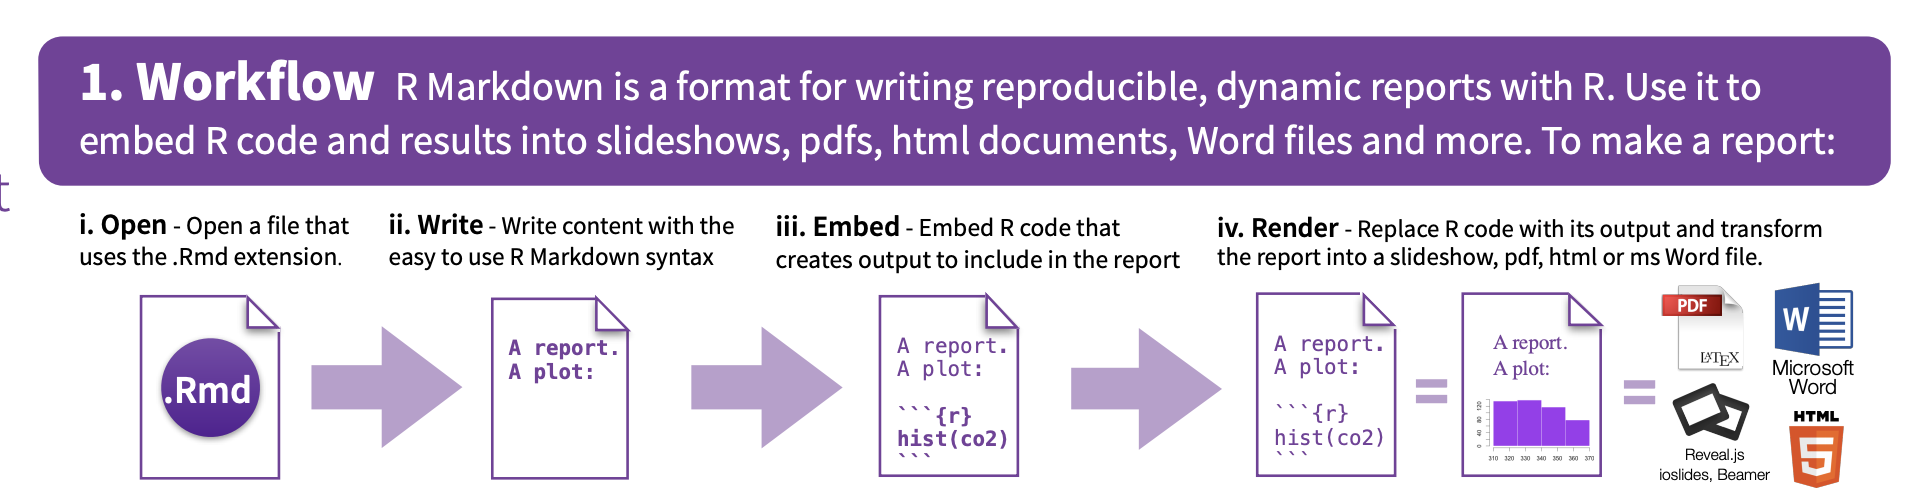
\includegraphics{images/workflow.png}
\caption{}
\end{figure}

\section{Opening a New File}\label{opening-a-new-file}

Writing R Markdown files is easiest within R Studio. Navigate to File
\textgreater{} New File \textgreater{} R Markdown to create a new file.

\begin{figure}
\centering
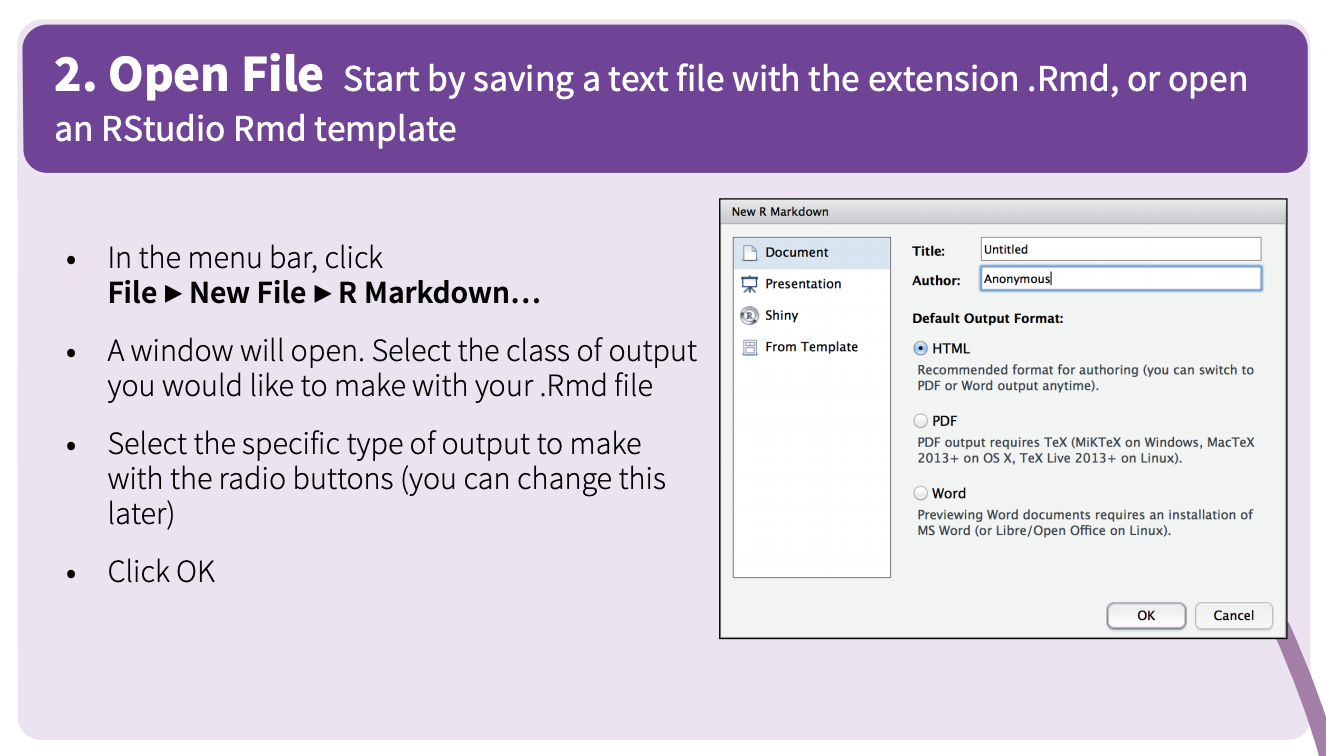
\includegraphics{images/open.png}
\caption{}
\end{figure}

\section{Helpful Syntax}\label{helpful-syntax}

Take a look through helpful sytax in this photo:

\begin{figure}
\centering
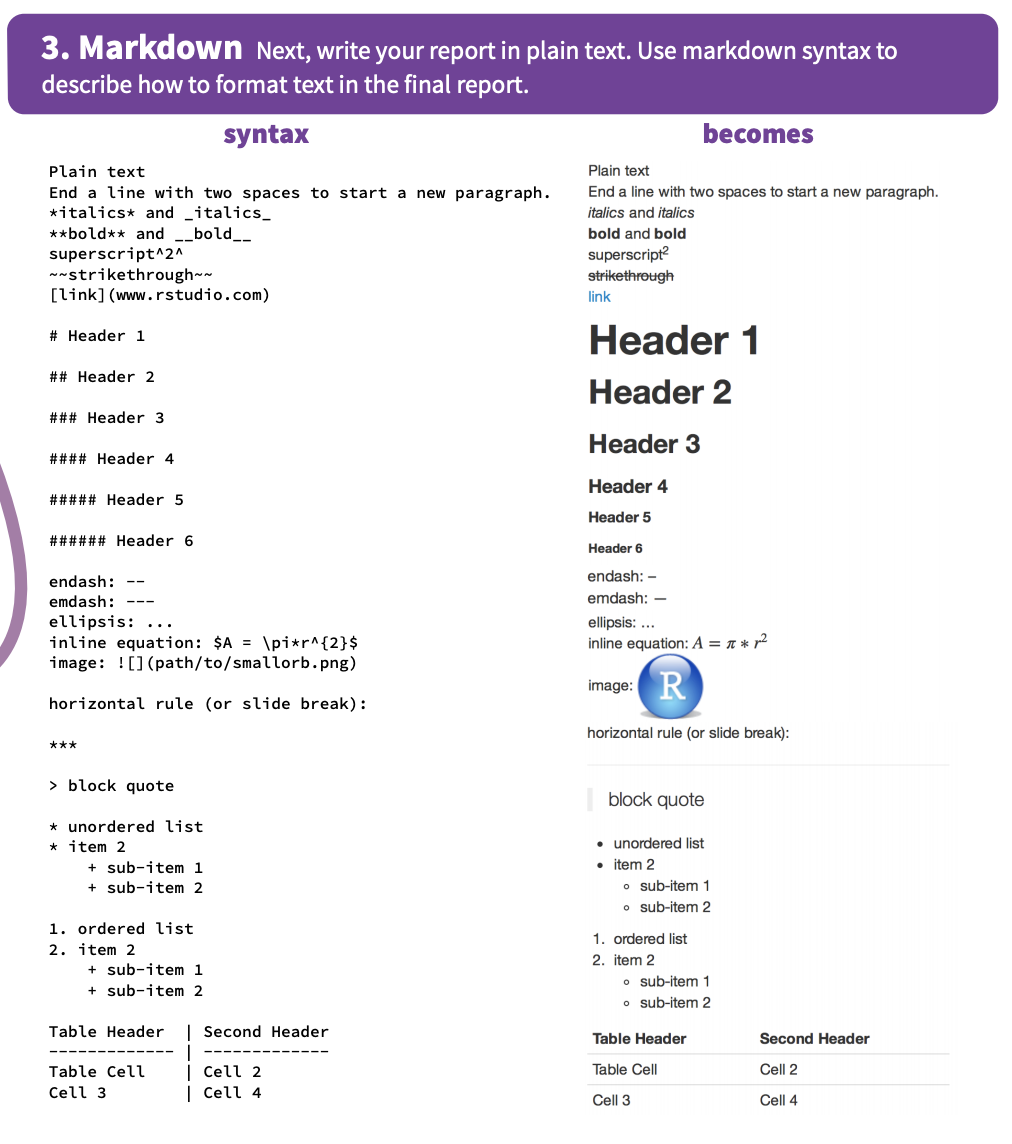
\includegraphics{images/syntax.png}
\caption{}
\end{figure}

Here are some examples to vie. Take a look at the raw R Markdown to view
the syntax in pratice.

\emph{italics} \textbf{bold} \sout{strikethrough}

\begin{quote}
Block Quote
\end{quote}

\begin{itemize}
\tightlist
\item
  Bullets
\item
  Bullets
\item
  subitem
\end{itemize}

\begin{enumerate}
\def\labelenumi{\arabic{enumi}.}
\tightlist
\item
  Lists
\item
  Lists
\end{enumerate}

\begin{itemize}
\tightlist
\item
  subitem
\end{itemize}

\section{Embed Code}\label{embed-code}

One of the best features of R Markdown is the ability to add code to
your document. To add a code snippet, click on the green \emph{insert}
button in your R Studio tool bar and choose which language you would
like to use!

\begin{Shaded}
\begin{Highlighting}[]
\KeywordTok{print}\NormalTok{(}\StringTok{"This is an R code snippet"}\NormalTok{)}
\end{Highlighting}
\end{Shaded}

\begin{verbatim}
## [1] "This is an R code snippet"
\end{verbatim}

\begin{Shaded}
\begin{Highlighting}[]
\BuiltInTok{print}\NormalTok{(}\StringTok{"This is a python code snippet with eval=FALSE"}\NormalTok{)}
\end{Highlighting}
\end{Shaded}

\begin{Shaded}
\begin{Highlighting}[]
\BuiltInTok{echo}\NormalTok{ this a bash code snippet}
\end{Highlighting}
\end{Shaded}

\begin{verbatim}
## this a bash code snippet
\end{verbatim}

\begin{figure}
\centering
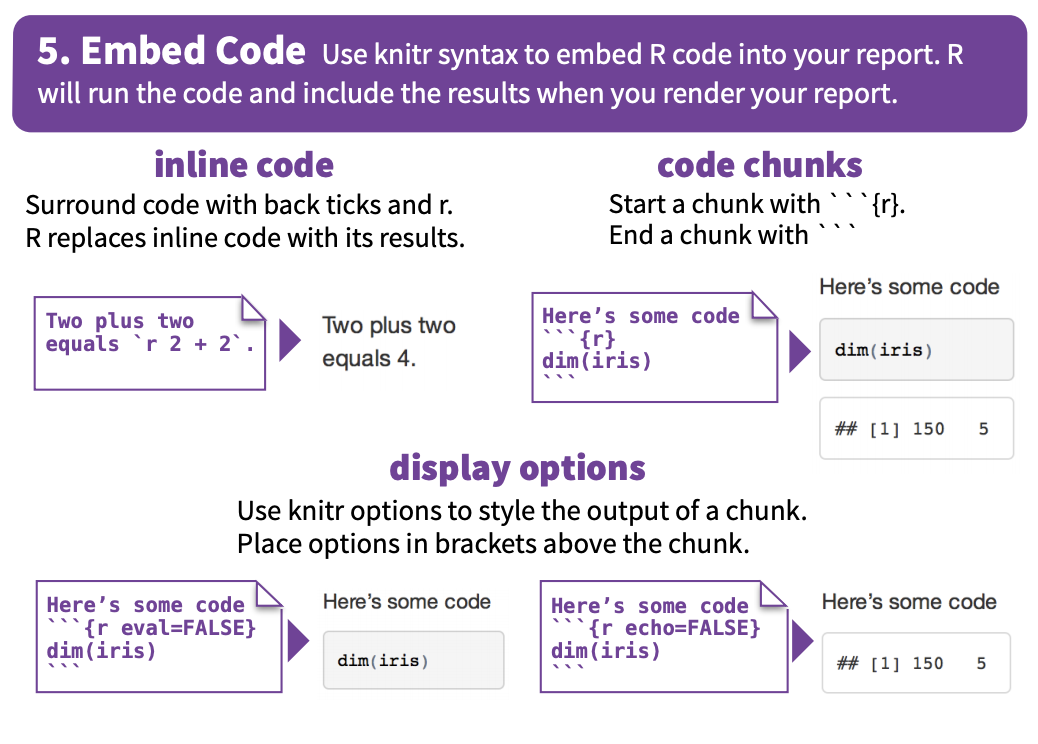
\includegraphics{images/code.png}
\caption{}
\end{figure}

There are also many options for your code snippets. Take a look:

\begin{figure}
\centering
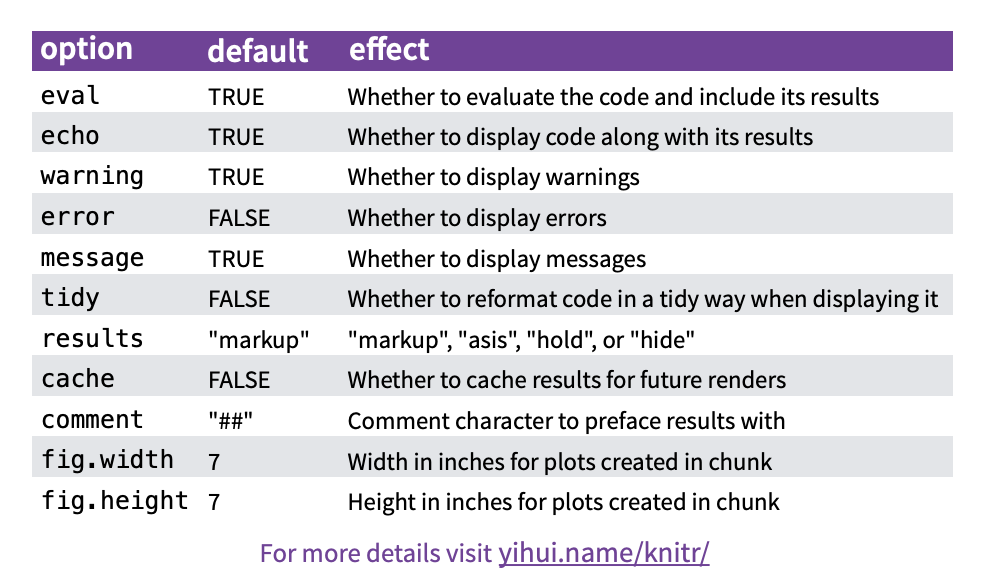
\includegraphics{images/options.png}
\caption{}
\end{figure}

\section{Wrapping (or knitting) it Up}\label{wrapping-or-knitting-it-up}

To knit your Markdown file you click the blue \emph{knit} button in your
R Studio toolbar. You can choose which file format you would like to
knit to as well!

For the purposes of our Merck-Data Mine documentation book, however, we
will not have to knit anything because we are placing the individual
documents in one bookdown book. To learn more about bookdown take a look
at \url{https://bookdown.org/yihui/bookdown/introduction.html} for more
information.

\chapter{Documentation Template}\label{documentation-template}

\section{Introduction}\label{introduction-1}

This section will give an overview of what was accomplished during the
previous sprint.

\section{Code}\label{code}

This section is where important code can be documented and commented on.
Some teams do not need to include all their code here as this would get
excessive. However, important functions or classes should be documented
and discussed here.

\section{Flow Diagrams /
Visualizations}\label{flow-diagrams-visualizations}

This is where teams should showcase flow diagrams of functions, data
pipeline, etc. This might also be a good place for
visualization/screenshots.

\section{White Paper}\label{white-paper}

When important decision are made, such as software specifications or
product developments, they should be documented in this section. Teams
should explain how they came to the conclusion and key takeaways about
the decision.

\section{Technical Report}\label{technical-report}

This section is where teams can highlight the processes of their work.
This is a more in depth look into what was accomplised during the sprint
where teams should describe step by step development.

\chapter{Data Engineering Fall 2020
Documentation}\label{data-engineering-fall-2020-documentation}

\section{Introduction to the Team}\label{introduction-to-the-team}

Our data engineering team is comprised of 6 team members all with unique
skills and backgrounds. The team worked hard to utilize each member's
strengths to help accomplish the semester goals for this project.

Include a brief sentence including your name, major, year, and relevant
experience to the data mine.

Jennifer Leising: I am a 3rd year graduate student in Industrial
Engineering. My research is focused on healthcare and data analytics,
and I have experience working in Clinical trials for a large Pharma
company. Eric Yap: I am sophomore majoring in data science and finance.
Most of my classes have helped developed my Python and R skills, which
are very transferable to the work I do in the data mine. Allison Hill: I
am a senior majoring in electrical engineering. I have coding experience
in various languages, including some Python and R which were used within
this project. Joshua Kosnoff: I am a junior majoring in biomedical
engineering. I perform research with the cancer research center, where I
have previously learned Python for data management and basic analysis.
Karthik Ravishankar: I am a freshman majoring in data science. I have
learned Java in highschool and at Purdue and some Python which was self
taught to contribute to the project. Pranav Anandarao: I am a sophomore
majoring in computer engineering. I have experience in a few different
programming languages, including Python. I also have previous experience
working on clinical applications.

\section{Semester Goals}\label{semester-goals}

The overall aim of this project was to create a method to collect
continuous data from patients in clinical trials. The biometrics team
decided to do this by collecting data from Fitbit devices and developing
an application to collect supplementary data from the users.

The data engineering team's task was to collect the data and put it into
a usable format for storage with the data architecture team. This
semester, our goal was to add functionality to collect data from
multiple users and handle data coming in from different devices.
Furthermore, we would like to be able to schedule the program to collect
the user data periodically.

\section{Data Overview}\label{data-overview}

\subsection{Fitbit Devices vs.~Apple
Watch}\label{fitbit-devices-vs.apple-watch}

The 2019-2020 Merck Biometric team used the Fitbit to gather data for
the project. The Merck stakeholder's had also mentioend wanting to
explore the Apple Watch to reach additional populations. Our team wanted
to better understand what data was available from each company's
devices. As a note, we listed all the features that would be available
from any device. We created the chart below to list the features
available on each device. We found very similar data to be available on
both devices.

\begin{verbatim}
            |                                       |Fitbit         |Apple Watch
\end{verbatim}

---------------\textbar{}---------------------------------------\textbar{}---------------\textbar{}---------------
Activity \textbar{}Steps \textbar{}X \textbar{}X \textbar{}Workouts
\textbar{}X \textbar{}X \textbar{}Sit/Stand \textbar{}X* \textbar{}NA
\textbar{}Flight Climbed \textbar{}X \textbar{}X \textbar{}Elevation
\textbar{}X \textbar{}X \textbar{}Time spent in different activity
levels\textbar{}X \textbar{}X \textbar{}Calories burned \textbar{}X
\textbar{}X Sleep \textbar{}Asleep vs Awake \textbar{}X \textbar{}X
\textbar{}Stages \textbar{}X \textbar{}NA Heart Rate \textbar{}Time
spent in different heart ranges \textbar{}X \textbar{}3rd party apps
\textbar{}Resting heart rate \textbar{}X \textbar{}X \textbar{}Walking
Heartrate \textbar{}NA \textbar{}X \textbar{}Heart rate during activity
\textbar{}X \textbar{}X \textbar{}Intraday Tracking \textbar{}5 sec
\textbar{}10 min Nutrition \textbar{}Food log* \textbar{}X \textbar{}X
\textbar{}Water log* \textbar{}X \textbar{}X Body/Weight \textbar{}BMI*
\textbar{}X \textbar{}X \textbar{}Weight* \textbar{}X \textbar{}X
Additional \textbar{}ECG \textbar{}Coming soon \textbar{}X
\textbar{}Blood Oxygen \textbar{}X \textbar{}X \textbar{}Fall Detection
\textbar{}X \textbar{}X \textbar{}Skin Thermometer \textbar{}X
\textbar{}NA \textbar{}Ear Health \textbar{}NA \textbar{}X
\textbar{}Stress Response \textbar{}X \textbar{}NA
---------------------------------------------------------------------------------------
*Entered manually NA = Not Available

With the Apple Watch, most data tracking is through the Health app and
the files are exported as a .xml, which is difficult to read. However,
you can also export your data through the Health app and have it opened
in Numbers/Excel for easy viewing. For the FitBit, activity is recorded
through the watch and outputs a .csv file when exporting, which is easy
to read and open in applications like Excel and Numbers.

Additionally, it appears we are able to use Python in order to
gather/sort data on both the Apple watch and Fitbit devices. Data is
able to be read through pandas. Since Apple Watch returns a .xml file,
we have to parse it first and use xmltodict module within Python before
we can start applying functions to our data.

Based on the scope for this semester, we did not do further research
into the Apple Watch data collection, but this is one of our goal's for
the coming Spring semester.

\subsection{Data Collected from Fitbit
Devices}\label{data-collected-from-fitbit-devices}

Our team collected data that can be grouped into several major
categories:

\begin{verbatim}
Device: Device Name

Activites: totalDistance, veryActiveDistance, moderatleyActiveDistance, lightlyActiveDistance, veryActiveMinutes, fairlyActiveMinutes, 
lightlyActiveMinutes, sedentaryMinutes, floorsClimbed, daySteps, intraday data

Sleep: sleepEfficiency, minutesAsleep

Heart Rate: HRrange30to100, HRrange100to140, HRrange140to170, HRrange170to220, avgRestingHR, intraday data

Weight: weight, BMI
\end{verbatim}

\section{Scaling the Framework}\label{scaling-the-framework}

The framework for collecting biometric data from Fitbit's API was
previously established and can be found in the
\href{https://nicholasrosenorn.github.io/wearables-book/tutorial-data-capture-in-python.html\#authentication}{Merck
Wearables Book section 8}. However, this framework could only be used to
collect one user's data at a time, and needed to be manually monitored
to switch between browser and python windows. Further, the framework
assumed that the user's Fitbit device would be the Fitbit Ionic. In
order to make this project upscalable, the framework needed to be
modified to support multiple users in an automizable way and to account
for multiple device types.

\subsection{Multiple Users}\label{multiple-users}

\subsubsection{Supporting Multiple Users Via Accessing
Credentials}\label{supporting-multiple-users-via-accessing-credentials}

To support multiple users, a database of multiple user login credentials
needed to be created. There is an ongoing collaboration with the Front
End team to create a more secure storage system, but for now credentials
are stored in a csv file with the format ``username,password''. With the
usernames and passwords stored in this way, a login array can be created
that will be used to plug into the automated process.

\begin{Shaded}
\begin{Highlighting}[]
\CommentTok{# Initialize Emails and Passwords lists}
\NormalTok{Emails }\OperatorTok{=}\NormalTok{ []}
\NormalTok{Passwords }\OperatorTok{=}\NormalTok{ []}
\CommentTok{# Create Emails and Passwords lists from Fitbit_Credentials.csv}
\ControlFlowTok{with} \BuiltInTok{open}\NormalTok{(}\StringTok{"Fitbit_Credentials.csv"}\NormalTok{) }\ImportTok{as}\NormalTok{ File1:}
\NormalTok{    IDs }\OperatorTok{=}\NormalTok{ csv.DictReader(File1)}
    \ControlFlowTok{for}\NormalTok{ row }\KeywordTok{in}\NormalTok{ IDs:}
\NormalTok{        Emails.append(row[}\StringTok{'Username'}\NormalTok{])}
\NormalTok{        Passwords.append(row[}\StringTok{'Password'}\NormalTok{])}
\end{Highlighting}
\end{Shaded}

As previously mentioned, the previous framework was not set up for
running through multiple accounts. To solve this issue, it was
reformatted into iterative-friendly components. The first of which is
the PythonBot.py file, which both establishes the login arrays outlined
above and is responsible for coordinating the other file and function
calls to make this process run smoothly.

\begin{Shaded}
\begin{Highlighting}[]
\CommentTok{# import other codes}
\ImportTok{import}\NormalTok{ BiometricPrevious}
\ImportTok{import}\NormalTok{ gather_keys_oauth2 }\ImportTok{as}\NormalTok{ Oauth2}
\KeywordTok{class}\NormalTok{ FitbitBot:}
    \KeywordTok{def} \FunctionTok{__init__}\NormalTok{(}\VariableTok{self}\NormalTok{, EMAIL, PASSWORD, DATE):}
        \CommentTok{#Both the Client ID and Client Secret come from when Fitbit site after registering an app}
\NormalTok{        CLIENT_ID }\OperatorTok{=} \StringTok{'22BH28'} 
\NormalTok{        CLIENT_SECRET }\OperatorTok{=} \StringTok{'78a4838804c1ff0983591e69196b1c46'}
        
        \CommentTok{#Authorization Process}
\NormalTok{        server }\OperatorTok{=}\NormalTok{ Oauth2.OAuth2Server(CLIENT_ID, CLIENT_SECRET)}
\NormalTok{        server.browser_authorize(EMAIL, PASSWORD)}
\NormalTok{        ACCESS_TOKEN }\OperatorTok{=} \BuiltInTok{str}\NormalTok{(server.fitbit.client.session.token[}\StringTok{'access_token'}\NormalTok{])}
\NormalTok{        REFRESH_TOKEN }\OperatorTok{=} \BuiltInTok{str}\NormalTok{(server.fitbit.client.session.token[}\StringTok{'refresh_token'}\NormalTok{])}
\NormalTok{        auth2_client }\OperatorTok{=}\NormalTok{ fitbit.Fitbit(CLIENT_ID, CLIENT_SECRET, Oauth2}\OperatorTok{=}\VariableTok{True}\NormalTok{, access_token}\OperatorTok{=}\NormalTok{ACCESS_TOKEN,}
\NormalTok{        refresh_token}\OperatorTok{=}\NormalTok{REFRESH_TOKEN)}
\NormalTok{        BiometricPrev }\OperatorTok{=}\NormalTok{ BiometricPrevious.FitbitModel1(auth2_client)}
        
\NormalTok{        biometricDF }\OperatorTok{=}\NormalTok{ BiometricPrev.getBiometricData(DATE) }\CommentTok{#append to data frame}
\NormalTok{        biometricDF.to_csv(}\StringTok{'./user'} \OperatorTok{+} \BuiltInTok{str}\NormalTok{(i) }\OperatorTok{+} \StringTok{'_'} \OperatorTok{+}\NormalTok{ DATE }\OperatorTok{+} \StringTok{'.csv'}\NormalTok{)}
        \BuiltInTok{print}\NormalTok{(}\StringTok{"Python Script Executed"}\NormalTok{)}
\CommentTok{# Run data extraction}
\ControlFlowTok{for}\NormalTok{ i }\KeywordTok{in} \BuiltInTok{range}\NormalTok{(}\BuiltInTok{len}\NormalTok{(Emails)):}
    \ControlFlowTok{for}\NormalTok{ j }\KeywordTok{in} \BuiltInTok{range}\NormalTok{(}\DecValTok{1}\NormalTok{): }\CommentTok{# Call the previous 1 days worth of info <-- will be replaced with cronjob}
\NormalTok{        today }\OperatorTok{=} \BuiltInTok{str}\NormalTok{((datetime.datetime.now() }\OperatorTok{-}\NormalTok{ datetime.timedelta(j)).strftime(}\StringTok{"%Y-%m-}\SpecialCharTok{%d}\StringTok{"}\NormalTok{))}
\NormalTok{        FitbitBot(Emails[i], Passwords[i], today)}
\end{Highlighting}
\end{Shaded}

The \emph{BiometricPrevious} file contains the remainder of the previous
framework with data collection functions, but it was also altered to
allow for multiple devices. More information about his can be found in
the \textbf{Multiple Devices} section of this report. The line
\emph{biometric.to\_csv} will store the collected data in a csv format
with a title of *user\#\_DATE\emph{, where }user\#* corresponds to the
order at which the user's login credentials are stored in the
credentials csv database.

\subsubsection{Supporting Multiple Users Via Allowing for
Automation}\label{supporting-multiple-users-via-allowing-for-automation}

In order to create an automation bot to regularly call the data
collection code (see \textbf{Scheduling Our Data Collection} for more
information on this), the code had to be adjusted so that it did not
open browser windows, as the opening of browser windows was found to
stall the bot. In order to accomplish this, the Selenium module was
used. Official Selenium documentation can be found
\href{https://selenium-python.readthedocs.io}{here}.

Since Selenium was not already downloaded on the device, it needed to be
installed. To do this, the following was typed into a Terminal window:

\begin{Shaded}
\begin{Highlighting}[]
\NormalTok{pip install selenium}
\end{Highlighting}
\end{Shaded}

To use Selenium in a code, the libraries and packages will need to be
imported. Since \emph{gather\_keys\_oauth2.py} is the only code package
responsible for accessing websites, Selenium only needs to be imported
into that document. To do this, the following code was added to
\emph{gather\_keys\_oauth2.py}.

\begin{Shaded}
\begin{Highlighting}[]
\ImportTok{from}\NormalTok{ selenium }\ImportTok{import}\NormalTok{ webdriver}
\ImportTok{from}\NormalTok{ selenium.webdriver }\ImportTok{import}\NormalTok{ Firefox}
\ImportTok{from}\NormalTok{ selenium.webdriver.firefox.options }\ImportTok{import}\NormalTok{ Options}
\ImportTok{from}\NormalTok{ selenium.webdriver.common.by }\ImportTok{import}\NormalTok{ By}
\end{Highlighting}
\end{Shaded}

Strictly speaking, the only explicitly needed code would be \emph{import
Selenium}. However, by importing specific functions from the Selenium
library upfront, notation later on was simplified. This can be seen
below when firefox options were set. Instead of calling
\emph{Selenium.webdriver.firefox.options} every line, \emph{Options} was
able to be called instead.

The appropriate Selenium firefox browser driver was downloaded
\href{https://github.com/mozilla/geckodriver/releases}{here}.

\textbf{Note} it does not matter where the driver is installed, but its
installation path needs to be plugged into the gather\_keys\_oath2.py
code. For those following along with the guide, make a note of the
installation path.

The following block of code was written to set the Selenium webdriver
functions.

\begin{Shaded}
\begin{Highlighting}[]
\NormalTok{firefox_options }\OperatorTok{=}\NormalTok{ Options()}
\NormalTok{firefox_options.add_argument(}\StringTok{"window-size=1920,1080"}\NormalTok{)}
\NormalTok{firefox_options.add_argument(}\StringTok{"--headless"}\NormalTok{)}
\NormalTok{firefox_options.add_argument(}\StringTok{"start-maximized"}\NormalTok{)}
\NormalTok{firefox_options.add_argument(}\StringTok{"--disable-infobars"}\NormalTok{)}
\NormalTok{firefox_options.add_argument(}\StringTok{"--disable-extensions"}\NormalTok{)}
\NormalTok{firefox_options.add_argument(}\StringTok{"--no-sandbox"}\NormalTok{)}
\NormalTok{firefox_options.add_argument(}\StringTok{"--disable-dev-shm-usage"}\NormalTok{)}
\NormalTok{firefox_options.binary_location }\OperatorTok{=} \StringTok{'/class/datamine/apps/firefox/firefox'}
\end{Highlighting}
\end{Shaded}

Adjust the path in the final option,
\emph{firefox\_options.binary\_location}, accordingly. The other main
option of interest is
\emph{firefox\_options.add\_argument(``--headless'')}. This
\emph{headerless} option is what allows the code to access the Fitbit
website without actually opening a browser -- effectively, Python
becomes a browser simulator. This is the main reason Selenium was used.
The other options are for optimal performance, but not strictly
necessary.

The first time an account is added, manual permissions will need to be
granted to Fitbit's authorization website. To do this, comment out this
headerless option (place a ``\#'' before the line), run the
\emph{PythonBot.py} code, and check the permissions boxes for each new
account as it pops up. After doing this once, uncomment this headerless
line. The system will then be ready for full automation.

The official Selenium documentation also supports a Google Chrome
driver. If Chrome is preferred, it can be substituted in for FireFox
without issue. However, make sure to change all instances of
\emph{firefox} in the above codes to \emph{Chrome.}

With Selenium downloaded and imported, the last step was to call and use
Selenium. The following line in \emph{browser\_authorize} function in
\emph{gather\_keys\_oauth2.py} was responsible for opening the web
browser, so it was targeted for edits.

\begin{Shaded}
\begin{Highlighting}[]
\NormalTok{    threading.Timer(}\DecValTok{1}\NormalTok{, webbrowser.}\BuiltInTok{open}\NormalTok{, args}\OperatorTok{=}\NormalTok{(url,)).start()}
\end{Highlighting}
\end{Shaded}

As its name might suggest, the \emph{webbrowser.open} function causes a
web browser to open. The other passed arguments \emph{1} and
\emph{args=(url,)} are parameters that can be left unchanged. This line
was replaced with the following code:

\begin{Shaded}
\begin{Highlighting}[]
\NormalTok{    driver }\OperatorTok{=}\NormalTok{ webdriver.Firefox(executable_path }\OperatorTok{=} \StringTok{'/class/datamine/apps/geckodriver'}\NormalTok{, options}\OperatorTok{=}\NormalTok{firefox_options)}
\NormalTok{    driver.get(}\StringTok{"https://accounts.fitbit.com/login?targetUrl=https%3A}\SpecialCharTok{%2F%2F}\StringTok{www.fitbit.com}\SpecialCharTok{%2F}\StringTok{us}\SpecialCharTok{%2F}\StringTok{home"}\NormalTok{)}
\NormalTok{    sleep(}\DecValTok{5}\NormalTok{)}
\NormalTok{    driver.find_element(By.XPATH, }\StringTok{"//input[@type='email']"}\NormalTok{).send_keys(email)}
\NormalTok{    sleep(}\DecValTok{2}\NormalTok{)}
\NormalTok{    driver.find_element(By.XPATH, }\StringTok{"//input[@type='password']"}\NormalTok{).send_keys(password)}
\NormalTok{    sleep(}\DecValTok{2}\NormalTok{)}
\NormalTok{    driver.find_element(By.XPATH, }\StringTok{"/html/body/div[2]/div/div[2]/div/div/div[3]/form/div[4]/div/button"}\NormalTok{).click()}
\NormalTok{    sleep(}\DecValTok{10}\NormalTok{)}
    
\NormalTok{    threading.Timer(}\DecValTok{1}\NormalTok{, driver.get, args}\OperatorTok{=}\NormalTok{(url,)).start()}
\end{Highlighting}
\end{Shaded}

The first line of the following code initializes the Selenium webdriver.
Edit the \emph{executable\_path} as needed based on where the firefox
driver was installed. The next line, \emph{driver.get}, tells the
Selenium web browser what website to go to. The \emph{find\_elements}
commands are what allow for the automatization of plugging in usernames
and emails. The sleep functions are input time delays to help make sure
that the website has time to properly load before attempting to log in.
The final line should look familiar. It is the same as the original
line, except replacing the \emph{webbrowser.open}, which opens a normal
web browser, with \emph{driver.get}, which calls Selenium's browser
simulator. The rest of \emph{gather\_keys\_oauth2} can remain as is.

\subsubsection{Moving to Scholar}\label{moving-to-scholar}

When multiple user logins were pushed and data extractions were
performed in relatively quick succession on personal Wi-Fi, Fitbit's
cybersecurity software flagged and temporarily banned the IP address
from accessing their site. While these bans can be overturned by
contacting Fitbit's customer support page on Twitter, the ``unbanning''
is temporary. This leads to a cycle of getting banned and asking to be
unbanned, which is both inconvenient and detrimental to any long term
data collection plans. The hope with Scholar is that, as an educational
IP address, it can be whitelisted and the automated process can function
without getting users banned.

\paragraph{Using Scholar}\label{using-scholar}

To access Scholar, go to
*\url{https://scholar-fe03.rcac.purdue.edu:300/main/*} and login with
Purdue 2 Factor Credentials.

The codes used for this part of the project are written in Python.
Unfortunately, Scholar does not currently support Python IDEs (Spyder,
VS code, etc). This means that the code either needs to be called
through a Jupyter Notebook Kernel or through a terminal window. For now,
the code will be run via Terminal commands.

To open Terminal, click on \textbf{Terminal Emulator} in Scholar's
applications bar. Once Terminal is open, navigate to the \emph{/class}
directory and then to the appropriate folder. To do this, type the
following commands into Terminal:

\begin{Shaded}
\begin{Highlighting}[]
\NormalTok{cd ..}
\NormalTok{cd ..}
\NormalTok{cd }\OperatorTok{/}\KeywordTok{class}\OperatorTok{/}\NormalTok{datamine}\OperatorTok{/}\NormalTok{corporate}\OperatorTok{/}\NormalTok{merck}\OperatorTok{/}\NormalTok{DataEngineers}\OperatorTok{/}\NormalTok{Fitbit}
\end{Highlighting}
\end{Shaded}

Needed files and libraries have been installed on Scholar. Pathways
within the code have been adjusted to Scholar's directory. As a result,
there is only one more step that needs to be done before the code can be
run. This step is to direct the python3 program where to find installed
libraries. Type the following command into the Terminal:

\begin{Shaded}
\begin{Highlighting}[]
\NormalTok{source }\OperatorTok{/}\KeywordTok{class}\OperatorTok{/}\NormalTok{datamine}\OperatorTok{/}\NormalTok{apps}\OperatorTok{/}\NormalTok{python.sh}
\end{Highlighting}
\end{Shaded}

\textbf{Note} You will need to rerun this command everytime you close
out of Terminal and reopen it.

Now, Scholar is ready to run PythonBot.py! To run the code, type the
following into Terminal:

\begin{Shaded}
\begin{Highlighting}[]
\NormalTok{python3 PythonBot.py}
\end{Highlighting}
\end{Shaded}

\textbf{Note} if the previous Terminal window was closed, navigate to
\emph{/class/datamine/corporate/merck/DataEngineers/Fitbit} again before
running \emph{python3 PythonBot.py}

Extracted data is formatted into CSV files and accessible at
\emph{/class/datamine/corporate/merck/DataEngineers/Fitbit/CSV\_Files}.

\subsection{Multiple Devices}\label{multiple-devices}

Not all fitbit devices have the same data available to them. This is
most noticeable in older models, in which functionality such as the
number of floors climbed or sleep cycles was not yet implemented. Using
the get\_Devices function available in the Fitbit API, the code returns
a string corresponding to the Fitbit version. For example, a Fitbit
Ionic would return the string ``Ionic''. Using this information, if-else
statements were implemented to check the version and assign
corresponding data values. Data that is not available would be input as
``None'' within the data table. In some cases, the function can simply
check if the data is NULL and automatically do this such as with the
sleep data. However for data such as activity levels, the data gets
input as a ``0'' instead and thus needs a check. Checks for some of the
newer models have been implemented, along with a generic case. The table
below shows the implemented models and their available data: \textbar{}
\textbar{}Ionic \textbar{} Versa Lite \textbar{}Inspire \textbar{}Charge
3 \textbar{}
---------------\textbar{}---------------------------------------\textbar{}--------------\textbar{}-------------\textbar{}-------------\textbar{}-------------\textbar{}
Activity \textbar{}Steps \textbar{}X \textbar{}X \textbar{}X \textbar{}X
\textbar{} \textbar{}Workouts \textbar{}X \textbar{}X \textbar{}
\textbar{} \textbar{} \textbar{}Sit/Stand \textbar{}X \textbar{}X
\textbar{} \textbar{} \textbar{} \textbar{}Flight Climbed \textbar{}X
\textbar{} \textbar{} \textbar{} \textbar{} \textbar{}Elevation
\textbar{}X \textbar{} \textbar{} \textbar{} \textbar{} \textbar{}Time
spent in different activity levels\textbar{}X \textbar{}X \textbar{}
\textbar{} \textbar{} \textbar{}Calories burned \textbar{}X \textbar{}X
\textbar{} \textbar{} \textbar{} Sleep \textbar{}Asleep vs Awake
\textbar{}X \textbar{}X \textbar{}X \textbar{}X \textbar{}
\textbar{}Stages \textbar{}X \textbar{}X \textbar{} \textbar{}
\textbar{} Heart Rate \textbar{}Time spent in different heart ranges
\textbar{}X \textbar{}X \textbar{} \textbar{}X \textbar{}
\textbar{}Resting heart rate \textbar{}X \textbar{}X \textbar{}
\textbar{}X \textbar{} \textbar{}Walking Heartrate \textbar{}X
\textbar{}X \textbar{} \textbar{}X \textbar{} \textbar{}Heart rate
during activity \textbar{}X \textbar{}X \textbar{} \textbar{}X
\textbar{}
-----------------------------------------------------------------------------------------------------------------

The following function is what is used to obtain the device model
string:

\begin{Shaded}
\begin{Highlighting}[]
\KeywordTok{def}\NormalTok{ getDevice():}
\NormalTok{    devices }\OperatorTok{=}\NormalTok{ auth2_client.get_devices()}
    \ControlFlowTok{if}\NormalTok{(}\BuiltInTok{len}\NormalTok{(devices) }\OperatorTok{==} \DecValTok{0}\NormalTok{):}
\NormalTok{        deviceVersion }\OperatorTok{=} \StringTok{'None'}
    \ControlFlowTok{else}\NormalTok{:}
\NormalTok{        deviceVersion }\OperatorTok{=}\NormalTok{ devices[}\DecValTok{0}\NormalTok{][}\StringTok{'deviceVersion'}\NormalTok{]    }
    \ControlFlowTok{return}\NormalTok{ deviceVersion}
\end{Highlighting}
\end{Shaded}

The function first calls the built-in Fitbit API get\_devices(). Next it
checks the length of the output to determine if it is valid. If it is
not valid, the user must not have any device registered. At the moment,
the code only obtains the first device if a user has multiple
registered.

\section{Scheduling the Data
Collection}\label{scheduling-the-data-collection}

Through using the CronTab module within Python, we are able to schedule
and run our FitBit functions on a routinely basis. The data we collect
is stored in a dataframe and new data is continuously appended to this
dataframe. The scheduled time is set to every 9 AM on weekdays.

\section{Collaborating with other
Teams}\label{collaborating-with-other-teams}

Our team had three main interactions with the other teams. The first one
was with the Data Architects. When reviewing last year's code, we
noticed that sending a CSV file everytime would be inneficient. We
discovered a function, dataFrame.to\_sql(), which would allow the data
to be sent straight into the SQL server. Although a solution was found,
we decided to leave the code how it is and save this idea for another
day. The second and third interactions were with the Front End team. The
first time, we wanted to see if there was a way to easily collect the
user's fitbit username and password. The Front End team was able to
create a way to have the login information collected from mobile app and
saved on the SQL server with the help of the Back End team. This was a
very important problem to solve as the API needs to log into the user's
fitbit account to pull their data. Our last collaboration was regarding
a issue that would result in complications during the clinical trial.
Regardless of whether the user is wearing their device or not, any time
the fitbit wasn't in an active motion, time is accrued on the user's
sedentary minutes. This would be a problem as there is no way to
differentiate whether the user was sedentary, or if the fitbit wasn't on
the user. After conversing with the Front End team, we decided that an
alert system or question during their survey would help solve this
issue. This problem is a work in progress and doesn't have a solution as
of yet.

\section{Future Work}\label{future-work}

Our future work for the Spring 2021 semester seeks to build upon our
work completed during this Fall 2020 semester. Our main goals are listed
include: (1) streamlining our work with the other Merck biometric teams
to ensure the entire process works well from start to finish, (2)
exploring alternative ways to access the user's fitbit information that
might better align with the way fitbit intends multiple user data
collection, and (3) investigating the collection of data from the Apple
Watch.

\begin{enumerate}
\def\labelenumi{(\arabic{enumi})}
\tightlist
\item
  Streamlining work with the other Merck Biometric teams
\item
  Exploring alternative ways to access the user's fitbit information
\item
  Investigating the collection of data from the Apple Watch
\end{enumerate}

\chapter{Data Engineering Spring 2021
Documentation}\label{data-engineering-spring-2021-documentation}

\section{Completing the Pipeline}\label{completing-the-pipeline}

In order to connect data collection process to the rest of the pipeline,
it had to be able to read patient information and login credentials from
the SQL database, as well as automatically append the collected
biometric data to a database. In order to accomplish this, the
PythonBot.py code had to be able to connect to SQL. This was done by
first importing the necessary sqlachemy pacakges and then establishing a
connection to our specific database.

To import packages:

\begin{Shaded}
\begin{Highlighting}[]
\CommentTok{# using sqlalchemy}
\ImportTok{import}\NormalTok{ sqlalchemy }\ImportTok{as}\NormalTok{ sal}
\ImportTok{from}\NormalTok{ sqlalchemy }\ImportTok{import}\NormalTok{ create_engine}
\ImportTok{import}\NormalTok{ pandas }\ImportTok{as}\NormalTok{ pd}
\end{Highlighting}
\end{Shaded}

To establish connection to SQL database:

\begin{Shaded}
\begin{Highlighting}[]
\CommentTok{# establish connecttion URL}
\NormalTok{conn }\OperatorTok{=} \StringTok{"mysql+pymysql://}\SpecialCharTok{\{0\}}\StringTok{:}\SpecialCharTok{\{1\}}\StringTok{@}\SpecialCharTok{\{2\}}\StringTok{:}\SpecialCharTok{\{3\}}\StringTok{/}\SpecialCharTok{\{4\}}\StringTok{"}\NormalTok{.}\BuiltInTok{format}\NormalTok{(}
    \StringTok{'cb3i17t0aqn6a4ff'}\NormalTok{, }\StringTok{'e2l4k9zn24shcj42'}\NormalTok{, }\StringTok{'rnr56s6e2uk326pj.cbetxkdyhwsb.us-east-1.rds.amazonaws.com'}\NormalTok{, }\StringTok{'3306'}\NormalTok{, }\StringTok{'lfry112yqr3k2dfr'}\NormalTok{)}
 
\CommentTok{# create engine}
\NormalTok{engine }\OperatorTok{=}\NormalTok{ sal.create_engine(conn)}
\end{Highlighting}
\end{Shaded}

If another SQL database is used in the future, please note that
`cb3i17t0aqn6a4ff' corresponds to `username', `e2l4k9zn24shcj42'
corresponds to `password',
`rnr56s6e2uk326pj.cbetxkdyhwsb.us-east-1.rds.amazonaws.com' corresponds
to `address', `3306' corresponds to `port', and `lfry112yqr3k2dfr'
corresponds to `DB'. Change these values as appropriate in the code.

\subsection{Reading in user data from patient
table}\label{reading-in-user-data-from-patient-table}

Patient data was imported as a series of arrays. The SQL patient table
was read in as df1, which was used to form lists of data corresponding
to individual patient's emails, passwords, IDs, and usernames.

\begin{Shaded}
\begin{Highlighting}[]
\NormalTok{df1 }\OperatorTok{=}\NormalTok{ pd.read_sql_query(}\StringTok{"SELECT * FROM patient"}\NormalTok{, engine)}
\NormalTok{emails }\OperatorTok{=}\NormalTok{ []}
\NormalTok{passwords }\OperatorTok{=}\NormalTok{ []}
\NormalTok{IDs }\OperatorTok{=}\NormalTok{ []}
\NormalTok{usernames }\OperatorTok{=}\NormalTok{ []}
\ControlFlowTok{for}\NormalTok{ i }\KeywordTok{in} \BuiltInTok{range}\NormalTok{(}\BuiltInTok{len}\NormalTok{(df1)):}
\NormalTok{    emails.append(df1.email[i])}
\NormalTok{    passwords.append(df1.fitbit_password[i])}
\NormalTok{    IDs.append(df1.patient_id[i])}
\NormalTok{    usernames.append(df1.username[i])}
\end{Highlighting}
\end{Shaded}

As was previously the case, this data was iterated through and plugged
into the FitbitBot function.

\subsection{Appending user data to SQL
table}\label{appending-user-data-to-sql-table}

Once data was collected (collection functions can be found in
\emph{BiometricPrevious\_getDevice\_v2.py}), it needed to be appended to
the SQL database. A new function was made to reformat the data to have
the same column names as the SQL table.

\begin{Shaded}
\begin{Highlighting}[]
\KeywordTok{def}\NormalTok{ appendDataBase(DATA,ENGINE, USER, ID):}
\NormalTok{    obj }\OperatorTok{=}\NormalTok{ pd.DataFrame()}
   
\NormalTok{    obj[}\StringTok{'patient_id'}\NormalTok{] }\OperatorTok{=}\NormalTok{ [ID]}
\NormalTok{    obj[}\StringTok{'fbusername'}\NormalTok{] }\OperatorTok{=}\NormalTok{ [USER]}
\NormalTok{    obj[}\StringTok{'collection_date'}\NormalTok{] }\OperatorTok{=}\NormalTok{ [DATA.get(}\StringTok{"Date"}\NormalTok{)]}
\NormalTok{    obj[}\StringTok{'steps'}\NormalTok{] }\OperatorTok{=}\NormalTok{ [DATA.get(}\StringTok{"Steps"}\NormalTok{)]}
\NormalTok{    obj[}\StringTok{'floors_climbed'}\NormalTok{] }\OperatorTok{=}\NormalTok{ [DATA.get(}\StringTok{"Floors Climbed"}\NormalTok{)]}
\NormalTok{    obj[}\StringTok{'total_miles'}\NormalTok{] }\OperatorTok{=}\NormalTok{ [DATA.get(}\StringTok{"Total Miles"}\NormalTok{)]}
\NormalTok{    obj[}\StringTok{'lightly_active_miles'}\NormalTok{] }\OperatorTok{=}\NormalTok{ [DATA.get(}\StringTok{"Lightly Active Miles"}\NormalTok{)]}
\NormalTok{    obj[}\StringTok{'moderately_active_miles'}\NormalTok{] }\OperatorTok{=}\NormalTok{ [DATA.get(}\StringTok{"Moderately Active Miles"}\NormalTok{)]}
\NormalTok{    obj[}\StringTok{'very_active_miles'}\NormalTok{] }\OperatorTok{=}\NormalTok{ [DATA.get(}\StringTok{"Very Active Miles"}\NormalTok{)]}
\NormalTok{    obj[}\StringTok{'sedentary_minutes'}\NormalTok{] }\OperatorTok{=}\NormalTok{ [DATA.get(}\StringTok{"Sedentary Minutes"}\NormalTok{)]}
\NormalTok{    obj[}\StringTok{'lightly_active_minutes'}\NormalTok{] }\OperatorTok{=}\NormalTok{ [DATA.get(}\StringTok{"Lightly Active Minutes"}\NormalTok{)]}
\NormalTok{    obj[}\StringTok{'fairly_active_minutes'}\NormalTok{] }\OperatorTok{=}\NormalTok{ [DATA.get(}\StringTok{"Fairly Active Minutes"}\NormalTok{)]}
\NormalTok{    obj[}\StringTok{'very_active_minutes'}\NormalTok{] }\OperatorTok{=}\NormalTok{ [DATA.get(}\StringTok{"Very Active Minutes"}\NormalTok{)]}
\NormalTok{    obj[}\StringTok{'hr30_100_minutes'}\NormalTok{] }\OperatorTok{=}\NormalTok{ [DATA.get(}\StringTok{"HR 30-100 Minutes"}\NormalTok{)]}
\NormalTok{    obj[}\StringTok{'hr100_140_minutes'}\NormalTok{] }\OperatorTok{=}\NormalTok{ [DATA.get(}\StringTok{"HR 100-140 Minutes"}\NormalTok{)]}
\NormalTok{    obj[}\StringTok{'hr140_170_minutes'}\NormalTok{] }\OperatorTok{=}\NormalTok{ [DATA.get(}\StringTok{"HR 140-170 Minutes"}\NormalTok{)]}
\NormalTok{    obj[}\StringTok{'hr170_220_minutes'}\NormalTok{] }\OperatorTok{=}\NormalTok{ [DATA.get(}\StringTok{"HR 170-220 Minutes"}\NormalTok{)]}
\NormalTok{    obj[}\StringTok{'average_resting_hr'}\NormalTok{] }\OperatorTok{=}\NormalTok{ [DATA.get(}\StringTok{"Average Resting HR"}\NormalTok{)]}
\NormalTok{    obj[}\StringTok{'bmi'}\NormalTok{] }\OperatorTok{=}\NormalTok{ DATA.get(}\StringTok{"BMI"}\NormalTok{)}
\NormalTok{    obj[}\StringTok{'sleep_efficiency'}\NormalTok{] }\OperatorTok{=}\NormalTok{ DATA.get(}\StringTok{"Sleep Efficiency"}\NormalTok{)}
\NormalTok{    obj[}\StringTok{'weight'}\NormalTok{] }\OperatorTok{=}\NormalTok{ DATA.get(}\StringTok{"Weight"}\NormalTok{)}
\NormalTok{    obj[}\StringTok{"minutes_asleep"}\NormalTok{] }\OperatorTok{=}\NormalTok{ todaysData.get(}\StringTok{"Minutes Alseep"}\NormalTok{)}
 
\NormalTok{    obj.to_sql(}\StringTok{"fitbit_data"}\NormalTok{, con}\OperatorTok{=}\NormalTok{ENGINE, if_exists}\OperatorTok{=}\StringTok{'append'}\NormalTok{, index}\OperatorTok{=} \VariableTok{False}\NormalTok{)}
   
    \ControlFlowTok{return}\NormalTok{(}\VariableTok{None}\NormalTok{)}
\end{Highlighting}
\end{Shaded}

In this function, the argument \emph{DATA} is a dataframe returned from
\emph{biometric\_previous\_getDevice\_v2.py}, \emph{ENGINE} is the
connection engine to the SQL database, and \emph{USER} and \emph{ID}
correspond to the user's Fitbit username and Merck trial userID. The
\emph{to\_sql} function at the end is responsible for exporting the
reformatted data to the \emph{``fitbit\_data''} table in the SQL
database. The \emph{if\_exists=`append'} argument is responsible for
appending to the database instead of overwriting it, and the
\emph{index=False} argument stops the code from creating the original
indexing as a column in SQL.

More documentation on .to\_sql can be found here:
\url{https://pandas.pydata.org/docs/reference/api/pandas.DataFrame.to_sql.html}

In order to pass the userID and fitbit username to the SQL database, the
FitbitBot function and function call had to be slightly altered.

\begin{Shaded}
\begin{Highlighting}[]
\KeywordTok{class}\NormalTok{ FitbitBot:}
    \KeywordTok{def} \FunctionTok{__init__}\NormalTok{(}\VariableTok{self}\NormalTok{, EMAIL, PASSWORD, DATE, usernames, ID):}
 
        \CommentTok{#Both the Client ID and Client Secret come from when Fitbit site after registering an app}
\NormalTok{        CLIENT_ID }\OperatorTok{=} \StringTok{'22BH28'} \CommentTok{#Mine:'22BKP3'}
\NormalTok{        CLIENT_SECRET }\OperatorTok{=} \StringTok{'78a4838804c1ff0983591e69196b1c46'} \CommentTok{#Mine:'1a42e97b6b4cc640572ae5cf10a7d0b0'}
        \CommentTok{#Authorization Process}
        \CommentTok{# opens website}
\NormalTok{        server }\OperatorTok{=}\NormalTok{ Oauth2.OAuth2Server(CLIENT_ID, CLIENT_SECRET)}
        \CommentTok{# opens website}
\NormalTok{        server.browser_authorize(EMAIL, PASSWORD)}

\NormalTok{        ACCESS_TOKEN }\OperatorTok{=} \BuiltInTok{str}\NormalTok{(server.fitbit.client.session.token[}\StringTok{'access_token'}\NormalTok{])}
\NormalTok{        REFRESH_TOKEN }\OperatorTok{=} \BuiltInTok{str}\NormalTok{(server.fitbit.client.session.token[}\StringTok{'refresh_token'}\NormalTok{])}
\NormalTok{        auth2_client }\OperatorTok{=}\NormalTok{ fitbit.Fitbit(CLIENT_ID, CLIENT_SECRET, Oauth2}\OperatorTok{=}\VariableTok{True}\NormalTok{, access_token}\OperatorTok{=}\NormalTok{ACCESS_TOKEN,}
\NormalTok{        refresh_token}\OperatorTok{=}\NormalTok{REFRESH_TOKEN)}
\NormalTok{        BiometricPrev }\OperatorTok{=}\NormalTok{ BiometricPrevious.FitbitModel1(auth2_client)}
\NormalTok{        bioDict, biometricDF }\OperatorTok{=}\NormalTok{ BiometricPrev.getBiometricData(DATE) }\CommentTok{#append to data frame}
\NormalTok{        title }\OperatorTok{=} \StringTok{'./CSV_Files/user'} \OperatorTok{+} \BuiltInTok{str}\NormalTok{(i) }\OperatorTok{+} \StringTok{'_'} \OperatorTok{+}\NormalTok{ DATE }\OperatorTok{+} \StringTok{'.csv'}

\NormalTok{        appendDataBase(bioDict,engine,usernames,ID)}
        \BuiltInTok{print}\NormalTok{(}\StringTok{"Python Script Executed"}\NormalTok{)}
\end{Highlighting}
\end{Shaded}

usernames and ID arguments were added to the function. The
appendDataBase function call was also added into the function, and
BiometricPrev.getBiometricData(DATA) was slightly altered to return both
a dictionary and a database.

Since the function arguments were exanded, the function call also had to
be adjusted to pass usernames{[}i{]} and IDs{[}i{]}.

\begin{Shaded}
\begin{Highlighting}[]
\NormalTok{today }\OperatorTok{=} \BuiltInTok{str}\NormalTok{((datetime.datetime.now() }\OperatorTok{-}\NormalTok{ datetime.timedelta(}\DecValTok{1}\NormalTok{)).strftime(}\StringTok{"%Y-%m-}\SpecialCharTok{%d}\StringTok{"}\NormalTok{))}
\CommentTok{# Run data extraction}
\ControlFlowTok{for}\NormalTok{ i }\KeywordTok{in} \BuiltInTok{range}\NormalTok{(}\BuiltInTok{len}\NormalTok{(emails)):}
\NormalTok{    FitbitBot(emails[i], passwords[i], today, usernames[i], IDs[i])}
\end{Highlighting}
\end{Shaded}

\section{Thank you \&
Acknowledgements}\label{thank-you-acknowledgements}

We would like to thank our Merck Corporate Partners, TA, and all the
Data Mine staff that have helped us throughout this semester.

\chapter{Data Architects}\label{data-architects}

\section{Background}\label{background}

What is a database?

A database is an organized collection of data stored electronically. It
is typically controlled by a database management system (DBMS). There
are two main categories a database can fall into: relational and
non-relational. A relational database is one that stores data in rows
and columns, otherwise known as a table. While a simple database may
include only one table, a typical functional database contains multiple
tables. These tables are linked to each other using keys. A primary key
is a unique identifier and is referenced by other tables. When in
another table, it is considered a foreign key. While it is not
necessary, it is common practice to include a primary key in every
table. Nearly all relational databases rely on the programming language
SQL (Structured Query Language) to query, manipulate, and define data,
as well as proved access control. The term ``non-relational database''
is a blanket term for all other databases that do not rely on SQL, hence
their other name, NoSQL. These databases can take on many forms:
key-value store, document store, column-oriented databases, and graph
databases, to name a few.

\section{Database Design}\label{database-design}

Designing a relational database is straightforward. First, the data that
will go into the database must be known, along with the datatypes. Next,
an entity relationship diagram (ERD) should be constructed. This will
help keep the design of the database organized. There are plenty of
excellent free tools on the internet that help with design and
construction. Lucidchart is one of these tools. Lucidchart allows one to
design an ERD and then export it as an SQL script! This can be handy,
especially when first starting out with SQL. Below is the ERD for the
current (at the time of writing this) working database. PK stands for
primary key, and FK stands for foreign key. This ERD includes the
datatypes as well, which is necessary for properly creating a database.

\begin{figure}
\centering
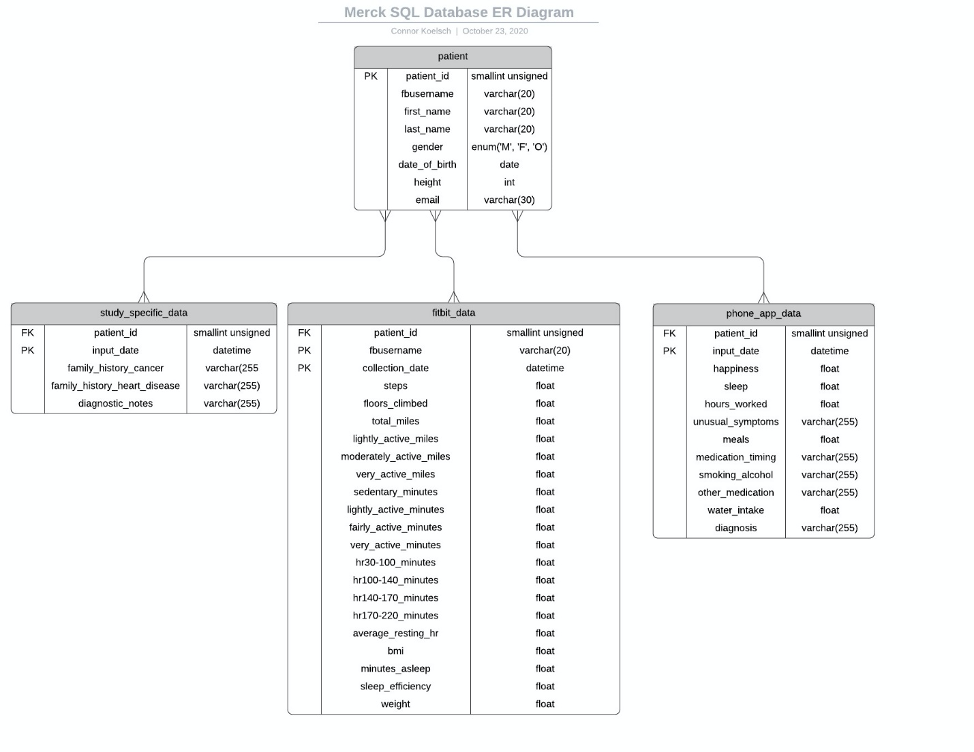
\includegraphics[width=0.50000\textwidth]{./images/entity.png}
\caption{}
\end{figure}

Database Creation with SQL Exporting the ERD above results in the
following SQL code:

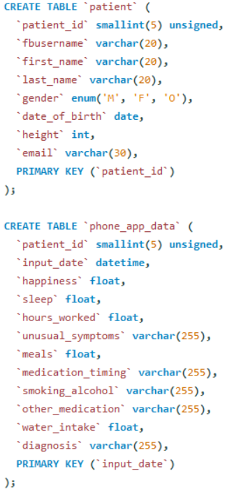
\includegraphics[width=0.40000\textwidth]{./images/a1.png}
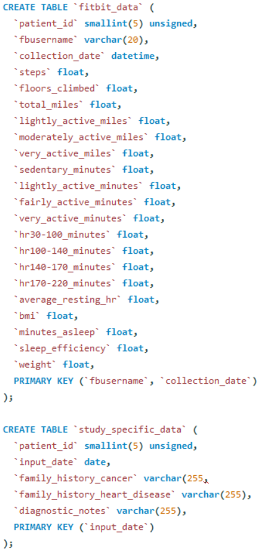
\includegraphics[width=0.40000\textwidth]{./images/a2.png}

However, this code lacks a few required pieces. The foreign keys did not
populate, and the primary keys do not reference the other tables. We
also have not ``created'' a database yet, nor told our program which
database to use. These issues are fixed in the following code snippet,
along with some syntax changes. These syntax changes were necessary
because the server our database is hosted on has some requirements that
are not very important (at least not right now).

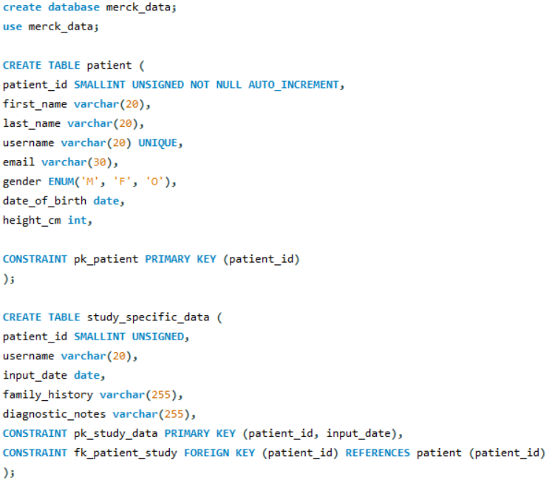
\includegraphics[width=0.50000\textwidth]{./images/a3.png}
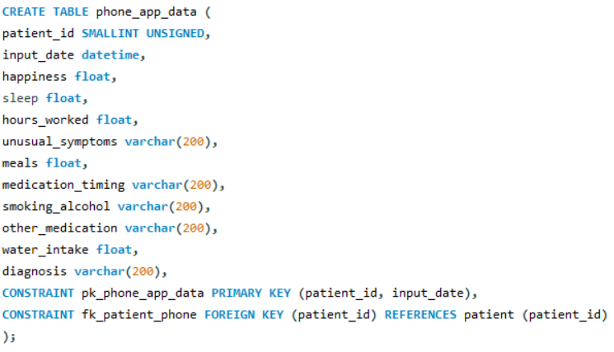
\includegraphics[width=0.50000\textwidth]{./images/a4.png}
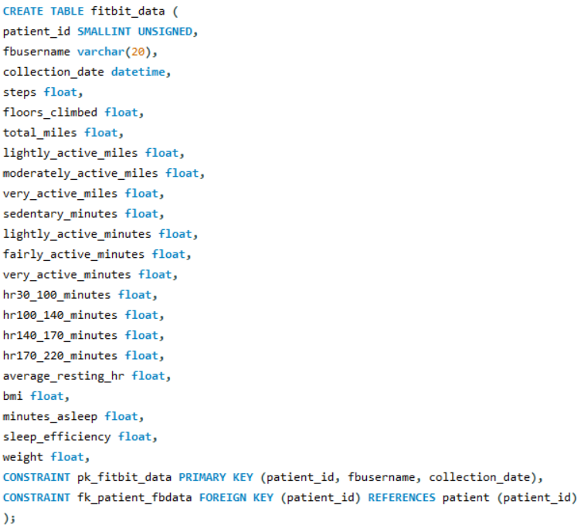
\includegraphics[width=0.50000\textwidth]{./images/a5.png}

The following snippets are useful commands for handling the database.

\begin{figure}
\centering
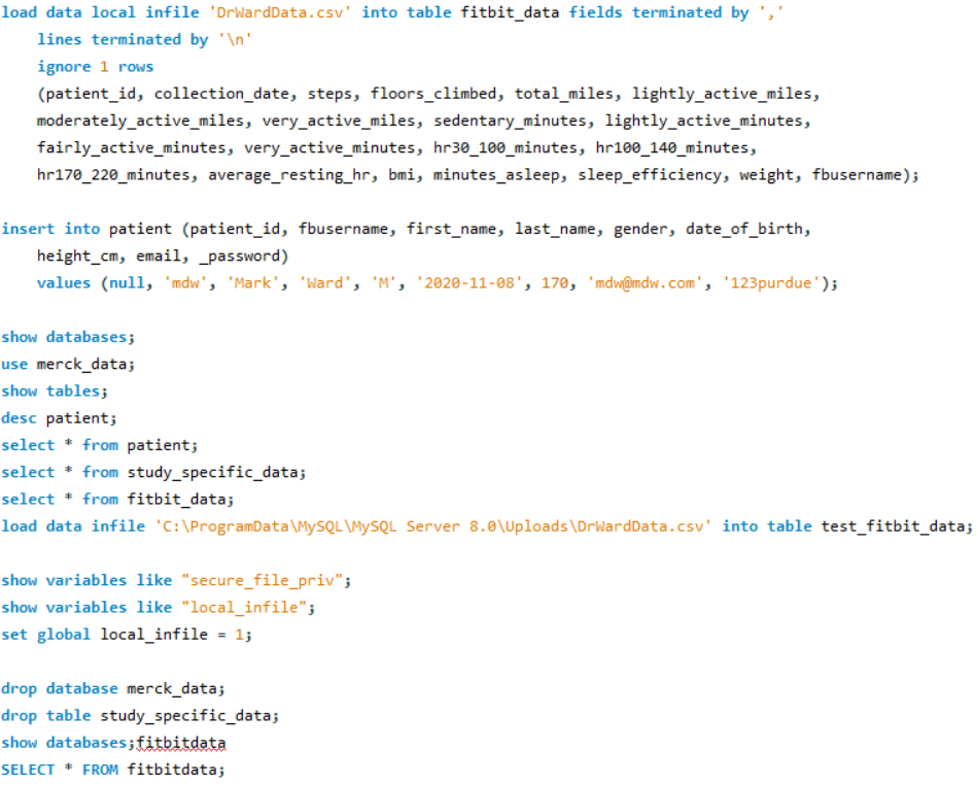
\includegraphics[width=0.50000\textwidth]{./images/a6.png}
\caption{}
\end{figure}

\section{Database Creation with
Neo4j}\label{database-creation-with-neo4j}

\subsection{Neo4j Background}\label{neo4j-background}

Neo4j is a graph database created by Neo4j inc. Neo4j is implemented in
Java; however, it can also be written with any other cypher query
language.

\section{Code}\label{code-1}

This creates the first two nodes. The yellow highlight section would be
the user node. The green highlight section shows the relationship
between the two nodes. The orange highlight section shows the other node
which would be the username. The light blue highlighted section returns
and stores the two nodes into the system.

\begin{Shaded}
\begin{Highlighting}[]
\FloatTok{1.} \KeywordTok{create}\NormalTok{(u}\OperatorTok{:}\NormalTok{user \{name}\OperatorTok{:}\StringTok{'User'}\NormalTok{\})}\OperatorTok{-}\NormalTok{[}\OperatorTok{:}\NormalTok{makes]->(n}\OperatorTok{:}\NormalTok{user\{name}\OperatorTok{:}\StringTok{'Username'}\NormalTok{\}) return u,n}
\end{Highlighting}
\end{Shaded}

The yellow highlighted section codes the user node again. Instead of
creating a new node for User we can just match the node with the new
node you want to create. The green highlighted section describes the
relationships between the two nodes. The blue highlighted section is the
code for the new node. The orange highlighted section is the code for
return which would store the nodes into the system.

\begin{Shaded}
\begin{Highlighting}[]
\FloatTok{2.} \KeywordTok{match}\NormalTok{(u}\OperatorTok{:}\NormalTok{user \{name}\OperatorTok{:}\StringTok{'User'}\NormalTok{\}) }\KeywordTok{create}\NormalTok{ (u)}\OperatorTok{-}\NormalTok{[}\OperatorTok{:}\NormalTok{enters]->}\StringTok{ }\NormalTok{(DA}\OperatorTok{:}\NormalTok{user\{name}\OperatorTok{:}\StringTok{ 'Date of Birth'}\NormalTok{\}) return u,DA}
\end{Highlighting}
\end{Shaded}

This line of code codes for a new node ``Last Name'' which stores the
last name of the patient. This node holds a relationship with the User
node.

\begin{Shaded}
\begin{Highlighting}[]
\FloatTok{3.} \KeywordTok{match}\NormalTok{(u}\OperatorTok{:}\NormalTok{user \{name}\OperatorTok{:}\StringTok{'User'}\NormalTok{\}) }\KeywordTok{create}\NormalTok{ (u)}\OperatorTok{-}\StringTok{ }\NormalTok{[}\OperatorTok{:}\NormalTok{enters]->}\StringTok{ }\NormalTok{(LN}\OperatorTok{:}\NormalTok{user\{name}\OperatorTok{:}\StringTok{'Last Name'}\NormalTok{\}) return u,LN}
\end{Highlighting}
\end{Shaded}

Similar to the code on the third line. A new node has been created,
however this node is created to store the last name of the user.

\begin{Shaded}
\begin{Highlighting}[]
\FloatTok{4.} \KeywordTok{match}\NormalTok{(u}\OperatorTok{:}\NormalTok{user \{name}\OperatorTok{:}\StringTok{'User'}\NormalTok{\}) }\KeywordTok{create}\NormalTok{ (u)}\OperatorTok{-}\StringTok{ }\NormalTok{[}\OperatorTok{:}\NormalTok{enters]->}\StringTok{ }\NormalTok{(FN}\OperatorTok{:}\NormalTok{user\{name}\OperatorTok{:}\StringTok{'First Name'}\NormalTok{\}) return u,FN}
\end{Highlighting}
\end{Shaded}

A new node is created with this code. The node stores the Height of the
user.

\begin{Shaded}
\begin{Highlighting}[]
\FloatTok{5.} \KeywordTok{match}\NormalTok{(u}\OperatorTok{:}\NormalTok{user \{name}\OperatorTok{:}\StringTok{'User'}\NormalTok{\}) }\KeywordTok{create}\NormalTok{ (u)}\OperatorTok{-}\StringTok{ }\NormalTok{[}\OperatorTok{:}\NormalTok{enters]->}\StringTok{ }\NormalTok{(H}\OperatorTok{:}\NormalTok{user\{name}\OperatorTok{:}\StringTok{'Height'}\NormalTok{\}) return u,H}
\end{Highlighting}
\end{Shaded}

The ID node is created, thus allowing for the user id to be stored.

\begin{Shaded}
\begin{Highlighting}[]
\FloatTok{6.} \KeywordTok{match}\NormalTok{(u}\OperatorTok{:}\NormalTok{user \{name}\OperatorTok{:}\StringTok{'User'}\NormalTok{\}) }\KeywordTok{create}\NormalTok{ (u)}\OperatorTok{-}\StringTok{ }\NormalTok{[}\OperatorTok{:}\NormalTok{enters]->}\StringTok{ }\NormalTok{(I}\OperatorTok{:}\NormalTok{user\{name}\OperatorTok{:}\StringTok{'ID'}\NormalTok{\}) return u,I}
\end{Highlighting}
\end{Shaded}

This line of code codes for a new node ``Merck Data'' which stores the
last name of the patient. This node holds a relationship with the ID
node.

\begin{Shaded}
\begin{Highlighting}[]
\FloatTok{7.} \KeywordTok{match}\NormalTok{(I}\OperatorTok{:}\NormalTok{user\{name}\OperatorTok{:}\StringTok{'ID'}\NormalTok{\}) }\KeywordTok{create}\NormalTok{ (I)}\OperatorTok{-}\StringTok{ }\NormalTok{[}\OperatorTok{:}\NormalTok{enters]->}\StringTok{ }\NormalTok{(M}\OperatorTok{:}\NormalTok{user\{name}\OperatorTok{:}\StringTok{'Merck Data'}\NormalTok{\}) return I,M}
\end{Highlighting}
\end{Shaded}

This line of code codes for a new node ``Family History Cancers'' which
stores the family history cancers of the patient. This node holds a
relationship with the Merck Data node.

\begin{Shaded}
\begin{Highlighting}[]
\FloatTok{8.} \KeywordTok{match}\NormalTok{(M}\OperatorTok{:}\NormalTok{user\{name}\OperatorTok{:}\StringTok{'Merck Data'}\NormalTok{\}) }\KeywordTok{create}\NormalTok{ (M)}\OperatorTok{-}\StringTok{ }\NormalTok{[}\OperatorTok{:}\NormalTok{enters]->}\StringTok{ }\NormalTok{(FH}\OperatorTok{:}\NormalTok{user\{name}\OperatorTok{:}\StringTok{'Family History Cancers'}\NormalTok{\}) return M,FH}
\end{Highlighting}
\end{Shaded}

Lines 9, 10, and 11 all code for three new nodes ``Diagnostic notes'',
`` Any other family history disease'', and ``Input Data''. This node
holds a relationship with the Merck Data node.

\begin{Shaded}
\begin{Highlighting}[]
\FloatTok{9.}  \KeywordTok{match}\NormalTok{(M}\OperatorTok{:}\NormalTok{user\{name}\OperatorTok{:}\StringTok{'Merck Data'}\NormalTok{\}) }\KeywordTok{create}\NormalTok{ (M)}\OperatorTok{-}\StringTok{ }\NormalTok{[}\OperatorTok{:}\NormalTok{enters]->}\StringTok{ }\NormalTok{(ID}\OperatorTok{:}\NormalTok{user\{name}\OperatorTok{:}\StringTok{'Input Data'}\NormalTok{\}) return M,ID}
\FloatTok{10.} \KeywordTok{match}\NormalTok{(M}\OperatorTok{:}\NormalTok{user\{name}\OperatorTok{:}\StringTok{'Merck Data'}\NormalTok{\}) }\KeywordTok{create}\NormalTok{ (M)}\OperatorTok{-}\StringTok{ }\NormalTok{[}\OperatorTok{:}\NormalTok{enters]->}\StringTok{ }\NormalTok{(DN}\OperatorTok{:}\NormalTok{user\{name}\OperatorTok{:}\StringTok{'Diagnostic Notes'}\NormalTok{\}) return M,DN}
\FloatTok{11.} \KeywordTok{match}\NormalTok{(M}\OperatorTok{:}\NormalTok{user\{name}\OperatorTok{:}\StringTok{'Merck Data'}\NormalTok{\}) }\KeywordTok{create}\NormalTok{ (M)}\OperatorTok{-}\StringTok{ }\NormalTok{[}\OperatorTok{:}\NormalTok{enters]->}\StringTok{ }\NormalTok{(AD}\OperatorTok{:}\NormalTok{user\{name}\OperatorTok{:}\StringTok{'Any other family history in disease'}\NormalTok{\}) return M,AD}
\end{Highlighting}
\end{Shaded}

This line of code helps put together all of the nodes. This is to help
you check your database while you add new nodes. This line of code will
be used throughout to double check the code, and to endure every branch
is in the correct spot.

\begin{Shaded}
\begin{Highlighting}[]
\FloatTok{12.} \KeywordTok{MATCH}\NormalTok{ (n}\OperatorTok{:}\NormalTok{user) RETURN n LIMIT }\DecValTok{100}
\end{Highlighting}
\end{Shaded}

This code creates the relationship between the node ``Username'' and the
new node ``fitbit data''. The new node will store fitbit data.

\begin{Shaded}
\begin{Highlighting}[]
\FloatTok{13.} \KeywordTok{match}\NormalTok{(n}\OperatorTok{:}\NormalTok{user\{name}\OperatorTok{:}\StringTok{'Username'}\NormalTok{\}) }\KeywordTok{create}\NormalTok{ (n)}\OperatorTok{-}\StringTok{ }\NormalTok{[}\OperatorTok{:}\NormalTok{enters]->}\StringTok{ }\NormalTok{(FD}\OperatorTok{:}\NormalTok{user\{name}\OperatorTok{:}\StringTok{'FitBit Data'}\NormalTok{\}) return n, FD}
\end{Highlighting}
\end{Shaded}

Lines 14,15,16,17,18, and 19 all create new nodes with the fit bit data
node. All the new nodes are highlighted in yellow.

\begin{Shaded}
\begin{Highlighting}[]
\FloatTok{14.} \KeywordTok{match}\NormalTok{(FD}\OperatorTok{:}\NormalTok{user\{name}\OperatorTok{:}\StringTok{'FitBit Data'}\NormalTok{\}) }\KeywordTok{create}\NormalTok{ (FD)}\OperatorTok{-}\StringTok{ }\NormalTok{[}\OperatorTok{:}\NormalTok{enters]->}\StringTok{ }\NormalTok{(WE}\OperatorTok{:}\NormalTok{user\{name}\OperatorTok{:}\StringTok{'Weight'}\NormalTok{\}) return FD,WE}
\FloatTok{15.} \KeywordTok{match}\NormalTok{(FD}\OperatorTok{:}\NormalTok{user\{name}\OperatorTok{:}\StringTok{'FitBit Data'}\NormalTok{\}) }\KeywordTok{create}\NormalTok{ (FD)}\OperatorTok{-}\StringTok{ }\NormalTok{[}\OperatorTok{:}\NormalTok{enters]->}\StringTok{ }\NormalTok{(CD}\OperatorTok{:}\NormalTok{user\{name}\OperatorTok{:}\StringTok{'Collection Date'}\NormalTok{\}) return FD,CD}
\FloatTok{16.} \KeywordTok{match}\NormalTok{(FD}\OperatorTok{:}\NormalTok{user\{name}\OperatorTok{:}\StringTok{'FitBit Data'}\NormalTok{\}) }\KeywordTok{create}\NormalTok{ (FD)}\OperatorTok{-}\StringTok{ }\NormalTok{[}\OperatorTok{:}\NormalTok{enters]->}\StringTok{ }\NormalTok{(B}\OperatorTok{:}\NormalTok{user\{name}\OperatorTok{:}\StringTok{'BMI'}\NormalTok{\}) return FD,B}
\FloatTok{17.} \KeywordTok{match}\NormalTok{(FD}\OperatorTok{:}\NormalTok{user\{name}\OperatorTok{:}\StringTok{'FitBit Data'}\NormalTok{\}) }\KeywordTok{create}\NormalTok{ (FD)}\OperatorTok{-}\StringTok{ }\NormalTok{[}\OperatorTok{:}\NormalTok{enters]->}\StringTok{ }\NormalTok{(FC}\OperatorTok{:}\NormalTok{user\{name}\OperatorTok{:}\StringTok{'Floors Climbed'}\NormalTok{\}) return FD,FC}
\FloatTok{18.} \KeywordTok{match}\NormalTok{(FD}\OperatorTok{:}\NormalTok{user\{name}\OperatorTok{:}\StringTok{'FitBit Data'}\NormalTok{\}) }\KeywordTok{create}\NormalTok{ (FD)}\OperatorTok{-}\StringTok{ }\NormalTok{[}\OperatorTok{:}\NormalTok{enters]->}\StringTok{ }\NormalTok{(ARH}\OperatorTok{:}\NormalTok{user\{name}\OperatorTok{:}\StringTok{'Average Resting Hr'}\NormalTok{\}) return FD,ARH}
\FloatTok{19.} \KeywordTok{match}\NormalTok{(FD}\OperatorTok{:}\NormalTok{user\{name}\OperatorTok{:}\StringTok{'FitBit Data'}\NormalTok{\}) }\KeywordTok{create}\NormalTok{ (FD)}\OperatorTok{-}\StringTok{ }\NormalTok{[}\OperatorTok{:}\NormalTok{enters]->}\StringTok{ }\NormalTok{(ST}\OperatorTok{:}\NormalTok{user\{name}\OperatorTok{:}\StringTok{'Steps'}\NormalTok{\}) return FD,ST}
\end{Highlighting}
\end{Shaded}

This line of code codes for a new node ``Miles'' which stores the miles
of the patient. This node holds a relationship with the Fitbit Data Node

\begin{Shaded}
\begin{Highlighting}[]
\FloatTok{20.} \KeywordTok{match}\NormalTok{(FD}\OperatorTok{:}\NormalTok{user\{name}\OperatorTok{:}\StringTok{'FitBit Data'}\NormalTok{\}) }\KeywordTok{create}\NormalTok{ (FD)}\OperatorTok{-}\StringTok{ }\NormalTok{[}\OperatorTok{:}\NormalTok{enters]->}\StringTok{ }\NormalTok{(Mi}\OperatorTok{:}\NormalTok{user\{name}\OperatorTok{:}\StringTok{'Miles'}\NormalTok{\}) return FD,Mi}
\end{Highlighting}
\end{Shaded}

Lines 20,21,22,23,24,25 all code for new nodes that hold relationships
with the Fitbit node.

\begin{Shaded}
\begin{Highlighting}[]
\FloatTok{21.} \KeywordTok{match}\NormalTok{(FD}\OperatorTok{:}\NormalTok{user\{name}\OperatorTok{:}\StringTok{'FitBit Data'}\NormalTok{\}) }\KeywordTok{create}\NormalTok{ (FD)}\OperatorTok{-}\StringTok{ }\NormalTok{[}\OperatorTok{:}\NormalTok{enters]->}\StringTok{ }\NormalTok{(TM}\OperatorTok{:}\NormalTok{user\{name}\OperatorTok{:}\StringTok{'Total Miles'}\NormalTok{\}) return FD,TM}
\FloatTok{22.} \KeywordTok{match}\NormalTok{(FD}\OperatorTok{:}\NormalTok{user\{name}\OperatorTok{:}\StringTok{'FitBit Data'}\NormalTok{\}) }\KeywordTok{create}\NormalTok{ (FD)}\OperatorTok{-}\StringTok{ }\NormalTok{[}\OperatorTok{:}\NormalTok{enters]->}\StringTok{ }\NormalTok{(VAM}\OperatorTok{:}\NormalTok{user\{name}\OperatorTok{:}\StringTok{'Very Active Miles'}\NormalTok{\}) return FD,VAM}
\FloatTok{23.} \KeywordTok{match}\NormalTok{(FD}\OperatorTok{:}\NormalTok{user\{name}\OperatorTok{:}\StringTok{'FitBit Data'}\NormalTok{\}) }\KeywordTok{create}\NormalTok{ (FD)}\OperatorTok{-}\StringTok{ }\NormalTok{[}\OperatorTok{:}\NormalTok{enters]->}\StringTok{ }\NormalTok{(LAM}\OperatorTok{:}\NormalTok{user\{name}\OperatorTok{:}\StringTok{'Lightly Active Miles'}\NormalTok{\}) return FD,LAM}
\FloatTok{24.} \KeywordTok{match}\NormalTok{(FD}\OperatorTok{:}\NormalTok{user\{name}\OperatorTok{:}\StringTok{'FitBit Data'}\NormalTok{\}) }\KeywordTok{create}\NormalTok{ (FD)}\OperatorTok{-}\StringTok{ }\NormalTok{[}\OperatorTok{:}\NormalTok{enters]->}\StringTok{ }\NormalTok{(MAM}\OperatorTok{:}\NormalTok{user\{name}\OperatorTok{:}\StringTok{'Moderately Active Miles'}\NormalTok{\}) return FD,MAM}
\FloatTok{25.} \KeywordTok{match}\NormalTok{(FD}\OperatorTok{:}\NormalTok{user\{name}\OperatorTok{:}\StringTok{'FitBit Data'}\NormalTok{\}) }\KeywordTok{create}\NormalTok{ (FD)}\OperatorTok{-}\StringTok{ }\NormalTok{[}\OperatorTok{:}\NormalTok{enters]->}\StringTok{ }\NormalTok{(S}\OperatorTok{:}\NormalTok{user\{name}\OperatorTok{:}\StringTok{'Sleep'}\NormalTok{\}) return FD,S}
\end{Highlighting}
\end{Shaded}

Lines 26,27 all codes for new nodes that holds relationships with the
``Sleep node''.

\begin{Shaded}
\begin{Highlighting}[]
\FloatTok{26.}  \KeywordTok{match}\NormalTok{(S}\OperatorTok{:}\NormalTok{user\{name}\OperatorTok{:}\StringTok{'Sleep'}\NormalTok{\}) }\KeywordTok{create}\NormalTok{ (S)}\OperatorTok{-}\StringTok{ }\NormalTok{[}\OperatorTok{:}\NormalTok{enters]->}\StringTok{ }\NormalTok{(SE}\OperatorTok{:}\NormalTok{user\{name}\OperatorTok{:}\StringTok{'Sleep Efficiency'}\NormalTok{\}) return S,SE}
\FloatTok{27.} \KeywordTok{match}\NormalTok{(S}\OperatorTok{:}\NormalTok{user\{name}\OperatorTok{:}\StringTok{'Sleep'}\NormalTok{\}) }\KeywordTok{create}\NormalTok{ (S)}\OperatorTok{-}\StringTok{ }\NormalTok{[}\OperatorTok{:}\NormalTok{enters]->}\StringTok{ }\NormalTok{(MAS}\OperatorTok{:}\NormalTok{user\{name}\OperatorTok{:}\StringTok{'Minutes Asleep'}\NormalTok{\}) return S,MAS}
\end{Highlighting}
\end{Shaded}

Lines 28,29,30,31,32,33,34,35,36 all codes for new nodes that hold
relationships with the ``minute node''.

\begin{Shaded}
\begin{Highlighting}[]
\FloatTok{28.} \KeywordTok{match}\NormalTok{(FD}\OperatorTok{:}\NormalTok{user\{name}\OperatorTok{:}\StringTok{'FitBit Data'}\NormalTok{\}) }\KeywordTok{create}\NormalTok{ (FD)}\OperatorTok{-}\StringTok{ }\NormalTok{[}\OperatorTok{:}\NormalTok{enters]->}\StringTok{ }\NormalTok{(M}\OperatorTok{:}\NormalTok{user\{name}\OperatorTok{:}\StringTok{'Minutes'}\NormalTok{\}) return FD,M}
\FloatTok{29.} \KeywordTok{match}\NormalTok{(M}\OperatorTok{:}\NormalTok{user\{name}\OperatorTok{:}\StringTok{'Minutes'}\NormalTok{\}) }\KeywordTok{create}\NormalTok{ (M)}\OperatorTok{-}\StringTok{ }\NormalTok{[}\OperatorTok{:}\NormalTok{enters]->}\StringTok{ }\NormalTok{(OF}\OperatorTok{:}\NormalTok{user\{name}\OperatorTok{:}\StringTok{'hr 140-170'}\NormalTok{\}) return M,OF}
\FloatTok{30.} \KeywordTok{match}\NormalTok{(M}\OperatorTok{:}\NormalTok{user\{name}\OperatorTok{:}\StringTok{'Minutes'}\NormalTok{\}) }\KeywordTok{create}\NormalTok{ (M)}\OperatorTok{-}\StringTok{ }\NormalTok{[}\OperatorTok{:}\NormalTok{enters]->}\StringTok{ }\NormalTok{(SM}\OperatorTok{:}\NormalTok{user\{name}\OperatorTok{:}\StringTok{'Sedentary Minutes'}\NormalTok{\}) return M,SM}
\FloatTok{31.} \KeywordTok{match}\NormalTok{(M}\OperatorTok{:}\NormalTok{user\{name}\OperatorTok{:}\StringTok{'Minutes'}\NormalTok{\}) }\KeywordTok{create}\NormalTok{ (M)}\OperatorTok{-}\StringTok{ }\NormalTok{[}\OperatorTok{:}\NormalTok{enters]->}\StringTok{ }\NormalTok{(LAM}\OperatorTok{:}\NormalTok{user\{name}\OperatorTok{:}\StringTok{'Lightly Active Minutes'}\NormalTok{\}) return M,LAM}
\FloatTok{32.} \KeywordTok{match}\NormalTok{(M}\OperatorTok{:}\NormalTok{user\{name}\OperatorTok{:}\StringTok{'Minutes'}\NormalTok{\}) }\KeywordTok{create}\NormalTok{ (M)}\OperatorTok{-}\StringTok{ }\NormalTok{[}\OperatorTok{:}\NormalTok{enters]->}\StringTok{ }\NormalTok{(FAM}\OperatorTok{:}\NormalTok{user\{name}\OperatorTok{:}\StringTok{'Fairly Active Minutes'}\NormalTok{\}) return M,FAM}
\FloatTok{33.} \KeywordTok{match}\NormalTok{(M}\OperatorTok{:}\NormalTok{user\{name}\OperatorTok{:}\StringTok{'Minutes'}\NormalTok{\}) }\KeywordTok{create}\NormalTok{ (M)}\OperatorTok{-}\StringTok{ }\NormalTok{[}\OperatorTok{:}\NormalTok{enters]->}\StringTok{ }\NormalTok{(VAM}\OperatorTok{:}\NormalTok{user\{name}\OperatorTok{:}\StringTok{'Very Active Minutes'}\NormalTok{\}) return M,VAM}
\FloatTok{34.} \KeywordTok{match}\NormalTok{(M}\OperatorTok{:}\NormalTok{user\{name}\OperatorTok{:}\StringTok{'Minutes'}\NormalTok{\}) }\KeywordTok{create}\NormalTok{ (M)}\OperatorTok{-}\StringTok{ }\NormalTok{[}\OperatorTok{:}\NormalTok{enters]->}\StringTok{ }\NormalTok{(HR}\OperatorTok{:}\NormalTok{user\{name}\OperatorTok{:}\StringTok{'hr 30-100'}\NormalTok{\}) return M,HR}
\FloatTok{35.} \KeywordTok{match}\NormalTok{(M}\OperatorTok{:}\NormalTok{user\{name}\OperatorTok{:}\StringTok{'Minutes'}\NormalTok{\}) }\KeywordTok{create}\NormalTok{ (M)}\OperatorTok{-}\StringTok{ }\NormalTok{[}\OperatorTok{:}\NormalTok{enters]->}\StringTok{ }\NormalTok{(HR1}\OperatorTok{:}\NormalTok{user\{name}\OperatorTok{:}\StringTok{'hr 100-140'}\NormalTok{\}) return M,HR1}
\FloatTok{36.} \KeywordTok{match}\NormalTok{(M}\OperatorTok{:}\NormalTok{user\{name}\OperatorTok{:}\StringTok{'Minutes'}\NormalTok{\}) }\KeywordTok{create}\NormalTok{ (M)}\OperatorTok{-}\StringTok{ }\NormalTok{[}\OperatorTok{:}\NormalTok{enters]->}\StringTok{ }\NormalTok{(HR2}\OperatorTok{:}\NormalTok{user\{name}\OperatorTok{:}\StringTok{'hr 170-220'}\NormalTok{\}) return M,HR2}
\end{Highlighting}
\end{Shaded}

Lines 37-49 all codes for new nodes that hold relationships with the
``Pain Data'' node. The highlighted portions are the new nodes.

\begin{Shaded}
\begin{Highlighting}[]
\FloatTok{37.} \KeywordTok{MATCH}\NormalTok{ (n}\OperatorTok{:}\NormalTok{user) RETURN n LIMIT }\DecValTok{100}
\FloatTok{38.} \KeywordTok{match}\NormalTok{(u}\OperatorTok{:}\NormalTok{user \{name}\OperatorTok{:}\StringTok{'User'}\NormalTok{\}) }\KeywordTok{create}\NormalTok{ (u)}\OperatorTok{-}\StringTok{ }\NormalTok{[}\OperatorTok{:}\NormalTok{enters]->}\StringTok{ }\NormalTok{(PD}\OperatorTok{:}\NormalTok{user\{name}\OperatorTok{:}\StringTok{'Pain Data'}\NormalTok{\}) return u,PD}
\FloatTok{39.} \KeywordTok{match}\NormalTok{(PD}\OperatorTok{:}\NormalTok{user\{name}\OperatorTok{:}\StringTok{'Pain Data'}\NormalTok{\}) }\KeywordTok{create}\NormalTok{ (PD)}\OperatorTok{-}\StringTok{ }\NormalTok{[}\OperatorTok{:}\NormalTok{enters]->}\StringTok{ }\NormalTok{(D}\OperatorTok{:}\NormalTok{user\{name}\OperatorTok{:}\StringTok{'Diagnosis'}\NormalTok{\}) return PD,D}
\FloatTok{40.} \KeywordTok{match}\NormalTok{(PD}\OperatorTok{:}\NormalTok{user\{name}\OperatorTok{:}\StringTok{'Pain Data'}\NormalTok{\}) }\KeywordTok{create}\NormalTok{ (PD)}\OperatorTok{-}\StringTok{ }\NormalTok{[}\OperatorTok{:}\NormalTok{enters]->}\StringTok{ }\NormalTok{(WI}\OperatorTok{:}\NormalTok{user\{name}\OperatorTok{:}\StringTok{'Water Intake'}\NormalTok{\}) return PD,WI}
\FloatTok{41.} \KeywordTok{match}\NormalTok{(PD}\OperatorTok{:}\NormalTok{user\{name}\OperatorTok{:}\StringTok{'Pain Data'}\NormalTok{\}) }\KeywordTok{create}\NormalTok{ (PD)}\OperatorTok{-}\StringTok{ }\NormalTok{[}\OperatorTok{:}\NormalTok{enters]->}\StringTok{ }\NormalTok{(MT}\OperatorTok{:}\NormalTok{user\{name}\OperatorTok{:}\StringTok{'Medication Timing'}\NormalTok{\}) return PD,MT}
\FloatTok{42.} \KeywordTok{match}\NormalTok{(PD}\OperatorTok{:}\NormalTok{user\{name}\OperatorTok{:}\StringTok{'Pain Data'}\NormalTok{\}) }\KeywordTok{create}\NormalTok{ (PD)}\OperatorTok{-}\StringTok{ }\NormalTok{[}\OperatorTok{:}\NormalTok{enters]->}\StringTok{ }\NormalTok{(DA}\OperatorTok{:}\NormalTok{user\{name}\OperatorTok{:}\StringTok{'Date'}\NormalTok{\}) return PD,DA}
\FloatTok{43.} \KeywordTok{match}\NormalTok{(PD}\OperatorTok{:}\NormalTok{user\{name}\OperatorTok{:}\StringTok{'Pain Data'}\NormalTok{\}) }\KeywordTok{create}\NormalTok{ (PD)}\OperatorTok{-}\StringTok{ }\NormalTok{[}\OperatorTok{:}\NormalTok{enters]->}\StringTok{ }\NormalTok{(HA}\OperatorTok{:}\NormalTok{user\{name}\OperatorTok{:}\StringTok{'Happiness'}\NormalTok{\}) return PD,HA}
\FloatTok{44.} \KeywordTok{match}\NormalTok{(PD}\OperatorTok{:}\NormalTok{user\{name}\OperatorTok{:}\StringTok{'Pain Data'}\NormalTok{\}) }\KeywordTok{create}\NormalTok{ (PD)}\OperatorTok{-}\StringTok{ }\NormalTok{[}\OperatorTok{:}\NormalTok{enters]->}\StringTok{ }\NormalTok{(OM}\OperatorTok{:}\NormalTok{user\{name}\OperatorTok{:}\StringTok{'Other Medication'}\NormalTok{\}) return PD,OM}
\FloatTok{45.} \KeywordTok{match}\NormalTok{(PD}\OperatorTok{:}\NormalTok{user\{name}\OperatorTok{:}\StringTok{'Pain Data'}\NormalTok{\}) }\KeywordTok{create}\NormalTok{ (PD)}\OperatorTok{-}\StringTok{ }\NormalTok{[}\OperatorTok{:}\NormalTok{enters]->}\StringTok{ }\NormalTok{(SL}\OperatorTok{:}\NormalTok{user\{name}\OperatorTok{:}\StringTok{'Sleep'}\NormalTok{\}) return PD,SL}
\FloatTok{46.} \KeywordTok{match}\NormalTok{(PD}\OperatorTok{:}\NormalTok{user\{name}\OperatorTok{:}\StringTok{'Pain Data'}\NormalTok{\}) }\KeywordTok{create}\NormalTok{ (PD)}\OperatorTok{-}\StringTok{ }\NormalTok{[}\OperatorTok{:}\NormalTok{enters]->}\StringTok{ }\NormalTok{(HW}\OperatorTok{:}\NormalTok{user\{name}\OperatorTok{:}\StringTok{'Hours Worked'}\NormalTok{\}) return PD,HW}
\FloatTok{47.} \KeywordTok{match}\NormalTok{(PD}\OperatorTok{:}\NormalTok{user\{name}\OperatorTok{:}\StringTok{'Pain Data'}\NormalTok{\}) }\KeywordTok{create}\NormalTok{ (PD)}\OperatorTok{-}\StringTok{ }\NormalTok{[}\OperatorTok{:}\NormalTok{enters]->}\StringTok{ }\NormalTok{(US}\OperatorTok{:}\NormalTok{user\{name}\OperatorTok{:}\StringTok{'Unusual Symptoms'}\NormalTok{\}) return PD,US}
\FloatTok{48.} \KeywordTok{match}\NormalTok{(PD}\OperatorTok{:}\NormalTok{user\{name}\OperatorTok{:}\StringTok{'Pain Data'}\NormalTok{\}) }\KeywordTok{create}\NormalTok{ (PD)}\OperatorTok{-}\StringTok{ }\NormalTok{[}\OperatorTok{:}\NormalTok{enters]->}\StringTok{ }\NormalTok{(M}\OperatorTok{:}\NormalTok{user\{name}\OperatorTok{:}\StringTok{'meals'}\NormalTok{\}) return PD,M}
\FloatTok{49.} \KeywordTok{match}\NormalTok{(PD}\OperatorTok{:}\NormalTok{user\{name}\OperatorTok{:}\StringTok{'Pain Data'}\NormalTok{\}) }\KeywordTok{create}\NormalTok{ (PD)}\OperatorTok{-}\StringTok{ }\NormalTok{[}\OperatorTok{:}\NormalTok{enters]->}\StringTok{ }\NormalTok{(SA}\OperatorTok{:}\NormalTok{user\{name}\OperatorTok{:}\StringTok{'Smoking/Alcohol'}\NormalTok{\}) return PD,SA}
\end{Highlighting}
\end{Shaded}

\chapter{Data visualization Team}\label{data-visualization-team}

\section{Biometric Wearables}\label{biometric-wearables}

This project is a part of the Purdue data science initiative, where
students are given an opportunity to work on the data-driven project,
guided by an industry mentor. This Biometric Wearables project is a part
of an ongoing collaboration between the Purdue and Merck industry.
Following is the brief description of the project:

\section{Purpose}\label{purpose}

The purpose of the project is to create an automated system that will
capture the biometric data from wearable fitness technology using the
mobile application and communicate its' result to Merck scientists.

\section{Outcome}\label{outcome}

This automated system will be able to collect accurate and less biased
data from the clinical trial patients because the digital process
reduces the human error and reduce the pressure on the clinical trial
patient with manual processing procedure.

\section{Significance}\label{significance}

This project may help to reduce the experiment biased by collecting more
extensive data and using the technology. Also, this approach may help to
reduce the clinical trial time and cost to ease of data collection.

\section{Overview of Data visualization
Team}\label{overview-of-data-visualization-team}

This team is a part of a big team working on the above-described
project, part of the Merck-Purdue data science collaboration. This team
has been assigned the responsibility to design rich, interactive
graphics, data visualization, and plotting method to facilitate the
MERCK scientists. In addition, this team is responsible for
brainstorming the data, and experiments with different visualization
techniques that can help the project.

\section{Previous Work Done on the
project}\label{previous-work-done-on-the-project}

The previous team that worked on the data visualization aspect of this
project created a baseline shiny website that had some specific widgets
created. There are two pages on the shiny website i.e., activity
progress and step goals. The activity progress has a bar chart that
shows the progress by comparing two biometric data points. The bar chart
has an x-axis which is to show the dates and a y-axis which is to show
the steps. One of the widget's features on this page was created to view
a specific time period of the data. The second page is to show step
goals using a pie chart.

\section{Team Members}\label{team-members}

Following is the brief introduction of the data visualization team
members:

\subsection{Ahmed Ashraf Butt}\label{ahmed-ashraf-butt}

He is a doctoral student at the School of Engineering Education, Purdue
University. He is currently working as a research assistant on the
CourseMIRROR project funded by the Institute of Education Sciences
(IES). He is interested in designing educational tools and exploring
their impact on enhancing students' learning experiences. Also, he is
working on the Merck-Purdue data science collaboration responsible for
creating an automated system that will capture the biometric data from
the wearable fitness technology using the mobile application and
communicate its result to Merck scientists.

\subsection{Pika Seth}\label{pika-seth}

She is a second-year student in the College of Engineering studying
Biomedical Engineering at Purdue University. She is currently involved
with the Data Mine Corporate Program working on the Biometrics Wearable
Project with Merck. She is involved with the data visualization aspect
dealing with the programming of R Shiny. She is a part of the Red Cross
Club and the Women in Engineering Program. Also, she is a part of the
Sigma Delta Tau sorority.

\subsection{Sharon Patta}\label{sharon-patta}

She is a first-year student in the College of Science at Purdue
University. She is studying data science. Her interests are in the
fields of AI and machine learning.

\subsection{Surya Suresh}\label{surya-suresh}

He is a first-year student in the College of Science at Purdue
University studying Computer Science. He is working with the Merck Data
Mine group on the Data Visualization part of the project.

\section{Team formation}\label{team-formation}

The team has worked together to become more familiar with R programming
and shiny application. Each member of the group explored different data
visualizations and then, worked colloborately to implement a new
visualization or improving the previous shiny app. Additionally, the
group had several meetings to collectively present findings to one
another and discuss errors and troubleshooting.

\section{Term goals}\label{term-goals}

We are going to begin working on adding more features to the old Shiny
App as well as implementing our own visualizations that we think would
be useful. We also need to figure out where we are getting our data from
once the API is running because as of right now we are just taking it
off of the CSV file that has Dr.~Ward's data.

\section{Visulization 1}\label{visulization-1}

In this visualization, we were able to create a visualization that
adapts to the given data and creates a Data Table with all of the given
data. We used the Data Tables library to accomplish this. The Data Table
contains two main tabs. One tab contains all of the mean values of the
given data. The other tab allows the user to navigate through all of the
data points in a clean and efficient way.Specifically it allows the user
to filter the data as well as list the data in any desired order. For
example, the data can be listed in order from the days with the most
steps to the days with the least. \#\#\# Code

I imported the libraries needed for the vizualization

\begin{Shaded}
\begin{Highlighting}[]
\KeywordTok{library}\NormalTok{(shiny) }\CommentTok{#Used for Shiny Dashboard}
\KeywordTok{library}\NormalTok{(ggplot2) }\CommentTok{#Needed for Plots (Not specifically this Viz)}
\KeywordTok{library}\NormalTok{(reshape2) }\CommentTok{#Needed for Plots (Not specifically this Viz)}
\KeywordTok{library}\NormalTok{(DT) }\CommentTok{#Used for the Data Tables used in this Vizualization}
\end{Highlighting}
\end{Shaded}

biometric data `bioFinal.csv' for biometric data from 2020 Feb. to
present? - Merckteam's data `DrWardData.csv' for biometric data from
2016 to 2019 April - Dr.~Ward's data

Used to read data into the myDF data frame

\begin{Shaded}
\begin{Highlighting}[]
\NormalTok{myDF <-}\StringTok{ }\KeywordTok{read.csv}\NormalTok{(}\StringTok{"liveMerck.csv"}\NormalTok{,}\OtherTok{TRUE}\NormalTok{,}\StringTok{","}\NormalTok{)}
\end{Highlighting}
\end{Shaded}

active miles (stacked)

\begin{Shaded}
\begin{Highlighting}[]
\NormalTok{miles1 <-}\StringTok{ }\KeywordTok{subset}\NormalTok{(myDF, }\DataTypeTok{select =} \KeywordTok{c}\NormalTok{(}\StringTok{'Date'}\NormalTok{,}\StringTok{'Lightly.Active.Miles'}\NormalTok{,}
                                  \StringTok{'Moderately.Active.Miles'}\NormalTok{,}
                                  \StringTok{'Very.Active.Miles'}\NormalTok{))}
\NormalTok{miles <-}\StringTok{ }\KeywordTok{melt}\NormalTok{(miles1)}
\NormalTok{miles}\OperatorTok{$}\NormalTok{Date <-}\StringTok{ }\KeywordTok{as.Date}\NormalTok{(miles}\OperatorTok{$}\NormalTok{Date)}
\end{Highlighting}
\end{Shaded}

active minutes (stacked)

\begin{Shaded}
\begin{Highlighting}[]
\NormalTok{minutes1 <-}\StringTok{ }\KeywordTok{subset}\NormalTok{(myDF, }\DataTypeTok{select =} \KeywordTok{c}\NormalTok{(}\StringTok{'Date'}\NormalTok{, }\StringTok{'Sedentary.Minutes'}\NormalTok{,}
                                    \StringTok{'Lightly.Active.Minutes'}\NormalTok{,}
                                    \StringTok{'Fairly.Active.Minutes'}\NormalTok{,}
                                    \StringTok{'Very.Active.Minutes'}\NormalTok{))}
\NormalTok{minutes <-}\StringTok{ }\KeywordTok{melt}\NormalTok{(minutes1)}
\NormalTok{minutes}\OperatorTok{$}\NormalTok{Date <-}\StringTok{ }\KeywordTok{as.Date}\NormalTok{(minutes}\OperatorTok{$}\NormalTok{Date)}
\end{Highlighting}
\end{Shaded}

HR minutes (stacked)

\begin{Shaded}
\begin{Highlighting}[]
\NormalTok{hr1 <-}\StringTok{ }\KeywordTok{subset}\NormalTok{(myDF, }\DataTypeTok{select =} \KeywordTok{c}\NormalTok{(}\StringTok{'Date'}\NormalTok{, }\StringTok{'HR.30.100.Minutes'}\NormalTok{,}
                               \StringTok{'HR.100.140.Minutes'}\NormalTok{, }\StringTok{'HR.140.170.Minutes'}\NormalTok{,}
                               \StringTok{'HR.170.220.Minutes'}\NormalTok{))}
\NormalTok{hr <-}\StringTok{ }\KeywordTok{melt}\NormalTok{(hr1)}
\NormalTok{hr}\OperatorTok{$}\NormalTok{Date <-}\StringTok{ }\KeywordTok{as.Date}\NormalTok{(hr}\OperatorTok{$}\NormalTok{Date)}
\end{Highlighting}
\end{Shaded}

Finding out the collums index with numeric value in it.

\begin{Shaded}
\begin{Highlighting}[]
\NormalTok{columsIndexWithNumberValue <-}\StringTok{ }\KeywordTok{unlist}\NormalTok{(}\KeywordTok{lapply}\NormalTok{(myDF, is.numeric)) }
\end{Highlighting}
\end{Shaded}

Extracting the columns with number value in it.

\begin{Shaded}
\begin{Highlighting}[]
\NormalTok{columWithNumber <-}\StringTok{ }\NormalTok{myDF[ , columsIndexWithNumberValue]}
\end{Highlighting}
\end{Shaded}

finding the mean of all collum's mean

\begin{Shaded}
\begin{Highlighting}[]
\NormalTok{meansOFColumWithNumber <-}\StringTok{ }\KeywordTok{lapply}\NormalTok{(columWithNumber[,], mean,}\DataTypeTok{na.rm=}\OtherTok{TRUE}\NormalTok{)}
\end{Highlighting}
\end{Shaded}

Converting them back into data frame.

\begin{Shaded}
\begin{Highlighting}[]
\NormalTok{meansOFColumWithNumberDataFrame<-}\KeywordTok{data.frame}\NormalTok{(}\KeywordTok{matrix}\NormalTok{(}\KeywordTok{unlist}\NormalTok{(meansOFColumWithNumber), }\DataTypeTok{nrow=}\KeywordTok{length}\NormalTok{(meansOFColumWithNumber), }\DataTypeTok{byrow=}\NormalTok{T))}
\end{Highlighting}
\end{Shaded}

Extracting the name of the collums names from columWithNumber.

\begin{Shaded}
\begin{Highlighting}[]
\NormalTok{colName<-}\StringTok{ }\KeywordTok{data.frame}\NormalTok{(}\KeywordTok{names}\NormalTok{(columWithNumber))}
\end{Highlighting}
\end{Shaded}

Extracting the name of the collums.

\begin{Shaded}
\begin{Highlighting}[]
\NormalTok{finalDataFrame <-}\StringTok{ }\KeywordTok{data.frame}\NormalTok{(}\DataTypeTok{a=}\NormalTok{colName, }\DataTypeTok{c=}\NormalTok{meansOFColumWithNumberDataFrame)}
\end{Highlighting}
\end{Shaded}

changing the Collum name of the final dataframe

\begin{Shaded}
\begin{Highlighting}[]
\KeywordTok{colnames}\NormalTok{(finalDataFrame)[}\DecValTok{1}\NormalTok{]<-}\StringTok{"Variables"}
\KeywordTok{colnames}\NormalTok{(finalDataFrame)[}\DecValTok{2}\NormalTok{]<-}\StringTok{"Mean Values"}
\end{Highlighting}
\end{Shaded}

myDF to date format

\begin{Shaded}
\begin{Highlighting}[]
\NormalTok{myDF}\OperatorTok{$}\NormalTok{Date =}\StringTok{ }\KeywordTok{as.Date}\NormalTok{(myDF}\OperatorTok{$}\NormalTok{Date)}
\end{Highlighting}
\end{Shaded}

Remove the X column from myDF

\begin{Shaded}
\begin{Highlighting}[]
\NormalTok{drops <-}\StringTok{ }\KeywordTok{c}\NormalTok{(}\StringTok{"X"}\NormalTok{)}
\NormalTok{myDF <-}\StringTok{ }\NormalTok{myDF[ , }\OperatorTok{!}\NormalTok{(}\KeywordTok{names}\NormalTok{(myDF) }\OperatorTok\StringTok{ }\NormalTok{drops)]}
\end{Highlighting}
\end{Shaded}

UI of the Application

\begin{Shaded}
\begin{Highlighting}[]
\CommentTok{# Uses the fluidPage and a Sidebar Layout}
\NormalTok{ui <-}\StringTok{ }\KeywordTok{fluidPage}\NormalTok{(}
  \DataTypeTok{title =} \StringTok{"Tester"}\NormalTok{,}
  \KeywordTok{titlePanel}\NormalTok{(}\StringTok{"Visualization 1"}\NormalTok{),}
  \KeywordTok{sidebarLayout}\NormalTok{(}
    \KeywordTok{sidebarPanel}\NormalTok{(}
      \CommentTok{# This panel contains the first Data Table}
      \KeywordTok{conditionalPanel}\NormalTok{(}
        \CommentTok{#input.dataset is used in DT's to show which data is actually used}
        \StringTok{'input.dataset === "myDF"'}\NormalTok{,}
        \CommentTok{#Included a checkbox for what columns should be in the data Table}
        \CommentTok{#The pre selected columns are "Date" and "Steps"}
        \KeywordTok{checkboxGroupInput}\NormalTok{(}\StringTok{"show_vars"}\NormalTok{, }\StringTok{"Columns of information to show:"}\NormalTok{,}
                           \KeywordTok{names}\NormalTok{(myDF), }\DataTypeTok{selected =} \KeywordTok{list}\NormalTok{(}\StringTok{"Date"}\NormalTok{, }\StringTok{"Steps"}\NormalTok{))}
\NormalTok{      ),}
      \CommentTok{# This panel contains the second Data Table}
      \KeywordTok{conditionalPanel}\NormalTok{(}
        \CommentTok{#input.dataset is used in DT's to show which data is actually used}
        \StringTok{'input.dataset === "finalDataFrame"'}\NormalTok{,}
        \CommentTok{#We can change this text to anything we want user to see}
        \KeywordTok{helpText}\NormalTok{(}\StringTok{"Click the column header to sort a column."}\NormalTok{)}
\NormalTok{      ),}
\NormalTok{    ),}
    \KeywordTok{mainPanel}\NormalTok{(}
      \CommentTok{# Allows the user to pick between the 2 tabs containing the Data Tables}
      \KeywordTok{tabsetPanel}\NormalTok{(}
        \CommentTok{#name of the tabs}
        \DataTypeTok{id =} \StringTok{'dataset'}\NormalTok{,}
        \CommentTok{#First tab named "myDF" contains Data Table from first set of data}
        \KeywordTok{tabPanel}\NormalTok{(}\StringTok{"myDF"}\NormalTok{, DT}\OperatorTok{::}\KeywordTok{dataTableOutput}\NormalTok{(}\StringTok{"mytable1"}\NormalTok{)),}
        \CommentTok{#Second tab named "finalDataFrame" contains DT from second set of data}
        \KeywordTok{tabPanel}\NormalTok{(}\StringTok{"finalDataFrame"}\NormalTok{, DT}\OperatorTok{::}\KeywordTok{dataTableOutput}\NormalTok{(}\StringTok{"mytable2"}\NormalTok{))}
\NormalTok{      )}
\NormalTok{    )}
\NormalTok{  )}
\NormalTok{)}
\end{Highlighting}
\end{Shaded}

Server of the Application

\begin{Shaded}
\begin{Highlighting}[]
\NormalTok{server <-}\StringTok{ }\ControlFlowTok{function}\NormalTok{(input, output) \{}
  \CommentTok{# choose columns to display}
\NormalTok{  myDF2 =}\StringTok{ }\NormalTok{myDF[}\KeywordTok{sample}\NormalTok{(}\KeywordTok{nrow}\NormalTok{(myDF), }\KeywordTok{nrow}\NormalTok{(myDF), }\DataTypeTok{replace =} \OtherTok{FALSE}\NormalTok{), ]}
  \CommentTok{#Used to render the actual Data Table based off any changes made by the user}
  \CommentTok{#Changes based on what variables are selected and the filter feature is}
  \CommentTok{#located on the top of the Data Table}
\NormalTok{  output}\OperatorTok{$}\NormalTok{mytable1 <-}\StringTok{ }\NormalTok{DT}\OperatorTok{::}\KeywordTok{renderDataTable}\NormalTok{(\{}
\NormalTok{    DT}\OperatorTok{::}\KeywordTok{datatable}\NormalTok{(myDF2[, input}\OperatorTok{$}\NormalTok{show_vars, }\DataTypeTok{drop =} \OtherTok{FALSE}\NormalTok{], }\DataTypeTok{rownames =} \OtherTok{FALSE}\NormalTok{, }\DataTypeTok{filter =} \StringTok{'top'}\NormalTok{)}
\NormalTok{  \})}
  
  \CommentTok{#Used to render teh Data Table and does not have many features like the first}
  \CommentTok{#Data Table. This one only contains the means (finalDataFrame)}
\NormalTok{  output}\OperatorTok{$}\NormalTok{mytable2 <-}\StringTok{ }\NormalTok{DT}\OperatorTok{::}\KeywordTok{renderDataTable}\NormalTok{(\{}
\NormalTok{    DT}\OperatorTok{::}\KeywordTok{datatable}\NormalTok{(finalDataFrame, }\DataTypeTok{options =} \KeywordTok{list}\NormalTok{(}\DataTypeTok{orderClasses =} \OtherTok{TRUE}\NormalTok{), }\DataTypeTok{rownames =} \OtherTok{FALSE}\NormalTok{)}
\NormalTok{  \})}
\NormalTok{\}}
\end{Highlighting}
\end{Shaded}

Runs the application

\begin{Shaded}
\begin{Highlighting}[]
\KeywordTok{shinyApp}\NormalTok{(ui, server)}
\end{Highlighting}
\end{Shaded}

\section{Visulization 2}\label{visulization-2}

In this visulization, we categorizes the data into three categories:
Steps and Floors Climbed, Distance, and Activity Level. Each category
contains bar graphs that display the data for each respective variable
per month. Both the Distance and the Activity Level categories display
visualizations that separate the data into different subcategories based
on the intensity of the activity.

\subsection{Code}\label{code-2}

\begin{Shaded}
\begin{Highlighting}[]
\KeywordTok{library}\NormalTok{(shiny)}
\KeywordTok{library}\NormalTok{(ggplot2)}
\KeywordTok{library}\NormalTok{(reshape2)}
\CommentTok{# biometric data}
\CommentTok{# 'bioFinal.csv' for biometric data from 2020 Feb. to present? - Merckteam's data}
\CommentTok{# 'DrWardData.csv' for biometric data from 2016 to 2019 April - Dr. Ward's data}

\CommentTok{#This function reads in the CSV file that contains the data, named DrWardData.csv, and stores it in a data frame called myDF. The argument for the read.csv function is the path where the CSV file is located.}
\NormalTok{myDF <-}\StringTok{ }\KeywordTok{read.csv}\NormalTok{(}\StringTok{"/class/datamine/corporate/merck/Merck201920/fitbit_data/DrWardData.csv"}\NormalTok{)}

\CommentTok{# The subset function selects the data from the myDF data frame that separates the miles the user has walked by activity level, as well as the date column. This subset is stored as "miles1".}
\CommentTok{# The melt function then takes the columns stored in miles1 and stacks them into a single column in "miles".}
\CommentTok{# The as.Date function goes into the Date column of "miles" and correctly formats the values as a date.}
\NormalTok{miles1 <-}\StringTok{ }\KeywordTok{subset}\NormalTok{(myDF, }\DataTypeTok{select =} \KeywordTok{c}\NormalTok{(}\StringTok{'Date'}\NormalTok{,}\StringTok{'Lightly.Active.Miles'}\NormalTok{, }\StringTok{'Moderately.Active.Miles'}\NormalTok{, }\StringTok{'Very.Active.Miles'}\NormalTok{))}
\NormalTok{miles <-}\StringTok{ }\KeywordTok{melt}\NormalTok{(miles1)}
\NormalTok{miles}\OperatorTok{$}\NormalTok{Date <-}\StringTok{ }\KeywordTok{as.Date}\NormalTok{(miles}\OperatorTok{$}\NormalTok{Date)}

\CommentTok{# The subset function selects the data from the myDF data frame that separates the minutes the user spends in activity by activity level, as well as the date column. This subset is stored as "minutes1".}
\CommentTok{# The melt function then takes the columns stored in minutes1 and stacks them into a single column in "minutes".}
\CommentTok{# The as.Date function goes into the Date column of "minutes" and correctly formats the values as a date.}
\NormalTok{minutes1 <-}\StringTok{ }\KeywordTok{subset}\NormalTok{(myDF, }\DataTypeTok{select =} \KeywordTok{c}\NormalTok{(}\StringTok{'Date'}\NormalTok{, }\StringTok{'Sedentary.Minutes'}\NormalTok{, }\StringTok{'Lightly.Active.Minutes'}\NormalTok{, }\StringTok{'Fairly.Active.Minutes'}\NormalTok{, }\StringTok{'Very.Active.Minutes'}\NormalTok{))}
\NormalTok{minutes <-}\StringTok{ }\KeywordTok{melt}\NormalTok{(minutes1)}
\NormalTok{minutes}\OperatorTok{$}\NormalTok{Date <-}\StringTok{ }\KeywordTok{as.Date}\NormalTok{(minutes}\OperatorTok{$}\NormalTok{Date)}

\CommentTok{# The subset function selects the data from the myDF data frame that separates the data by the number of minutes the user spent with heart rate between 30-100 bpm, 100-140 bpm, 140-170 bpm, and 170-220 bpm, as well as the date column. This subset is stored as "hr1".}
\CommentTok{# The melt function then takes the columns stored in hr1 and stacks them into a single column in "hr".}
\CommentTok{# The as.Date function goes into the Date column of "hr" and correctly formats the values as a date.}
\NormalTok{hr1 <-}\StringTok{ }\KeywordTok{subset}\NormalTok{(myDF, }\DataTypeTok{select =} \KeywordTok{c}\NormalTok{(}\StringTok{'Date'}\NormalTok{, }\StringTok{'HR.30.100.Minutes'}\NormalTok{, }\StringTok{'HR.100.140.Minutes'}\NormalTok{, }\StringTok{'HR.140.170.Minutes'}\NormalTok{, }\StringTok{'HR.170.220.Minutes'}\NormalTok{))}
\NormalTok{hr <-}\StringTok{ }\KeywordTok{melt}\NormalTok{(hr1)}
\NormalTok{hr}\OperatorTok{$}\NormalTok{Date <-}\StringTok{ }\KeywordTok{as.Date}\NormalTok{(hr}\OperatorTok{$}\NormalTok{Date)}

\CommentTok{# The as.Date function goes into the Date column of "myDF" and correctly formats the values as a date.}
\CommentTok{# The first format function goes into the year column of "myDF" and formats the values as a year.}
\CommentTok{# The second format function goes into the month column of "myDF" and formats the values as unabbreviated month names.}
\NormalTok{myDF}\OperatorTok{$}\NormalTok{Date =}\StringTok{ }\KeywordTok{as.Date}\NormalTok{(myDF}\OperatorTok{$}\NormalTok{Date)}
\NormalTok{myDF}\OperatorTok{$}\NormalTok{year <-}\StringTok{ }\KeywordTok{format}\NormalTok{(myDF}\OperatorTok{$}\NormalTok{Date,}\StringTok{'%Y'}\NormalTok{)}
\NormalTok{myDF}\OperatorTok{$}\NormalTok{month <-}\StringTok{ }\KeywordTok{factor}\NormalTok{(}\KeywordTok{format}\NormalTok{(myDF}\OperatorTok{$}\NormalTok{Date,}\StringTok{'%B'}\NormalTok{), }\DataTypeTok{levels =}\NormalTok{ month.name)}

\CommentTok{# Every shiny app must include a UI header beginning with fluidPage()}
\CommentTok{# fluidPage() allows the user to adjust the size of their window while preserving the dimensions of the display}
\NormalTok{ui<-}\KeywordTok{fluidPage}\NormalTok{(}
  \CommentTok{# The first section of code uses the navbarPage() function to create the menu at the top of the page titled “Fitbit Dashboard” that allows the user to select the “How to Use” page, the “Activity Progress” page, or the “Step Goals” page}
  
  \CommentTok{# Creates a menu of selections titled "Fitbit Dashboard"}
  \KeywordTok{navbarPage}\NormalTok{(}\StringTok{"Fitbit Dashboard"}\NormalTok{,          }
             \CommentTok{# tabPanel 1}
             
             \CommentTok{# The tabPanel() function creates the “How to Use” tab in the Fitbit Dashboard and includes the images, displays, and texts to be shown on the page}
             \KeywordTok{tabPanel}\NormalTok{(}\StringTok{"How to Use"}\NormalTok{,}
                      \CommentTok{# Includes Merck logo}
                      \KeywordTok{img}\NormalTok{(}\DataTypeTok{src =} \StringTok{"https://assets.phenompeople.com/CareerConnectResources/MERCUS/social/1200x630-1552902977090.jpg"}\NormalTok{, }\DataTypeTok{height =} \DecValTok{120}\NormalTok{, }\DataTypeTok{width =} \DecValTok{220}\NormalTok{),}
                      \CommentTok{# Creates main title "Biometric Data Dashboard"}
                      \KeywordTok{h1}\NormalTok{(}\StringTok{"Biometric Data Dashboard"}\NormalTok{),}
                      \KeywordTok{mainPanel}\NormalTok{(}
                        \CommentTok{# Includes bolded text and link}
                        \KeywordTok{strong}\NormalTok{(}\StringTok{"Refer to the website here for more information:"}\NormalTok{),}
                        \KeywordTok{a}\NormalTok{(}\StringTok{"https://www.merck.com/index.html"}\NormalTok{),}
                        \CommentTok{# Smaller heading than h1 to create title "How to Use My Dashboard"}
                        \KeywordTok{h3}\NormalTok{(}\StringTok{"How to Use My Dashboard"}\NormalTok{),}
                        \CommentTok{# Outputs HTML "text2" which is included in the server block}
                        \KeywordTok{htmlOutput}\NormalTok{(}\StringTok{"text2"}\NormalTok{)}
\NormalTok{                      )                      }
\NormalTok{             ), }
             
             \CommentTok{# tabPanel 2}
             
             \CommentTok{# The tabPanel() function creates the “Activity Progress” tab in the Fitbit Dashboard and includes the images, displays, and texts to be shown on the page}
             \KeywordTok{tabPanel}\NormalTok{(}\StringTok{"Activity Progress"}\NormalTok{,}
                      \KeywordTok{sidebarLayout}\NormalTok{(}
                        \CommentTok{# Creates title "Activity Progress" for sidebar panel}
                        \KeywordTok{sidebarPanel}\NormalTok{(}\KeywordTok{h3}\NormalTok{(}\StringTok{"Activity Progress"}\NormalTok{),}
                                     \CommentTok{# Allows user to input date range}
                                     \KeywordTok{dateRangeInput}\NormalTok{(}\StringTok{"dates"}\NormalTok{, (}\StringTok{"Date range"}\NormalTok{)),}
                                     \CommentTok{# Allows user to select single y-axis variable for graph}
                                     \KeywordTok{varSelectInput}\NormalTok{(}\StringTok{"variables"}\NormalTok{, (}\StringTok{"Variable:"}\NormalTok{), myDF[}\KeywordTok{c}\NormalTok{(}\OperatorTok{-}\DecValTok{1}\NormalTok{, }\DecValTok{-2}\NormalTok{)]),}
                                     \CommentTok{# Allows user to select variable y-axis (includes all levels of selected on the same graph)}
                                     \KeywordTok{selectInput}\NormalTok{(}\StringTok{"stack"}\NormalTok{, (}\StringTok{"Variable (Stacked):"}\NormalTok{),}
                                                 \KeywordTok{c}\NormalTok{(}\StringTok{"N/A"}\NormalTok{ =}\StringTok{ "nana"}\NormalTok{, }\StringTok{"Active Miles"}\NormalTok{ =}\StringTok{ "miles"}\NormalTok{, }\StringTok{"Active minutes"}\NormalTok{ =}\StringTok{ "minutes"}\NormalTok{, }\StringTok{"HR minutes"}\NormalTok{ =}\StringTok{ "hr"}\NormalTok{)),}
\NormalTok{                        ),}
                        \CommentTok{# Creates the main panel}
                        \KeywordTok{mainPanel}\NormalTok{(}
                          \CommentTok{# Includes italicized text}
                          \KeywordTok{em}\NormalTok{(}\StringTok{"Select a date range and a variable!"}\NormalTok{),}
                          \CommentTok{# Includes bolded text}
                          \KeywordTok{strong}\NormalTok{(}\StringTok{"Refer to the website here for more information:"}\NormalTok{),}
                          \CommentTok{# Includes link}
                          \KeywordTok{a}\NormalTok{(}\StringTok{"https://www.merck.com/index.html"}\NormalTok{),}
                          \CommentTok{# Displays the bar graph with selected variable}
                          \KeywordTok{plotOutput}\NormalTok{(}\DataTypeTok{outputId =} \StringTok{"bioBarGraph"}\NormalTok{)}
\NormalTok{                        )}
\NormalTok{                      )}
\NormalTok{             ), }
             
             \CommentTok{# tabPanel 3}
             
             \CommentTok{# The tabPanel() function creates the “Step Goals” tab in the Fitbit Dashboard and includes the images, displays, and texts to be shown on the page}
             \KeywordTok{tabPanel}\NormalTok{(}\StringTok{"Step Goals"}\NormalTok{,}
                      \CommentTok{# Creates sidebar panel with smaller heading "10,000-Step Goal"}
                      \KeywordTok{sidebarPanel}\NormalTok{(}\KeywordTok{h3}\NormalTok{(}\StringTok{"10,000-Step Goal"}\NormalTok{),}
                                   \CommentTok{# Allows user to input one specific date}
                                   \KeywordTok{dateInput}\NormalTok{(}\StringTok{"goaldate"}\NormalTok{, (}\StringTok{"Date"}\NormalTok{))}
\NormalTok{                      ),}
                      \CommentTok{# Creates the main panel}
                      \KeywordTok{mainPanel}\NormalTok{(}
                        \CommentTok{# Includes bolded text}
                        \KeywordTok{strong}\NormalTok{(}\StringTok{"Refer to the website here for more information:"}\NormalTok{),}
                        \CommentTok{# Includes link}
                        \KeywordTok{a}\NormalTok{(}\StringTok{"https://www.merck.com/index.html"}\NormalTok{),}
                        \CommentTok{# Displays pie chart}
                        \KeywordTok{plotOutput}\NormalTok{(}\DataTypeTok{outputId =} \StringTok{"bioDoughnut"}\NormalTok{)}
\NormalTok{                      )}
\NormalTok{             ),}
             \CommentTok{# tabPanel 4}
             
             \CommentTok{# The tabPanel() function creates the “Visualization 2” tab in the Fitbit Dashboard and includes the images, displays, and texts to be shown on the page}
             \KeywordTok{tabPanel}\NormalTok{(}\StringTok{"Visualization 2"}\NormalTok{,}
                      \KeywordTok{sidebarLayout}\NormalTok{(}
                        \CommentTok{# Creates title "Activity Progress" for sidebar panel}
                        \KeywordTok{sidebarPanel}\NormalTok{(}\KeywordTok{h3}\NormalTok{(}\StringTok{"Visualization 2"}\NormalTok{),}
\NormalTok{                        ),}
                        \CommentTok{# Creates the main panel}
                        \KeywordTok{mainPanel}\NormalTok{(}
                          \CommentTok{# Includes bolded text}
                          \KeywordTok{strong}\NormalTok{(}\KeywordTok{HTML}\NormalTok{(}\StringTok{"Activity graphs are listed below <br/>"}\NormalTok{)),}
                          \KeywordTok{strong}\NormalTok{(}\StringTok{"Steps and Floors Climbed"}\NormalTok{),}
                          \CommentTok{# Displays the bar graph that shows total steps per month}
                          \KeywordTok{plotOutput}\NormalTok{(}\DataTypeTok{outputId =} \StringTok{"bioStep"}\NormalTok{),}
                          \CommentTok{# Displays the bar graph that shows total floors climbed per month}
                          \KeywordTok{plotOutput}\NormalTok{(}\DataTypeTok{outputId =} \StringTok{"bioFloors"}\NormalTok{),}
                          \CommentTok{# Includes bolded text}
                          \KeywordTok{strong}\NormalTok{(}\KeywordTok{HTML}\NormalTok{(}\StringTok{"Distance <br/>"}\NormalTok{)),}
                          \CommentTok{# Includes italicized text}
                          \KeywordTok{em}\NormalTok{(}\StringTok{"This section shows the total distance walked per month in miles, as well as a breakdown of the activity level of the distance walked."}\NormalTok{),}
                          \CommentTok{# Displays the bar graph that shows total miles walked per month}
                          \KeywordTok{plotOutput}\NormalTok{(}\DataTypeTok{outputId =} \StringTok{"bioTM"}\NormalTok{),}
                          \CommentTok{# Displays the bar graph that shows total number of lightly active miles walked per month}
                          \KeywordTok{plotOutput}\NormalTok{(}\DataTypeTok{outputId =} \StringTok{"bioLM"}\NormalTok{),}
                          \CommentTok{# Displays the bar graph that shows total number of moderately active miles walked per month}
                          \KeywordTok{plotOutput}\NormalTok{(}\DataTypeTok{outputId =} \StringTok{"bioMM"}\NormalTok{),}
                          \CommentTok{# Displays the bar graph that shows total number of very active miles walked per month}
                          \KeywordTok{plotOutput}\NormalTok{(}\DataTypeTok{outputId =} \StringTok{"bioVM"}\NormalTok{),}
                          \CommentTok{# Includes bolded text}
                          \KeywordTok{strong}\NormalTok{(}\KeywordTok{HTML}\NormalTok{(}\StringTok{"Activity Level <br/>"}\NormalTok{)),}
                          \CommentTok{# Includes italicized text}
                          \KeywordTok{em}\NormalTok{(}\StringTok{"This section shows the time spent in each level of activity."}\NormalTok{),}
                          \CommentTok{# Displays the bar graph that shows the amount of time spent being lightly active per month}
                          \KeywordTok{plotOutput}\NormalTok{(}\DataTypeTok{outputId =} \StringTok{"bioLA"}\NormalTok{),}
                          \CommentTok{# Displays the bar graph that shows the amount of time spent being fairly active per month}
                          \KeywordTok{plotOutput}\NormalTok{(}\DataTypeTok{outputId =} \StringTok{"bioFA"}\NormalTok{),}
                          \CommentTok{# Displays the bar graph that shows the amount of time spent being very active per month}
                          \KeywordTok{plotOutput}\NormalTok{(}\DataTypeTok{outputId =} \StringTok{"bioVA"}\NormalTok{),}
\NormalTok{                        )}
\NormalTok{                      )}
\NormalTok{             )}
\NormalTok{  )}
\NormalTok{)}

              
\NormalTok{server <-}\StringTok{ }\ControlFlowTok{function}\NormalTok{(input, output) \{}
  
  \CommentTok{# You can access the values of the widget (as a vector of Dates)}
  \CommentTok{# with input$dates, }
  \CommentTok{# e.g. output$value <- renderPrint(\{ input$dates \})}
  
  \CommentTok{# text on tabPanel 1 }
\NormalTok{  output}\OperatorTok{$}\NormalTok{text2 <-}\StringTok{ }\KeywordTok{renderUI}\NormalTok{(\{    }
    \KeywordTok{HTML}\NormalTok{(}\KeywordTok{paste}\NormalTok{(}\StringTok{""}\NormalTok{, }\StringTok{"1. Activity Progress with Bar Charts"}\NormalTok{,}
               \StringTok{"- Date Range: select a start and an end date to set a date range of the activity progress"}\NormalTok{,}
               \StringTok{"- Variables: use the drop-down to select a variable of the activity progress you wish to see"}\NormalTok{,}
               \StringTok{"- Variables (Stacked): use the drop-down to select a variable of the activity progress you wish to see as a stacked bar chart"}\NormalTok{,}
               \StringTok{""}\NormalTok{, }\StringTok{"2. Step Goals with Doughnut Charts"}\NormalTok{, }
               \StringTok{"- Date: select a date of the activity progress you wish to see"}\NormalTok{,}
               \DataTypeTok{sep=}\StringTok{"<br/>"}\NormalTok{))}
\NormalTok{  \})}
  
  \CommentTok{# bar charts on tabPanel 2}
\NormalTok{  output}\OperatorTok{$}\NormalTok{bioBarGraph <-}\StringTok{ }\KeywordTok{renderPlot}\NormalTok{(\{}
    
    \CommentTok{# counter for the start date - date range}
\NormalTok{    counter1 =}\StringTok{ }\DecValTok{0}
    \ControlFlowTok{for}\NormalTok{ (myDate }\ControlFlowTok{in} \KeywordTok{as.character}\NormalTok{(myDF}\OperatorTok{$}\NormalTok{Date))\{}
\NormalTok{      counter1 =}\StringTok{ }\NormalTok{counter1 }\OperatorTok{+}\StringTok{ }\DecValTok{1}
      \ControlFlowTok{if}\NormalTok{ (myDate }\OperatorTok{==}\StringTok{ }\NormalTok{input}\OperatorTok{$}\NormalTok{dates[}\DecValTok{1}\NormalTok{]) \{}
        \ControlFlowTok{break}
\NormalTok{      \}}
\NormalTok{    \}}
    
    \CommentTok{# counter for the end date - date range}
\NormalTok{    counter2 =}\StringTok{ }\DecValTok{0}
    \ControlFlowTok{for}\NormalTok{ (myDate }\ControlFlowTok{in} \KeywordTok{as.character}\NormalTok{(myDF}\OperatorTok{$}\NormalTok{Date))\{}
\NormalTok{      counter2 =}\StringTok{ }\NormalTok{counter2 }\OperatorTok{+}\StringTok{ }\DecValTok{1}
      \ControlFlowTok{if}\NormalTok{ (myDate }\OperatorTok{==}\StringTok{ }\NormalTok{input}\OperatorTok{$}\NormalTok{dates[}\DecValTok{2}\NormalTok{]) \{}
        \ControlFlowTok{break}
\NormalTok{      \}}
\NormalTok{    \}}
    
    \CommentTok{# subset of myDF with the selected date range}
\NormalTok{    mySubset <-}\StringTok{ }\NormalTok{myDF[}\KeywordTok{c}\NormalTok{(counter1}\OperatorTok{:}\NormalTok{counter2),]    }
    \ControlFlowTok{if}\NormalTok{ (input}\OperatorTok{$}\NormalTok{stack }\OperatorTok{==}\StringTok{ "nana"}\NormalTok{)\{ }\CommentTok{# single bar chart - if stacked bar is N/A}
      \KeywordTok{ggplot}\NormalTok{(}\DataTypeTok{data=}\NormalTok{mySubset, }\KeywordTok{aes}\NormalTok{(}\DataTypeTok{x=}\NormalTok{Date, }\DataTypeTok{y=}\OperatorTok{!!}\NormalTok{input}\OperatorTok{$}\NormalTok{variables)) }\OperatorTok{+}\StringTok{ }\KeywordTok{geom_bar}\NormalTok{(}\DataTypeTok{stat=}\StringTok{"identity"}\NormalTok{, }\DataTypeTok{width =} \FloatTok{.5}\NormalTok{, }\DataTypeTok{fill =} \StringTok{"#13A999"}\NormalTok{)}
\NormalTok{    \}}\ControlFlowTok{else} \ControlFlowTok{if}\NormalTok{(input}\OperatorTok{$}\NormalTok{stack }\OperatorTok{==}\StringTok{ "miles"}\NormalTok{)\{ }\CommentTok{# stacked bar chart - active miles}
      \KeywordTok{ggplot}\NormalTok{(}\DataTypeTok{data=}\NormalTok{miles, }\KeywordTok{aes}\NormalTok{(}\DataTypeTok{x=}\NormalTok{Date, }\DataTypeTok{y=}\NormalTok{value, }\DataTypeTok{fill=}\NormalTok{variable)) }\OperatorTok{+}\StringTok{ }\KeywordTok{geom_bar}\NormalTok{(}\DataTypeTok{stat=}\StringTok{"identity"}\NormalTok{, }\DataTypeTok{width =} \FloatTok{.5}\NormalTok{)}
\NormalTok{    \}}\ControlFlowTok{else} \ControlFlowTok{if}\NormalTok{(input}\OperatorTok{$}\NormalTok{stack }\OperatorTok{==}\StringTok{ "minutes"}\NormalTok{)\{ }\CommentTok{# stacked bar chart - active minutes}
      \KeywordTok{ggplot}\NormalTok{(}\DataTypeTok{data=}\NormalTok{minutes, }\KeywordTok{aes}\NormalTok{(}\DataTypeTok{x=}\NormalTok{Date, }\DataTypeTok{y=}\NormalTok{value, }\DataTypeTok{fill=}\NormalTok{variable)) }\OperatorTok{+}\StringTok{ }\KeywordTok{geom_bar}\NormalTok{(}\DataTypeTok{stat=}\StringTok{"identity"}\NormalTok{, }\DataTypeTok{width =} \FloatTok{.5}\NormalTok{)}
\NormalTok{    \}}\ControlFlowTok{else} \ControlFlowTok{if}\NormalTok{(input}\OperatorTok{$}\NormalTok{stack }\OperatorTok{==}\StringTok{ "hr"}\NormalTok{)\{ }\CommentTok{# stacked bar chart - HR minutes}
      \KeywordTok{ggplot}\NormalTok{(}\DataTypeTok{data=}\NormalTok{hr, }\KeywordTok{aes}\NormalTok{(}\DataTypeTok{x=}\NormalTok{Date, }\DataTypeTok{y=}\NormalTok{value, }\DataTypeTok{fill=}\NormalTok{variable)) }\OperatorTok{+}\StringTok{ }\KeywordTok{geom_bar}\NormalTok{(}\DataTypeTok{stat=}\StringTok{"identity"}\NormalTok{, }\DataTypeTok{width =} \FloatTok{.5}\NormalTok{)}
\NormalTok{    \}}
\NormalTok{  \})}
  \CommentTok{# Visualization 2}
  \CommentTok{# Bar graph that shows total steps per month}
\NormalTok{  output}\OperatorTok{$}\NormalTok{bioStep <-}\StringTok{ }\KeywordTok{renderPlot}\NormalTok{(\{}
    \KeywordTok{ggplot}\NormalTok{(}\DataTypeTok{data =}\NormalTok{ myDF, }\KeywordTok{aes}\NormalTok{(}\DataTypeTok{x =}\NormalTok{ month, }\DataTypeTok{y=}\NormalTok{ Steps))}\OperatorTok{+}
\StringTok{      }\KeywordTok{geom_bar}\NormalTok{(}\DataTypeTok{stat =} \StringTok{"identity"}\NormalTok{, }\DataTypeTok{color =} \StringTok{"#007a73"}\NormalTok{, }\DataTypeTok{width =} \FloatTok{0.5}\NormalTok{, }\DataTypeTok{position =} \KeywordTok{position_dodge}\NormalTok{(}\DataTypeTok{width =} \FloatTok{0.6}\NormalTok{), }\DataTypeTok{fill =} \StringTok{"#007a73"}\NormalTok{) }\OperatorTok{+}
\StringTok{      }\KeywordTok{ggtitle}\NormalTok{(}\StringTok{"Total Steps per Month"}\NormalTok{) }\OperatorTok{+}
\StringTok{      }\KeywordTok{xlab}\NormalTok{(}\StringTok{"Month"}\NormalTok{) }\OperatorTok{+}
\StringTok{      }\KeywordTok{ylab}\NormalTok{(}\StringTok{"Steps"}\NormalTok{)}
\NormalTok{  \})}
  
  \CommentTok{# Bar graph that shows total floors climbed per month}
\NormalTok{  output}\OperatorTok{$}\NormalTok{bioFloors <-}\StringTok{ }\KeywordTok{renderPlot}\NormalTok{(\{}
    \KeywordTok{ggplot}\NormalTok{(}\DataTypeTok{data =}\NormalTok{ myDF, }\KeywordTok{aes}\NormalTok{(}\DataTypeTok{x =}\NormalTok{ month, }\DataTypeTok{y=}\NormalTok{ Floors.Climbed))}\OperatorTok{+}
\StringTok{      }\KeywordTok{geom_bar}\NormalTok{(}\DataTypeTok{stat =} \StringTok{"identity"}\NormalTok{, }\DataTypeTok{color =} \StringTok{"#007a73"}\NormalTok{, }\DataTypeTok{width =} \FloatTok{0.5}\NormalTok{, }\DataTypeTok{position =} \KeywordTok{position_dodge}\NormalTok{(}\DataTypeTok{width =} \FloatTok{0.6}\NormalTok{), }\DataTypeTok{fill =} \StringTok{"#007a73"}\NormalTok{) }\OperatorTok{+}
\StringTok{      }\KeywordTok{ggtitle}\NormalTok{(}\StringTok{"Total Floors Climbed per Month"}\NormalTok{) }\OperatorTok{+}
\StringTok{      }\KeywordTok{xlab}\NormalTok{(}\StringTok{"Month"}\NormalTok{) }\OperatorTok{+}
\StringTok{      }\KeywordTok{ylab}\NormalTok{(}\StringTok{"Floors Climbed"}\NormalTok{)}
\NormalTok{  \})}
  
  \CommentTok{# Bar graph that shows total miles walked per month}
\NormalTok{  output}\OperatorTok{$}\NormalTok{bioTM <-}\StringTok{ }\KeywordTok{renderPlot}\NormalTok{(\{}
    \KeywordTok{ggplot}\NormalTok{(}\DataTypeTok{data =}\NormalTok{ myDF, }\KeywordTok{aes}\NormalTok{(}\DataTypeTok{x =}\NormalTok{ month, }\DataTypeTok{y=}\NormalTok{ Total.Miles))}\OperatorTok{+}
\StringTok{      }\KeywordTok{geom_bar}\NormalTok{(}\DataTypeTok{stat =} \StringTok{"identity"}\NormalTok{, }\DataTypeTok{color =} \StringTok{"#007a73"}\NormalTok{, }\DataTypeTok{width =} \FloatTok{0.5}\NormalTok{, }\DataTypeTok{position =} \KeywordTok{position_dodge}\NormalTok{(}\DataTypeTok{width =} \FloatTok{0.6}\NormalTok{), }\DataTypeTok{fill =} \StringTok{"#007a73"}\NormalTok{) }\OperatorTok{+}
\StringTok{      }\KeywordTok{ggtitle}\NormalTok{(}\StringTok{"Total Miles Walked per Month"}\NormalTok{) }\OperatorTok{+}
\StringTok{      }\KeywordTok{xlab}\NormalTok{(}\StringTok{"Month"}\NormalTok{) }\OperatorTok{+}
\StringTok{      }\KeywordTok{ylab}\NormalTok{(}\StringTok{"Miles"}\NormalTok{)}
\NormalTok{  \})}
  
  \CommentTok{# Bar graph that shows lightly active miles walked per month}
\NormalTok{  output}\OperatorTok{$}\NormalTok{bioLM <-}\StringTok{ }\KeywordTok{renderPlot}\NormalTok{(\{}
    \KeywordTok{ggplot}\NormalTok{(}\DataTypeTok{data =}\NormalTok{ myDF, }\KeywordTok{aes}\NormalTok{(}\DataTypeTok{x =}\NormalTok{ month, }\DataTypeTok{y=}\NormalTok{ Lightly.Active.Miles))}\OperatorTok{+}
\StringTok{      }\KeywordTok{geom_bar}\NormalTok{(}\DataTypeTok{stat =} \StringTok{"identity"}\NormalTok{, }\DataTypeTok{color =} \StringTok{"#007a73"}\NormalTok{, }\DataTypeTok{width =} \FloatTok{0.5}\NormalTok{, }\DataTypeTok{position =} \KeywordTok{position_dodge}\NormalTok{(}\DataTypeTok{width =} \FloatTok{0.6}\NormalTok{), }\DataTypeTok{fill =} \StringTok{"#007a73"}\NormalTok{) }\OperatorTok{+}
\StringTok{      }\KeywordTok{ggtitle}\NormalTok{(}\StringTok{"Lightly Active Miles Walked per Month"}\NormalTok{) }\OperatorTok{+}
\StringTok{      }\KeywordTok{xlab}\NormalTok{(}\StringTok{"Month"}\NormalTok{) }\OperatorTok{+}
\StringTok{      }\KeywordTok{ylab}\NormalTok{(}\StringTok{"Miles"}\NormalTok{)}
\NormalTok{  \})}
  
  \CommentTok{# Bar graph that shows moderately active miles walked per month}
\NormalTok{  output}\OperatorTok{$}\NormalTok{bioMM <-}\StringTok{ }\KeywordTok{renderPlot}\NormalTok{(\{}
    \KeywordTok{ggplot}\NormalTok{(}\DataTypeTok{data =}\NormalTok{ myDF, }\KeywordTok{aes}\NormalTok{(}\DataTypeTok{x =}\NormalTok{ month, }\DataTypeTok{y=}\NormalTok{ Moderately.Active.Miles))}\OperatorTok{+}
\StringTok{      }\KeywordTok{geom_bar}\NormalTok{(}\DataTypeTok{stat =} \StringTok{"identity"}\NormalTok{, }\DataTypeTok{color =} \StringTok{"#007a73"}\NormalTok{, }\DataTypeTok{width =} \FloatTok{0.5}\NormalTok{, }\DataTypeTok{position =} \KeywordTok{position_dodge}\NormalTok{(}\DataTypeTok{width =} \FloatTok{0.6}\NormalTok{), }\DataTypeTok{fill =} \StringTok{"#007a73"}\NormalTok{) }\OperatorTok{+}
\StringTok{      }\KeywordTok{ggtitle}\NormalTok{(}\StringTok{"Moderately Active Miles Walked per Month"}\NormalTok{) }\OperatorTok{+}
\StringTok{      }\KeywordTok{xlab}\NormalTok{(}\StringTok{"Month"}\NormalTok{) }\OperatorTok{+}
\StringTok{      }\KeywordTok{ylab}\NormalTok{(}\StringTok{"Miles"}\NormalTok{)}
\NormalTok{  \})}
  
  \CommentTok{# Bar graph that shows very active miles walked per month}
\NormalTok{  output}\OperatorTok{$}\NormalTok{bioVM <-}\StringTok{ }\KeywordTok{renderPlot}\NormalTok{(\{}
    \KeywordTok{ggplot}\NormalTok{(}\DataTypeTok{data =}\NormalTok{ myDF, }\KeywordTok{aes}\NormalTok{(}\DataTypeTok{x =}\NormalTok{ month, }\DataTypeTok{y=}\NormalTok{ Very.Active.Miles))}\OperatorTok{+}
\StringTok{      }\KeywordTok{geom_bar}\NormalTok{(}\DataTypeTok{stat =} \StringTok{"identity"}\NormalTok{, }\DataTypeTok{color =} \StringTok{"#007a73"}\NormalTok{, }\DataTypeTok{width =} \FloatTok{0.5}\NormalTok{, }\DataTypeTok{position =} \KeywordTok{position_dodge}\NormalTok{(}\DataTypeTok{width =} \FloatTok{0.6}\NormalTok{), }\DataTypeTok{fill =} \StringTok{"#007a73"}\NormalTok{) }\OperatorTok{+}
\StringTok{      }\KeywordTok{ggtitle}\NormalTok{(}\StringTok{"Very Active Miles Walked per Month"}\NormalTok{) }\OperatorTok{+}
\StringTok{      }\KeywordTok{xlab}\NormalTok{(}\StringTok{"Month"}\NormalTok{) }\OperatorTok{+}
\StringTok{      }\KeywordTok{ylab}\NormalTok{(}\StringTok{"Miles"}\NormalTok{)}
\NormalTok{  \})}
  
  \CommentTok{# Bar graph that shows the amount of time spent being lightly active per month}
\NormalTok{  output}\OperatorTok{$}\NormalTok{bioLA <-}\StringTok{ }\KeywordTok{renderPlot}\NormalTok{(\{}
    \KeywordTok{ggplot}\NormalTok{(}\DataTypeTok{data =}\NormalTok{ myDF, }\KeywordTok{aes}\NormalTok{(}\DataTypeTok{x =}\NormalTok{ month, }\DataTypeTok{y=}\NormalTok{ Lightly.Active.Minutes))}\OperatorTok{+}
\StringTok{      }\KeywordTok{geom_bar}\NormalTok{(}\DataTypeTok{stat =} \StringTok{"identity"}\NormalTok{, }\DataTypeTok{color =} \StringTok{"#007a73"}\NormalTok{, }\DataTypeTok{width =} \FloatTok{0.5}\NormalTok{, }\DataTypeTok{position =} \KeywordTok{position_dodge}\NormalTok{(}\DataTypeTok{width =} \FloatTok{0.6}\NormalTok{), }\DataTypeTok{fill =} \StringTok{"#007a73"}\NormalTok{) }\OperatorTok{+}
\StringTok{      }\KeywordTok{ggtitle}\NormalTok{(}\StringTok{"Time Spent Being Lightly Active per Month"}\NormalTok{) }\OperatorTok{+}
\StringTok{      }\KeywordTok{xlab}\NormalTok{(}\StringTok{"Month"}\NormalTok{) }\OperatorTok{+}
\StringTok{      }\KeywordTok{ylab}\NormalTok{(}\StringTok{"Minutes"}\NormalTok{)}
\NormalTok{  \})}
  
  \CommentTok{# Bar graph that shows the amount of time spent being fairly active per month}
\NormalTok{  output}\OperatorTok{$}\NormalTok{bioFA <-}\StringTok{ }\KeywordTok{renderPlot}\NormalTok{(\{}
    \KeywordTok{ggplot}\NormalTok{(}\DataTypeTok{data =}\NormalTok{ myDF, }\KeywordTok{aes}\NormalTok{(}\DataTypeTok{x =}\NormalTok{ month, }\DataTypeTok{y=}\NormalTok{ Fairly.Active.Minutes))}\OperatorTok{+}
\StringTok{      }\KeywordTok{geom_bar}\NormalTok{(}\DataTypeTok{stat =} \StringTok{"identity"}\NormalTok{, }\DataTypeTok{color =} \StringTok{"#007a73"}\NormalTok{, }\DataTypeTok{width =} \FloatTok{0.5}\NormalTok{, }\DataTypeTok{position =} \KeywordTok{position_dodge}\NormalTok{(}\DataTypeTok{width =} \FloatTok{0.6}\NormalTok{), }\DataTypeTok{fill =} \StringTok{"#007a73"}\NormalTok{) }\OperatorTok{+}
\StringTok{      }\KeywordTok{ggtitle}\NormalTok{(}\StringTok{"Time Spent Being Fairly Active per Month"}\NormalTok{) }\OperatorTok{+}
\StringTok{      }\KeywordTok{xlab}\NormalTok{(}\StringTok{"Month"}\NormalTok{) }\OperatorTok{+}
\StringTok{      }\KeywordTok{ylab}\NormalTok{(}\StringTok{"Minutes"}\NormalTok{)}
\NormalTok{  \})}
  
  \CommentTok{# Bar graph that shows the amount of time spent being very active per month}
\NormalTok{  output}\OperatorTok{$}\NormalTok{bioVA <-}\StringTok{ }\KeywordTok{renderPlot}\NormalTok{(\{}
    \KeywordTok{ggplot}\NormalTok{(}\DataTypeTok{data =}\NormalTok{ myDF, }\KeywordTok{aes}\NormalTok{(}\DataTypeTok{x =}\NormalTok{ month, }\DataTypeTok{y=}\NormalTok{ Very.Active.Minutes))}\OperatorTok{+}
\StringTok{      }\KeywordTok{geom_bar}\NormalTok{(}\DataTypeTok{stat =} \StringTok{"identity"}\NormalTok{, }\DataTypeTok{color =} \StringTok{"#007a73"}\NormalTok{, }\DataTypeTok{width =} \FloatTok{0.5}\NormalTok{, }\DataTypeTok{position =} \KeywordTok{position_dodge}\NormalTok{(}\DataTypeTok{width =} \FloatTok{0.6}\NormalTok{), }\DataTypeTok{fill =} \StringTok{"#007a73"}\NormalTok{) }\OperatorTok{+}
\StringTok{      }\KeywordTok{ggtitle}\NormalTok{(}\StringTok{"Time Spent Being Very Active per Month"}\NormalTok{) }\OperatorTok{+}
\StringTok{      }\KeywordTok{xlab}\NormalTok{(}\StringTok{"Month"}\NormalTok{) }\OperatorTok{+}
\StringTok{      }\KeywordTok{ylab}\NormalTok{(}\StringTok{"Minutes"}\NormalTok{)}
\NormalTok{  \})}
  
  
  \CommentTok{# doughnut chart on tabPanel 3}
\NormalTok{  output}\OperatorTok{$}\NormalTok{bioDoughnut <-}\StringTok{ }\KeywordTok{renderPlot}\NormalTok{(\{}
    
    \CommentTok{# counter for the date - daily goals}
\NormalTok{    counter3 =}\StringTok{ }\DecValTok{0} 
    \ControlFlowTok{for}\NormalTok{ (myDate }\ControlFlowTok{in} \KeywordTok{as.character}\NormalTok{(myDF}\OperatorTok{$}\NormalTok{Date))\{}
\NormalTok{      counter3 =}\StringTok{ }\NormalTok{counter3 }\OperatorTok{+}\StringTok{ }\DecValTok{1}
      \ControlFlowTok{if}\NormalTok{ (myDate }\OperatorTok{==}\StringTok{ }\NormalTok{input}\OperatorTok{$}\NormalTok{goaldate) \{}
        \ControlFlowTok{break}
\NormalTok{      \}}
\NormalTok{    \}}
    
    \CommentTok{# doughnut bar}
    \CommentTok{# daily steps of the selected date}
\NormalTok{    steps <-}\StringTok{ }\NormalTok{myDF[}\KeywordTok{c}\NormalTok{(counter3}\OperatorTok{:}\NormalTok{counter3),}\KeywordTok{c}\NormalTok{(}\StringTok{"Steps"}\NormalTok{)]}
    \CommentTok{# get a percentage - daily steps out of 10000 steps}
\NormalTok{    data <-}\StringTok{ }\KeywordTok{data.frame}\NormalTok{(}
      \DataTypeTok{category=}\KeywordTok{c}\NormalTok{(}\StringTok{"Steps"}\NormalTok{,}\StringTok{"N/A"}\NormalTok{),}
      \DataTypeTok{count=}\KeywordTok{c}\NormalTok{(steps, }\DecValTok{10000}\OperatorTok{-}\NormalTok{steps)}
\NormalTok{    )}
\NormalTok{    data}\OperatorTok{$}\NormalTok{fraction =}\StringTok{ }\NormalTok{data}\OperatorTok{$}\NormalTok{count }\OperatorTok{/}\StringTok{ }\DecValTok{100}
\NormalTok{    data}\OperatorTok{$}\NormalTok{ymax =}\StringTok{ }\KeywordTok{cumsum}\NormalTok{(data}\OperatorTok{$}\NormalTok{fraction)}
\NormalTok{    data}\OperatorTok{$}\NormalTok{ymin =}\StringTok{ }\KeywordTok{c}\NormalTok{(}\DecValTok{0}\NormalTok{, }\KeywordTok{head}\NormalTok{(data}\OperatorTok{$}\NormalTok{ymax, }\DataTypeTok{n=}\OperatorTok{-}\DecValTok{1}\NormalTok{))}
    \KeywordTok{ggplot}\NormalTok{(data, }\KeywordTok{aes}\NormalTok{(}\DataTypeTok{ymax=}\NormalTok{ymax, }\DataTypeTok{ymin=}\NormalTok{ymin, }\DataTypeTok{xmax=}\DecValTok{4}\NormalTok{, }\DataTypeTok{xmin=}\DecValTok{3}\NormalTok{, }\DataTypeTok{fill=}\NormalTok{category)) }\OperatorTok{+}\StringTok{ }\KeywordTok{geom_rect}\NormalTok{() }\OperatorTok{+}\StringTok{ }\KeywordTok{coord_polar}\NormalTok{(}\DataTypeTok{theta=}\StringTok{"y"}\NormalTok{) }\OperatorTok{+}\StringTok{ }\KeywordTok{xlim}\NormalTok{(}\KeywordTok{c}\NormalTok{(}\DecValTok{2}\NormalTok{, }\DecValTok{4}\NormalTok{))}
\NormalTok{  \})}
\NormalTok{\}}
\KeywordTok{shinyApp}\NormalTok{(ui, server)}
\end{Highlighting}
\end{Shaded}

\section{Critical decisions}\label{critical-decisions}

Our group decided to use RStudio to test pieces of R code on our own
local machines, but we ran into the problem of not being able to
collaborate with our team in an efficient way, so we looked for an
alternative method where we could all have access to update a file. We
decided to create a repository on bitbucket where we all had access to
the files and could update everything using git.

After setting up the colloboration, we started working to improve the
previous dashboard and implementing new feature. To improve our skills
in R shiny dashboard, we each implemented a different form of data
visualization, including a histogram, a scatterplot, a box plot, and a
pie chart, and implemented them using data from the previous year.
Additionally, we looked at code from the previous year's team and tried
to run their app and resolve any issues that occurred.

While implementing the visulization, we faced few difficuluties. For
instance, in the viuslization 1, we have to modify the whole
visualization as our initial visulization was having issue to modify
itself during the user interaction. Simialarly, second visulization was
interactive initially and allowed the user to choose which variable they
wanted to see on the graph. However, an issue we faced with this was
that when the user selected a variable, the values on the y-axis would
become N/A and the bars on the graph would all be the same height. After
discussing several potential solutions to this issue, we decided that
the best option would be to create several static graphs, allowing the
user to scroll to the desired graph.

\section{Technical Report}\label{technical-report-1}

During the last sprint, we focused mainly on the visualization and
refinement stages of our development process. In the visualization
stage, we brainstormed, discussed, and developed the code for the two
visualizations we created. In the refinement stage, we reviewed the
issues in the code and discussed potential solutions. We then cycled
back to the visualization stage in order to implement the solutions we
discussed.

\chapter{Back End Team}\label{back-end-team}

\section{Creation of Dummy Data}\label{creation-of-dummy-data}

\subsection{Why do we need dummy data?}\label{why-do-we-need-dummy-data}

In order to effectively test the functionality of the backend code, a
lot of pre-existing data is needed to fill the database to simulate a
normal functioning environment for the app. Initially, we only had about
40 users' data, and it was not enough. Therefore, we decided to create
fake user data based on pre-existing user data (dummy data).

\subsection{How we generated dummy
data?}\label{how-we-generated-dummy-data}

In order to let dummy data make sense and follow pre-existing data's
patterns, we studied the patterns of each pre-existing data category.
There are active, basal, dist, elev, heart, and steps data. We mostly
used user 185 and 186's dataset as the reference while creating dummy
dataset.

For the active data, we first calculated the mean value of the original
data. Then we found out the number of data points above the mean.
Because it can be observed that within each active data set, data points
above the mean value cluster into three group, and one of them always
starts at the beginning. Therefore, we also chose the start as the
position of the first high value data cluster, and randomly chose
position for the other two. The value of each data point was chosen
based on the observed range of the reference data point.

The result of fake data vs.~real data graph can be found below:\\
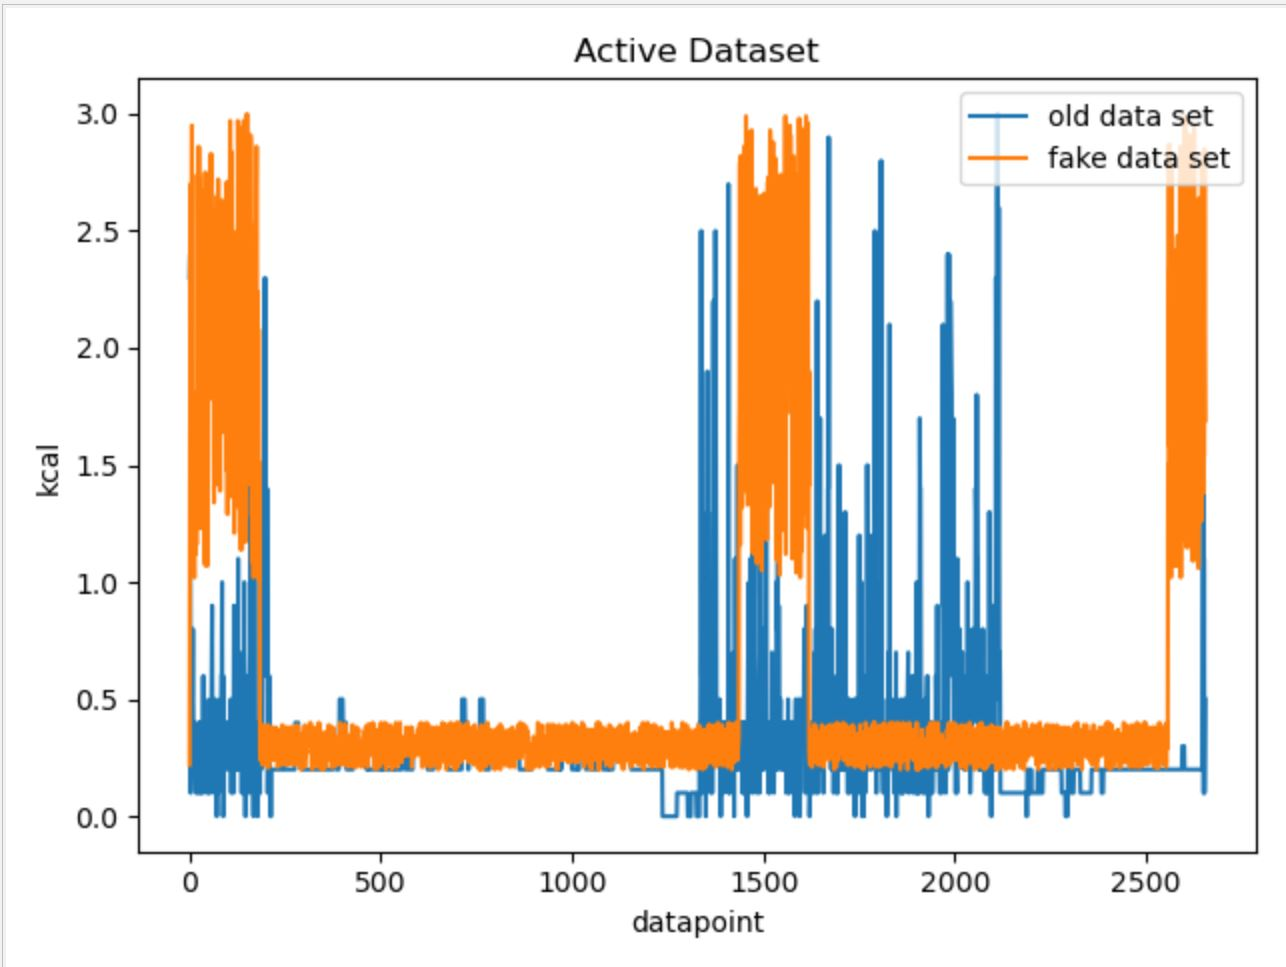
\includegraphics[width=0.50000\textwidth]{./images/Active Data.JPG}

For other data categories, we utilized similar approaches while ajusting
parameters and the possible range of random number generation based on
each data categories' own characteristics. Below are the fake data
vs.~real data comparison graphs for other data categories.

For basal data:\\
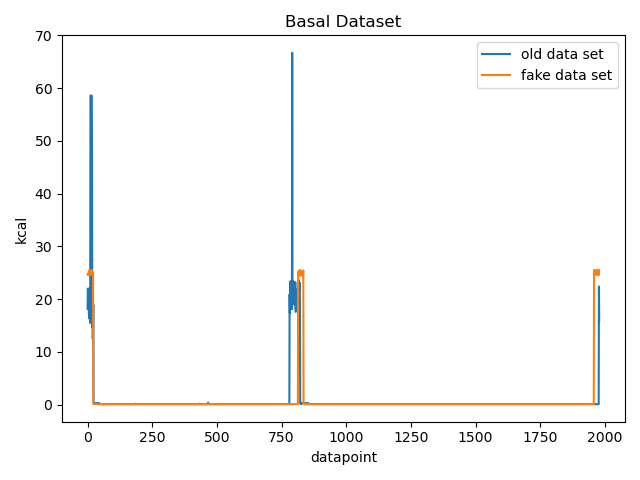
\includegraphics[width=0.50000\textwidth]{./images/BasalData.png} For
Dist data:\\
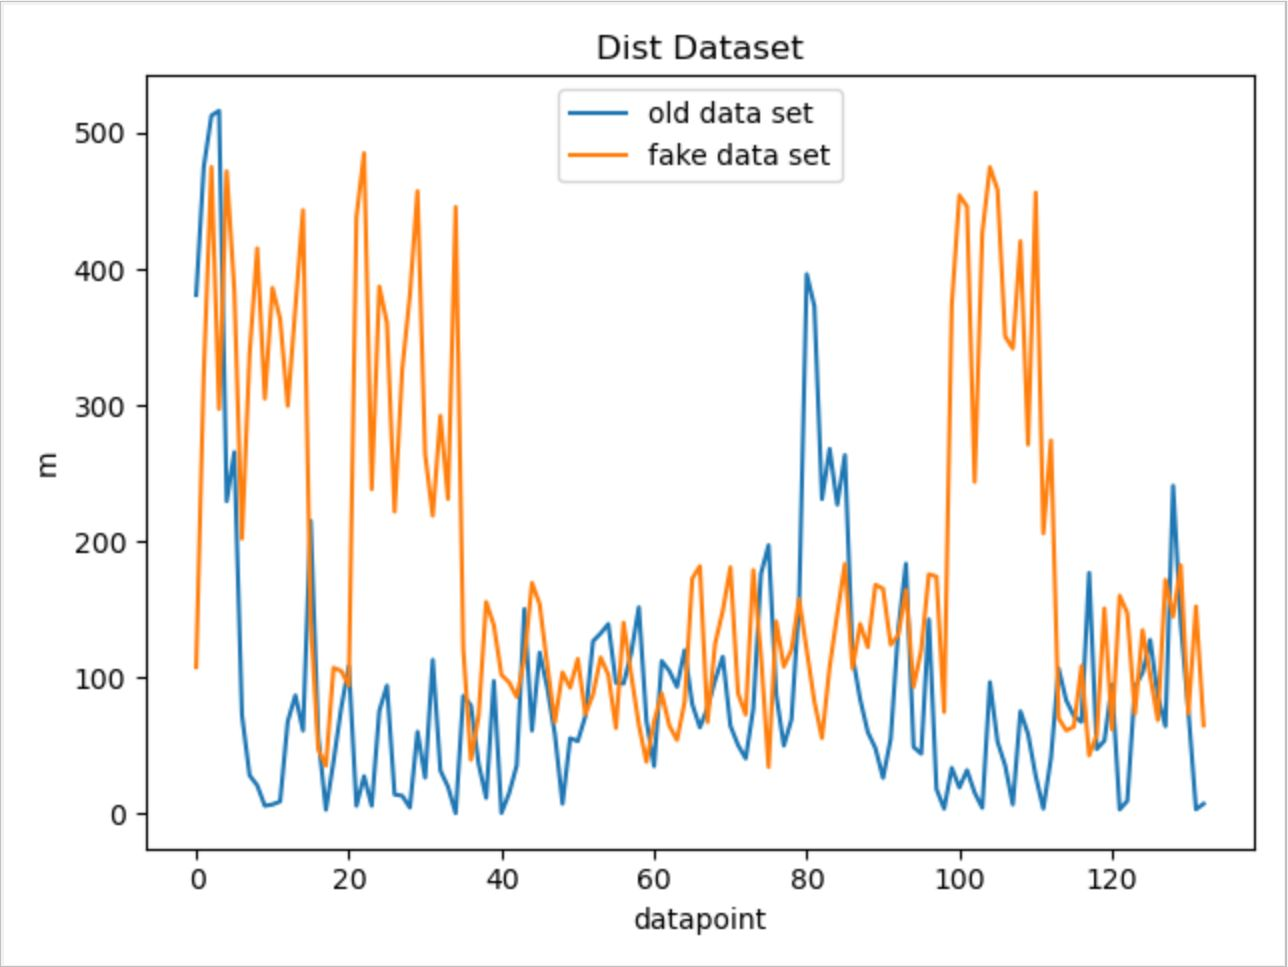
\includegraphics[width=0.50000\textwidth]{./images/Dist Data.JPG} For
Elev data:\\
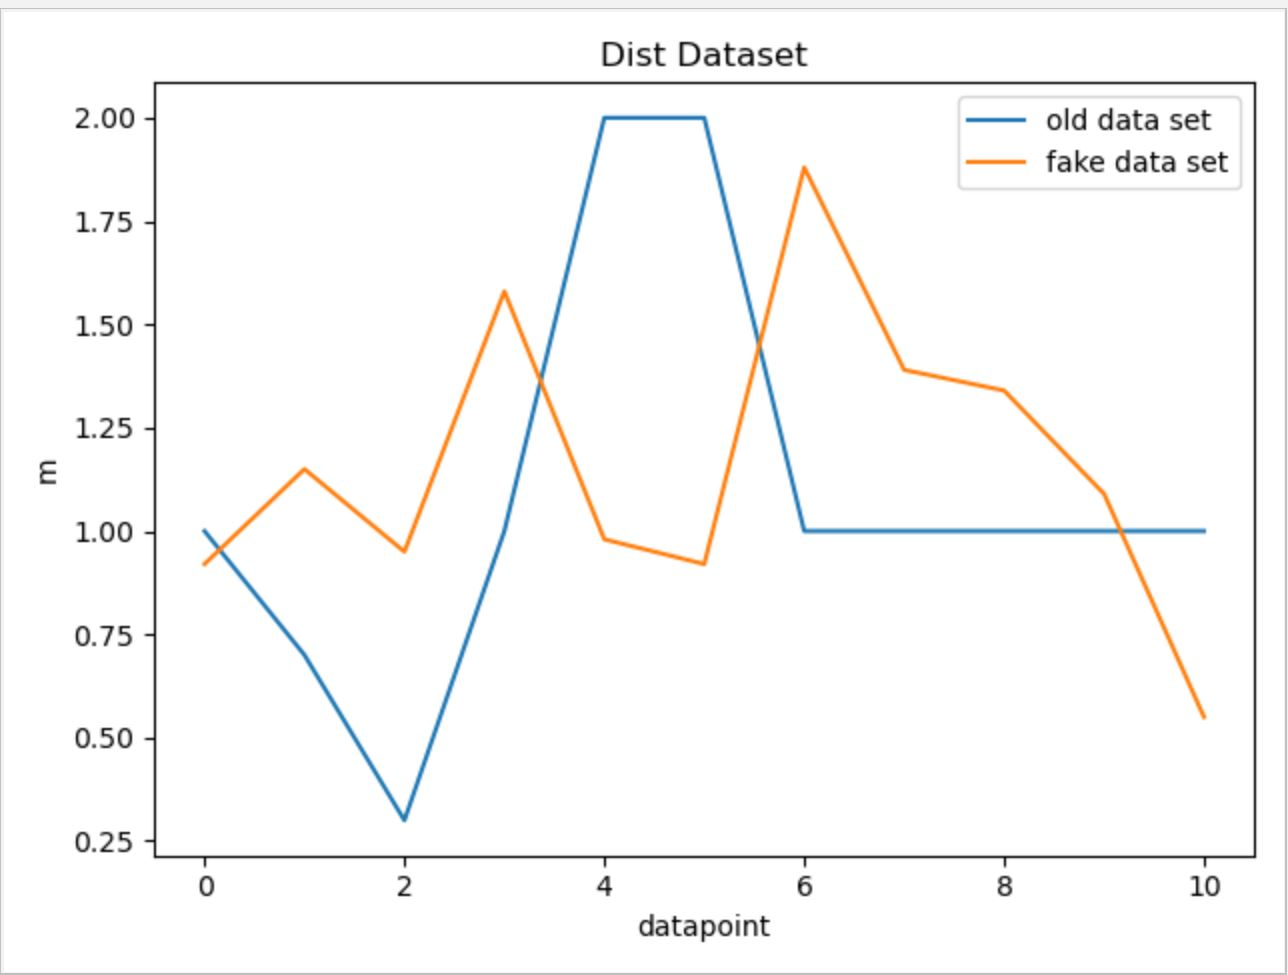
\includegraphics[width=0.50000\textwidth]{./images/Elev Data.JPG} For
Heart data:\\
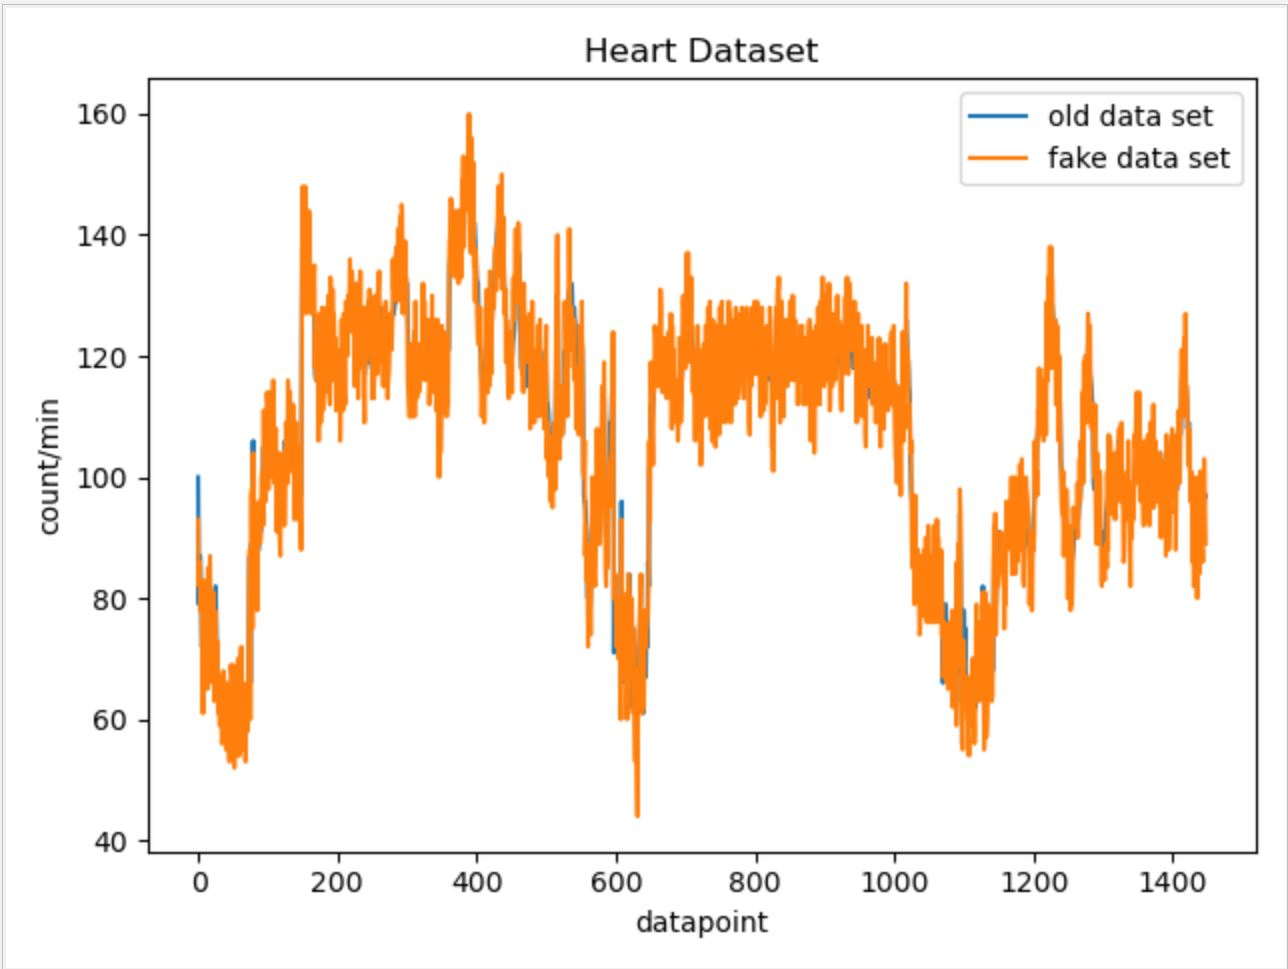
\includegraphics[width=0.50000\textwidth]{./images/Heart Data.JPG} For
Steps data:\\
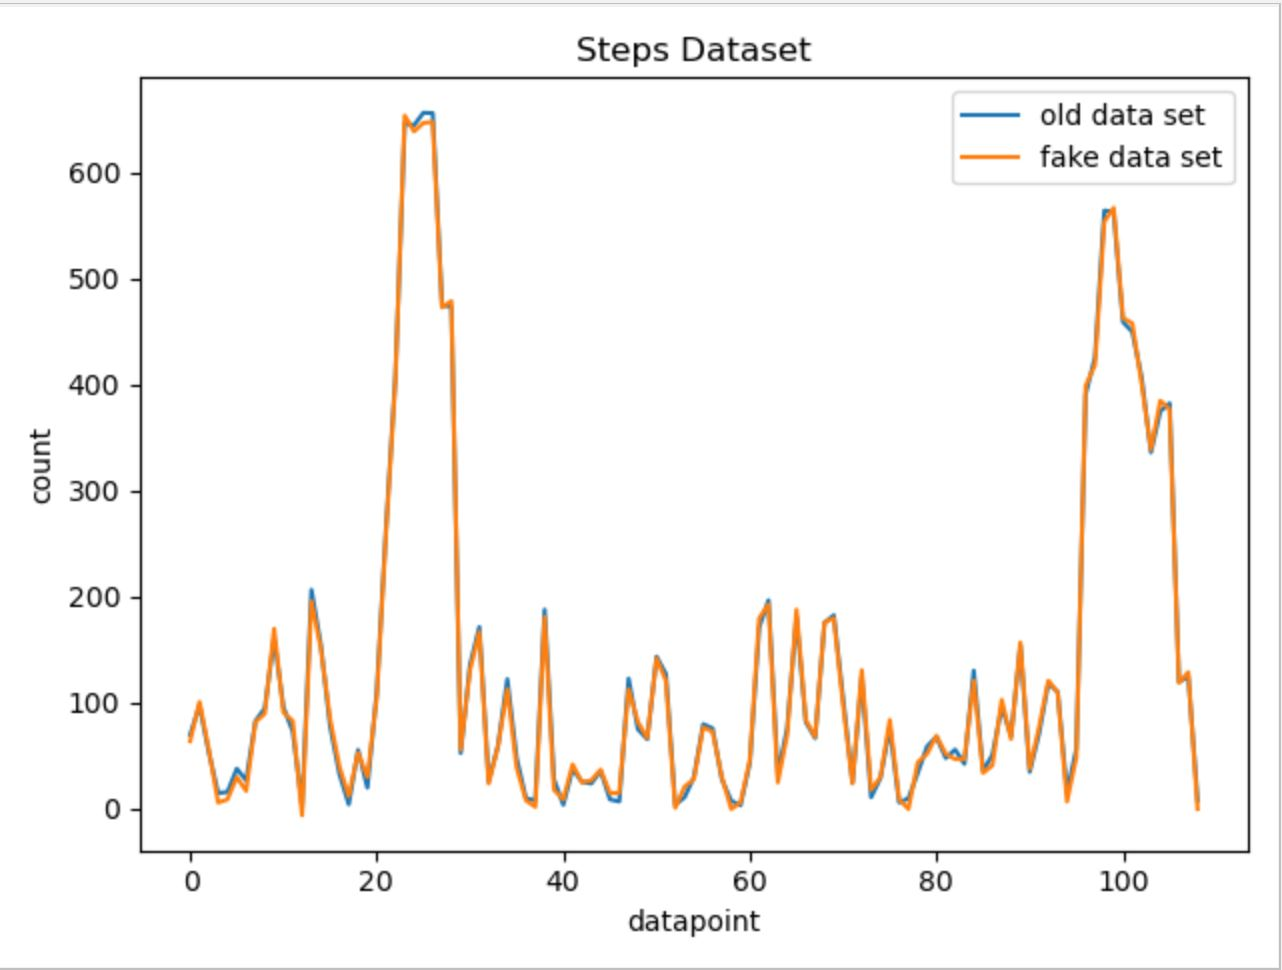
\includegraphics[width=0.50000\textwidth]{./images/Steps Data.JPG}

\subsection{How to run the scripts?}\label{how-to-run-the-scripts}

In order to run the scripts, some modifications to the
GenerateFakeData.py are needed. There are three parameters that need
modification: folder\_name\_list, real\_name\_list, and path.
``folder\_name\_list'' tells the name of the folders that will contain
the dummy data. ``real\_name\_list'' tells the name of the reference
files being used to generate dummy data. ``path'' is the current
directory. Once these three parameters are set up correctly, just
directly run the GenerateFakeData.py script with no input.

\subsection{Potential improvements}\label{potential-improvements}

Because our dummy data generation script is specifically modified for
each data set, if in the future a new type of data appears, we need to
rewrite our code in order to accommodate the new data type. Therefore,
we can improve our code by applying more statictical knowledge so that
the code can be applied to generate dummy data from more different data
types.

\section{Creating a connection between API
Endpoints}\label{creating-a-connection-between-api-endpoints}

\subsection{List of API end-points:}\label{list-of-api-end-points}

\begin{enumerate}
\def\labelenumi{\arabic{enumi}.}
\tightlist
\item
  Front-End Patient User input to the database
\item
  Biometric Data from the FitBit API to the database
\item
  Data from the database to the RShiny Dashboard for visualization
\end{enumerate}

\subsection{What framework we are going to
use?}\label{what-framework-we-are-going-to-use}

We are currently looking to use the framework Express.js to write the
routes between the database and various API endpoints.

Express is a fast, light-weight web framework for Node.js. Express is a
pretty good framework. It's the most popular node application framework
out there. Express is widely used as middleware in node apps as it helps
to organize your app into a MVC architecture. It's the E of the popular
MEAN stack. Express manages following things very easily:

\begin{itemize}
\tightlist
\item
  Routing
\item
  Sessions
\item
  HTTP requests
\item
  Error handling
\end{itemize}

At times writing code from scratch for above things can be time
consuming. But by using express it's only a matter of few methods.
Express also helps in organizing your code.

\href{https://medium.com/@onejohi/building-a-simple-rest-api-with-nodejs-and-express-da6273ed7ca9}{Link
to set up Node}

\subsection{Setting up SQL database
connection:}\label{setting-up-sql-database-connection}

We created a connection with the MariaDB database in our Node Rest API
server to be able to send and receive data. The following link shows a
tutorial on how we set up the connection.

\href{https://bezkoder.com/node-js-rest-api-express-mysql/}{Link to
setup SQL connection in Node}

\subsection{Design of the Routes}\label{design-of-the-routes}

There are five kinds of routes:

\textbf{GET}: The GET method requests a representation of the specified
resource. Requests using GET should only retrieve data and should have
no other effect.

\textbf{POST}: The POST method requests that the server accept the
entity enclosed in the request as a new subordinate of the web resource
identified by the URI. The data POSTed might be, for example, an
annotation for existing resources; a message for a bulletin board,
newsgroup, mailing list, or comment thread; a block of data that is the
result of submitting a web form to a data-handling process; or an item
to add to a database.

\textbf{PUT}: The PUT method requests that the enclosed entity be stored
under the supplied URI. If the URI refers to an already existing
resource, it is modified; if the URI does not point to an existing
resource, then the server can create the resource with that URI.

\textbf{DELETE}: The DELETE method deletes the specified resource.

\textbf{PATCH}: The PATCH method applies partial modifications to a
resource

\section{Hosting the database on a
Server}\label{hosting-the-database-on-a-server}

\subsection{Issues faced with hosting a database on
Scholar:}\label{issues-faced-with-hosting-a-database-on-scholar}

\begin{enumerate}
\def\labelenumi{\arabic{enumi}.}
\tightlist
\item
  Scholar is a small computer cluster, suitable for classroom learning
  about high performance computing (HPC).
\item
  It can be accessed as a typical cluster, with a job scheduler
  distributing batch jobs onto its worker nodes, or as an interactive
  resource, with software packages available through a desktop-like
  environment on its login servers.
\item
  We tried to create a connection to the sql server hosted on this
  server from our local but we faced issues because there was a firewall
  preventing access to the database from a foreign server
\item
  We tried running our Backend API on scholar but we were unable to
  install NodeJS, MySQLWorkbench and other packages on the server
  without authorization.
\end{enumerate}

\subsection{Work around}\label{work-around}

\begin{enumerate}
\def\labelenumi{\arabic{enumi}.}
\item
  In order to install packages on scholar, we are expected to make
  requests to the administration with a list of all program lines to run
  in the form of a SLURM job.
\item
  The Simple Linux Utility for Resource Management (SLURM) is a system
  providing job scheduling and job management on compute clusters. With
  SLURM, a user requests resources and submits a job to a queue. The
  system will then take jobs from queues, allocate the necessary nodes,
  and execute them.
\item
  To submit work to a SLURM queue, you must first create a job
  submission file.
\end{enumerate}

More info can be found at the following link:
\href{https://www.rcac.purdue.edu/knowledge/weber/run/slurm}{SLURM Job}

\subsection{How we proceeded}\label{how-we-proceeded}

Since we have to make a request each time we have to install a package,
we decided to make just one request with a complete list of all
installation. As a result, we wanted to host a temporary database on AWS
that we can connect to and test on using our local machine.

We created a copy of the entire database on AWS with the following
credentials:

\begin{itemize}
\tightlist
\item
  Hostname: rnr56s6e2uk326pj.cbetxkdyhwsb.us-east-1.rds.amazonaws.com
\item
  Username: cb3i17t0aqn6a4ff
\item
  Password: e2l4k9zn24shcj42
\end{itemize}

\section{Adding data to the database}\label{adding-data-to-the-database}

\subsection{Adding a CSV to the
database}\label{adding-a-csv-to-the-database}

\begin{enumerate}
\def\labelenumi{\arabic{enumi}.}
\tightlist
\item
  The data engineering team had made a script that creates a CSV file
  with all the users FitBit data when they make a request to the API
\item
  We decided to make a python script to load this csv data onto the
  database we hosted on AWS.
\end{enumerate}

\subsection{POST information}\label{post-information}

\begin{enumerate}
\def\labelenumi{\arabic{enumi}.}
\item
  The JSON to add a datapoint to the database is as follows:

\begin{verbatim}
 obj = {'collection_date': row["Date"],
       'steps': row["Steps"],
       'floors_climbed': row["Floors Climbed"],
       'total_miles': row["Total Miles"],
       'lightly_active_miles': ["Lightly Active Miles"],
       'moderately_active_miles': row["Moderately Active Miles"],
       'very_active_miles': row["Very Active Miles"],
       'sedentary_minutes': row["Sedentary Minutes"],
       'lightly_active_minutes': row["Lightly Active Minutes"],
       'fairly_active_minutes': row["Fairly Active Minutes"],
       'very_active_minutes': row["Very Active Minutes"],
       'hr30_100_minutes': row["HR 30-100 Minutes"],
       'hr100_140_minutes': row["HR 100-140 Minutes"],
       'hr140_170_minutes': row["HR 140-170 Minutes"],
       'hr170_220_minutes': row["HR 170-220 Minutes"],
       'average_resting_heartrate': row["Average Resting HR"],
       'bmi': row["BMI"],
       'sleep_efficiency': row["Sleep Efficiency"],
       'weight': row["Weight"],
       'minutes_asleep': row["Minutes Alseep"],
       'fbusername': row["username"]
       }
\end{verbatim}
\item
  We made structures in this form by reading the CSV information into a
  pandas dataframe and made a post request to our API
\end{enumerate}

\subsection{Patient information and Study Specific
Data}\label{patient-information-and-study-specific-data}

The patient information is sent to the database form a webpage which
will be used by Merck Scientists to load the patients they are studying
during a clinical trial.

The JSON for a patient is as follows:

\begin{verbatim}
{
  patient_id,
  fbusername,
  first_name,
  last_name,
  gender,
  date_of_birth,
  height
}
\end{verbatim}

The JSON for the study data is as follows:

\begin{verbatim}
{
    patient_id,
    input_date,
    family_history_cancer,
    family_history_heart_disease,
    diagnostic_notes
}
\end{verbatim}

\section{Firebase and Login System for the Phone
App}\label{firebase-and-login-system-for-the-phone-app}

(This part is also in frontend team's documentation, because it is
relavant to both of the teams) Because our app's users are patients and
their information is very confidential, It is important to implement our
login and authentication system securely. Instead of building a secure
login system from scratch by ourselves, we chose to use a pre-existing
login authentication solution--firebase. In firebase, users' passwords
are first encrypted and then stored. Even if hackers successfully gain
access to firebase's database, they still would not know the passwords
because everything stored there is the encrypted version.

The next step is to incorporate the firebase login system into our own
database. Our current thought is that, once the user logs in through
firebase, they will receive a key from firebase. Then whenever they want
to modify or store data in our database, they send the key along with
every HTTP request. The backend would check the correctness of the key
and only allow accessibility if the key is correct.

\chapter{Front End Team}\label{front-end-team}

\section{Utilization of Third Party
Software}\label{utilization-of-third-party-software}

The sole third party software being used in our application is Firebase,
a Google based software designed for user authentication purposes. The
codes upon which this app is built are independently developed by our
team members. The data used to develop the app is Biometric data
collected currently only through Fitbit, though the goal is to expand
the collection capability to be able to obtain Apple Watch data as well.
This data is accessed through an external Merck API which is linked
through an SCTP request.

\section{Software Components}\label{software-components}

Our application has five main sections. The first section covers
everything prior to successful user login. This includes the login page
along with Firebase authentication. The second section is the home page
where users would be able to view displayed data pertaining to
themselves. The third section is a graphics page where graphs are
presented, informing users their health progress and their default
Fitbit data. The fourth section is the question response page where
users are guided to complete questionnaires for the purpose of data
collection beyond the default data collected by the wearable device. The
final section is the user setting page where users can view and edit
their information and settings; a log out option is also available
through this section.

\subsection{Pre-Login section}\label{pre-login-section}

The pre-login section has been mostly completed, however we are yet to
integrate the firebase completely within the page itself. The firebase
portion of this page has been created. This portion does not contain any
important functions besides the absolute base, standard functions
required by firebase to run. The login page aspect of this section has a
few important functions. For one, the entire app is stacked into a
function called Loginpage to make it harder for consumers to access. The
page runs similar to as expected. There's a space to enter a username
and password and a login button which gives a notification that you are
being logged in. TextInput and TouchableOpacity were both enabled to
allow popup notifications and username and password entry. For the
password entry, secureTextEntry was set to true, which turns the letters
into dots as they are typed.

\subsection{Home Page Section}\label{home-page-section}

The home page section is very simple; the current home page is where
basic data such as sleep, heart rate, etc would be presented in a clean
fashion as a summary. It is our goal to implement additional features to
this page along with an in depth description of user's data through the
graphics page.

\subsection{Question Response Section}\label{question-response-section}

The question response page collects data to further bolster the health
data collected by the users' wearables. It has many implemented
functionality to facilitate the data collection process, for example, it
displays information based on users' previous responses; This is done
using the constructor function. It also uses the onChangeText function
for the sake of clarity when the user selects a value. Ideally, a camera
feature will be made available on this page in the event that a user
wishes to upload an image to further elaborate on their health
conditions.

\subsection{User Setting Section}\label{user-setting-section}

Finally, There is the user information page which contains all of the
basic testing information and personal information that clinical trial
patient would preferably want to know, users can also log out through
this page if they so wishes. Ideally, this page would also bare a camera
feature which allow users to set a profile picture. Codes are stored in
a function creatively named Code, and consists of basic text and image
functions with one TouchableOpacity function so far to log the user out.

\end{document}
